        %%******************************************%%
        %%                                          %%
        %%        Modello di tesi di laurea         %%
        %%            di Andrea Giraldin            %%
        %%                                          %%
        %%             2 novembre 2012              %%
        %%                                          %%
        %%******************************************%%


% I seguenti commenti speciali impostano:
% 1. 
% 2. PDFLaTeX come motore di composizione;
% 3. tesi.tex come documento principale;
% 4. il controllo ortografico italiano per l'editor.

% !TEX encoding = UTF-8
% !TEX TS-program = pdflatex
% !TEX root = tesi.tex
% !TEX spellcheck = it-IT

\documentclass[10pt,                    % corpo del font principale
               a4paper,                 % carta A4
               twoside,                 % impagina per fronte-retro
               openright,               % inizio capitoli a destra
               english,                 
               italian,                 
               ]{book}    

%**************************************************************
% Importazione package
%************************************************************** 

%\usepackage{amsmath,amssymb,amsthm}    % matematica

\usepackage[T1]{fontenc}                % codifica dei font:
                                        % NOTA BENE! richiede una distribuzione *completa* di LaTeX

\usepackage[utf8]{inputenc}             % codifica di input; anche [latin1] va bene
                                        % NOTA BENE! va accordata con le preferenze dell'editor

\usepackage[english, italian]{babel}    % per scrivere in italiano e in inglese;
                                        % l'ultima lingua (l'italiano) risulta predefinita

\usepackage{bookmark}                   % segnalibri

\usepackage{caption}                    % didascalie

\usepackage{chngpage,calc}              % centra il frontespizio

\usepackage{csquotes}                   % gestisce automaticamente i caratteri (")

\usepackage{emptypage}                  % pagine vuote senza testatina e piede di pagina

\usepackage{epigraph}			% per epigrafi

\usepackage{eurosym}                    % simbolo dell'euro

%\usepackage{indentfirst}               % rientra il primo paragrafo di ogni sezione

\usepackage{graphicx}                   % immagini

\usepackage{hyperref}                   % collegamenti ipertestuali

\usepackage[binding=5mm]{layaureo}      % margini ottimizzati per l'A4; rilegatura di 5 mm

\usepackage{listings}                   % codici

\usepackage{microtype}                  % microtipografia

\usepackage{mparhack,fixltx2e,relsize}  % finezze tipografiche

\usepackage{nameref}                    % visualizza nome dei riferimenti                                      

\usepackage[font=small]{quoting}        % citazioni

\usepackage{subfig}                     % sottofigure, sottotabelle

\usepackage[italian]{varioref}          % riferimenti completi della pagina

%\usepackage[dvipsnames]{xcolor}         % colori

\usepackage{booktabs}                   % tabelle                                       
\usepackage{tabularx}                   % tabelle di larghezza prefissata                                    
\usepackage{longtable}                  % tabelle su più pagine                                        
\usepackage{ltxtable}                   % tabelle su più pagine e adattabili in larghezza

\usepackage{lmodern}
\usepackage[table]{xcolor}
\usepackage{array}
\usepackage{colortbl}
\usepackage{verbatim}


\usepackage[toc, acronym]{glossaries}   % glossario
                                        % per includerlo nel documento bisogna:
                                        % 1. compilare una prima volta tesi.tex;
                                        % 2. eseguire: makeindex -s tesi.ist -t tesi.glg -o tesi.gls tesi.glo
                                        % 3. eseguire: makeindex -s tesi.ist -t tesi.alg -o tesi.acr tesi.acn
                                        % 4. compilare due volte tesi.tex.

\usepackage[backend=biber,style=verbose-ibid,hyperref,backref]{biblatex}
                                        % eccellente pacchetto per la bibliografia; 
                                        % produce uno stile di citazione autore-anno; 
                                        % lo stile "numeric-comp" produce riferimenti numerici
                                        % per includerlo nel documento bisogna:
                                        % 1. compilare una prima volta tesi.tex;
                                        % 2. eseguire: biber tesi
                                        % 3. compilare ancora tesi.tex.


%**************************************************************
% file contenente le impostazioni della tesi
%**************************************************************

%**************************************************************
% Frontespizio
%**************************************************************

% Autore
\newcommand{\myName}{Federico Perin}                                    
\newcommand{\myTitle}{Analisi, progettazione e sviluppo di un motore conversazionale per una piattaforma di gestione della forza lavoro}

% Tipo di tesi                   
\newcommand{\myDegree}{Tesi di laurea triennale}

% Università             
\newcommand{\myUni}{Università degli Studi di Padova}

% Facoltà       
\newcommand{\myFaculty}{Corso di Laurea in Informatica}

% Dipartimento
\newcommand{\myDepartment}{Dipartimento di Matematica "Tullio Levi-Civita"}

% Titolo del relatore
\newcommand{\profTitle}{Prof.}

% Relatore
\newcommand{\myProf}{Claudio Enrico Palazzi}

% Luogo
\newcommand{\myLocation}{Padova}

% Anno accademico
\newcommand{\myAA}{2019-2020}

% Data discussione
\newcommand{\myTime}{Settembre 2020}

\newcommand{\paginavuota}{\newpage\null\thispagestyle{empty}}

%**************************************************************
% Impostazioni di impaginazione
% see: http://wwwcdf.pd.infn.it/AppuntiLinux/a2547.htm
%**************************************************************

\setlength{\parindent}{14pt}   % larghezza rientro della prima riga
\setlength{\parskip}{0pt}   % distanza tra i paragrafi


%**************************************************************
% Impostazioni di biblatex
%**************************************************************
\bibliography{bibliografia} % database di biblatex 

\defbibheading{bibliography} {
    \cleardoublepage
    \phantomsection 
    \addcontentsline{toc}{chapter}{\bibname}
    \chapter*{\bibname\markboth{\bibname}{\bibname}}
}

\setlength\bibitemsep{1.5\itemsep} % spazio tra entry

\DeclareBibliographyCategory{opere}
\DeclareBibliographyCategory{web}

\addtocategory{opere}{womak:lean-thinking}
\addtocategory{web}{site:agile-manifesto}

\defbibheading{opere}{\section*{Riferimenti bibliografici}}
\defbibheading{web}{\section*{Siti Web consultati}}


%**************************************************************
% Impostazioni di caption
%**************************************************************
\captionsetup{
    tableposition=top,
    figureposition=bottom,
    font=small,
    format=hang,
    labelfont=bf
}

%**************************************************************
% Impostazioni di glossaries
%**************************************************************

%**************************************************************
% Acronimi
%**************************************************************
\renewcommand{\acronymname}{Acronimi e abbreviazioni}

\newacronym[description={\glslink{apig}{Application Program Interface}}]
    {api}{API}{Application Program Interface}
    
\newacronym[description={\glslink{AWMSg}{Advanced Workforce Management System}}]
{AWMS}{AWMS}{Advanced Workforce Management System}

\newacronym[description={\glslink{umlg}{Unified Modeling Language}}]
    {uml}{UML}{Unified Modeling Language}
\newacronym[description={Test End to End}]
{test e2e}{E2E}{test End to End}
\newacronym[description={Internazionalizzazione}]
{i18n}{i18n}{internazionalizzazione}

%**************************************************************
% Glossario
%**************************************************************
\renewcommand{\glossaryname}{Glossario}

\newglossaryentry{apig}
{
    name=\glslink{api}{API},
    text=Application Program Interface,
    sort=api,
    description={In informatica con il termine \emph{Application Programming Interface API} (ing. interfaccia di programmazione di un'applicazione) si indica ogni insieme di procedure disponibili al programmatore, di solito raggruppate a formare un set di strumenti specifici per l'espletamento di un determinato compito all'interno di un certo programma. La finalità è ottenere un'astrazione, di solito tra l'hardware e il programmatore o tra software a basso e quello ad alto livello semplificando così il lavoro di programmazione}
}

\newglossaryentry{umlg}
{
    name=\glslink{uml}{UML},
    text=UML,
    sort=uml,
    description={in ingegneria del software \emph{UML, Unified Modeling Language} (ing. linguaggio di modellazione unificato) è un linguaggio di modellazione e specifica basato sul paradigma object-oriented. L'\emph{UML} svolge un'importantissima funzione di ``lingua franca'' nella comunità della progettazione e programmazione a oggetti. Gran parte della letteratura di settore usa tale linguaggio per descrivere soluzioni analitiche e progettuali in modo sintetico e comprensibile a un vasto pubblico}
}

\newglossaryentry{AWMSg}
{
	name=\glslink{AWMS}{AWMS},
	text=Advanced Workforce Management System,
	sort=AWMS,
	description={È una soluzione software che utilizza algoritmi di \gls{machine learning}, per risolvere uno dei problemi cardine di un \gls{plant manager} ovvero, la pianificazione ottimale della forza lavoro che ha disposizione. L'obbiettivo principale della soluzione è quello di pianificare la persona giusta al posto giusto in base alle competenze tecniche possedute del lavoratore}
}

\newglossaryentry{Electrolux}
{
	name={Electrolux},
	text=Electrolux,
	sort=electrolux,
	description={Electrolux è una multinazionale svedese produttrice di elettrodomestici con sede a Stoccolma}
}

\newglossaryentry{machine learning}
{
	name={Machine learning},
	text=Machine learning,
	sort=machine learning,
	description={Nell'ambito dell'informatica, l'apprendimento automatico è una variante alla programmazione tradizionale nella quale in una macchina si predispone l'abilità di apprendere qualcosa dai dati in maniera autonoma, senza istruzioni esplicite}
}

\newglossaryentry{plant manager}
{
	name={Plant manager},
	text=Plant manager,
	sort=plant manager,
	description={Detto anche responsabile di stabilimento, è colui che presiede e organizza le operazioni quotidiane degli impianti di produzione aziendali, di cui deve assicurare il funzionamento ottimale ed efficiente. Si occupa dei lavoratori, assegnando funzioni e ruoli, definendo orari di lavoro e produzione, formando i neo assunti. Raccoglie e analizza i dati di produzione per trovare eventuali spazi di miglioramento. Si occupa della sicurezza dei lavoratori e quella degli impianti; monitora le apparecchiature di produzione e, in caso di necessità, della loro riparazione o sostituzione}
}

\newglossaryentry{bot}
{
	name={Bot},
	text=bot,
	sort=bot,
	description={È un software progettato per simulare una conversazione con un essere umano. Lo scopo principale di questi software è quello di simulare un comportamento umano e sono a volte definiti anche agenti intelligenti e vengono usati per vari scopi come la guida in linea, per rispondere alle FAQ degli utenti che accedono a un sito. In alcuni utilizzano sofisticati sistemi di elaborazione del linguaggio naturale, ma molti si limitano a eseguire la scansione delle parole chiave nella finestra di input e fornire una risposta con le parole chiave più corrispondenti}
}

\newglossaryentry{QR code}
{
	name={QR code},
	text=QR code,
	sort=qr-code,
	description={È un codice a barre bidimensionale (o codice 2D), ossia a matrice, composto da moduli neri disposti all'interno di uno schema bianco di forma quadrata, impiegato tipicamente per memorizzare informazioni generalmente destinate a essere lette tramite uno smartphone}
}

\newglossaryentry{WebSocket}
{
	name={WebSocket},
	text=WebSocket,
	sort=websocket,
	description={È una tecnologia web che fornisce canali di comunicazione a due direzioni cioè gli interlecutori possono sia inviare sia ricevere contemporaneamente attraverso una singola connessione TCP}
}

\newglossaryentry{SCRUM}
{
	name={SCRUM},
	text=SCRUM,
	sort=scrum,
	description={È un framework agile per la gestione del ciclo di sviluppo del software, iterativo ed incrementale, concepito per gestire progetti e prodotti software o applicazioni di sviluppo. Nel proprio manifesto prevede i seguenti punti che lo caratterizzano, le persone e le interazioni sono più importanti dei processi e dei strumenti, meglio avere da subito software funzionante che documentazione ampia, meglio una collaborazione con il cliente piuttosto che fare una negoziazione del contratto, essere in grando di rispondere ai cambiamenti piuttosto che rispettare un piano. 
	I progetti Scrum progrediscono attraverso una serie di sprint che hanno una durata massima di un mese. Negli sprint vengono decisi quali requisiti devono essere soddisfatti, e quindi successivamente, progettati, implementati e testati}
}
\newglossaryentry{framework}{
	name={Framework},
	text=framework,
	sort=framework,
	description={In informatica con il termine framework 
	si indica un insieme di elementi software che un programmatore può usare o modificare per realizzare un programma. Rappresenta un astrazione composta da elementi universali e riutilizzabili con lo scopo di facilitare lo sviluppo di un programma e di far applicare buone norme di programmazione. Inoltre, un framework può offrire programmi di supporto, librerie, compilatori e documentazione per l'utilizzo}
}
\newglossaryentry{iOS}{
	name={iOS},
	text=iOS,
	sort=iOS,
	description={È un sistema operativo \emph{mobile} sviluppato da Apple per iPhone, iPod touch e iPad. Le versioni principali di iOS vengono distribuite ogni anno. L'attuale versione, iOS 13, è stata distribuita al pubblico il 19 settembre 2019}
}
\newglossaryentry{Android}{
	name={Android},
	text=Android,
	sort=Android,
	description={È un sistema operativo per dispositivi \emph{mobile} sviluppato da Google e basato sul kernel Linux, progettato principalmente per \emph{smartphone} e \emph{tablet}, interfacce utente specializzate per televisori (Android TV), automobili (Android Auto), orologi da polso (Wear OS), occhiali (Google Glass). L'attuale versione è Android 11}
}
\newglossaryentry{architettura}{
	name={Architettura},
	text=Android,
	sort=Android,
	description={In informatica con il termine architettura, in questo caso intesa come architettura software, l'organizzazione fondamentale di un sistema, definita dai suoi componenti, dalle relazioni reciproche tra i componenti e con l'ambiente, e i principi che ne governano la progettazione e l'evoluzione}
}
\newglossaryentry{linguaggio di markup}{
	name={Linguaggio di markup},
	text=linguaggio di markup,
	sort=linguaggio di markup,
	description={In informatica con il termine linguaggio di markup, un gruppo di regole detti marcatori, attraverso le quali vengono descritti i meccanismi di rappresentazione di un testo}
}
\newglossaryentry{browser web}{
	name={Browser web},
	text=browser web,
	sort=browser web,
	description={In informatica si intende un'applicazione per l'acquisizione, la presentazione e la navigazione di risorse sul web. Permette la visualizzazione dei contenuti ipertestuali, e la riproduzione di contenuti multimediali. Tra i browser più popolari vi sono Google Chrome, Internet Explorer, Mozilla Firefox, Microsoft Edge, Safari, Opera}
}

\newglossaryentry{applicazione nativa}{
	name={Applicazione nativa},
	text=applicazione nativa,
	sort=applicazione nativa,
	description={In informatica si intende un'applicazione scritta e compilata per una specifica piattaforma utilizzando i linguaggi di programmazione e librerie supportati dal particolare sistema operativo \emph{mobile}}
}

\newglossaryentry{applicazione web mobile}{
	name={Applicazione web mobile},
	text=applicazione web mobile,
	sort=applicazione web mobile,
	description={In informatica si intende pagine web ottimizzate per dispositivi \emph{mobile} scritte utilizzando tecnologie web, in particolare HTML, JavaScript e CSS. Inoltre, le applicazioni web non possono accedere alle funzionalità del dispositivo ad'esempio la fotocamera}
}

\newglossaryentry{applicazione ibrida}{ %va a benzina ma anche con l'elettricità
	name={Applicazione ibrida},
	text=applicazione ibrida,
	sort=applicazione ibrida,
	description={In informatica si intende applicazioni sviluppate con tecnologie web e vengono eseguite localmente all’interno di un’applicazione nativa. Grazie a cio possono interagire con il dispositivo ad'esempio utilizzare la fotocamera}
}

\newglossaryentry{notifica push}{ 
	name={Notifica push},
	text=notifica push,
	sort=notifica pusha,
	description={In informatica si intende un tipo di messaggistica istantanea grazie alla quale il messaggio perviene al destinatario senza che questo debba effettuare un'operazione di scaricamento. Tale modalità è quella tipicamente usata da applicazioni come \emph{WhatsApp} o da servizi di sistemi operativi come \gls{Android}\ap{[g]}, oppure da numerose applicazioni derivate da siti web come, ad esempio, il servizio meteo o quello delle notizie}
}

\newglossaryentry{licenza MIT}{ 
	name={Licenza MIT},
	text=licenza MIT,
	sort=licenza MIT,
	description={La Licenza MIT è una licenza di software libero. È una licenza permissiva, cioè permette il riutilizzo nel software proprietario sotto la condizione che la licenza sia distribuita con tale software}
}

\newglossaryentry{JSON}{ 
	name=\glslink{JSON}{JSON},
	text=JSON,
	sort=JSON,
	description={ È un semplice formato adatto all'interscambio di dati fra applicazioni client/server. Risulta essere facile da comprendere e da scrivere per le persone mentre per le macchine risulta essere un formato leggero e veloce da analizzare}
}

\begin{comment}
\newglossaryentry{e2eg}
{
	name=\glslink{test e2e}{E2E},
	text=Test End to End,
	sort=test End to End,
	description={Con il termine test end-to-end (end-to-end testing) si intende quell’attività di testing dell’interfaccia grafica vista dagli utenti del programma dall’inizio fino alla fine. In altre parole rappresenta una metodologia utilizzata per verificare se il flusso di un’applicazione si sta comportando come progettato dall’inizio fino alla fine senza che vengano rilevati dei errori che andrebbero a inficiare sulla qualità dell’applicazione stessa}
}

Parole da aggiungere

http
pooling
client
server
Client/Server
SDK -> acronimo HTML e CSS http
open-source
JSON
API REST
\end{comment}
 % database di termini
\makeglossaries


%**************************************************************
% Impostazioni di graphicx
%**************************************************************
\graphicspath{{immagini/}} % cartella dove sono riposte le immagini


%**************************************************************
% Impostazioni di hyperref
%**************************************************************
\hypersetup{
    %hyperfootnotes=false,
    %pdfpagelabels,
    %draft,	% = elimina tutti i link (utile per stampe in bianco e nero)
    %colorlinks=true,
    %linktocpage=true,
    pdfstartpage=1,
    pdfstartview=FitV,
    % decommenta la riga seguente per avere link in nero (per esempio per la stampa in bianco e nero)
    colorlinks=false, linktocpage=false, pdfborder={0 0 0}, pdfstartpage=1, pdfstartview=FitV,
    breaklinks=true,
    pdfpagemode=UseNone,
    pageanchor=true,
    pdfpagemode=UseOutlines,
    plainpages=false,
    bookmarksnumbered,
    bookmarksopen=true,
    bookmarksopenlevel=1,
    hypertexnames=true,
    pdfhighlight=/O,
    %nesting=true,
    %frenchlinks,
    urlcolor=webbrown,
    linkcolor=RoyalBlue,
    citecolor=webgreen,
    %pagecolor=RoyalBlue,
    %urlcolor=Black, linkcolor=Black, citecolor=Black, %pagecolor=Black,
    pdftitle={\myTitle},
    pdfauthor={\textcopyright\ \myName, \myUni, \myFaculty},
    pdfsubject={},
    pdfkeywords={},
    pdfcreator={pdfLaTeX},
    pdfproducer={LaTeX}
}

%**************************************************************
% Impostazioni di itemize
%**************************************************************
\renewcommand{\labelitemi}{$\ast$}

%\renewcommand{\labelitemi}{$\bullet$}
%\renewcommand{\labelitemii}{$\cdot$}
%\renewcommand{\labelitemiii}{$\diamond$}
%\renewcommand{\labelitemiv}{$\ast$}


%**************************************************************
% Impostazioni di listings
%**************************************************************
\lstset{
    language=[LaTeX]Tex,%C++,
    keywordstyle=\color{RoyalBlue}, %\bfseries,
    basicstyle=\small\ttfamily,
    %identifierstyle=\color{NavyBlue},
    commentstyle=\color{Green}\ttfamily,
    stringstyle=\rmfamily,
    numbers=none, %left,%
    numberstyle=\scriptsize, %\tiny
    stepnumber=5,
    numbersep=8pt,
    showstringspaces=false,
    breaklines=true,
    frameround=ftff,
    frame=single
} 


%**************************************************************
% Impostazioni di xcolor
%**************************************************************
\definecolor{webgreen}{rgb}{0,.5,0}
\definecolor{webbrown}{rgb}{.6,0,0}
\definecolor{SchoolColor}{rgb}{0.71, 0, 0.106}
%%Colori per le tabelle
\definecolor{grigetto}{RGB}{234, 234, 234}
\definecolor{rossoep}{RGB}{164,60,59}
\definecolor{darkblue}{RGB}{59,77,95}
\definecolor{giallo}{RGB}{251,168,11}
\definecolor{verde}{RGB}{87,180,0}
\definecolor{grigio}{gray}{.7}
\definecolor{grigioChiaro}{gray}{.9}

\newcommand{\classdesc}[2]{\item[\textbf{#1:}] #2}
\newcommand{\intest}[1]{\multicolumn{1}{>{\columncolor{rossoep}}c}{\textbf{#1}}}
\newcolumntype{Z}{>{\centering\arraybackslash}X}
\renewcommand{\tabularxcolumn}[1]{>{\arraybackslash}m{#1}}


%**************************************************************
% Altro
%**************************************************************

\newcommand{\omissis}{[\dots\negthinspace]} % produce [...]

% eccezioni all'algoritmo di sillabazione
\hyphenation
{
    ma-cro-istru-zio-ne
    gi-ral-din
}

\newcommand{\sectionname}{sezione}
\addto\captionsitalian{\renewcommand{\figurename}{Figura}
                       \renewcommand{\tablename}{Tabella}}

\newcommand{\glsfirstoccur}{\ap{{[g]}}}

\newcommand{\intro}[1]{\emph{\textsf{#1}}}

%**************************************************************
% Environment per ``rischi''
%**************************************************************
\newcounter{riskcounter}                % define a counter
\setcounter{riskcounter}{0}             % set the counter to some initial value

%%%% Parameters
% #1: Title
\newenvironment{risk}[1]{
    \refstepcounter{riskcounter}        % increment counter
    \par \noindent                      % start new paragraph
    \textbf{\arabic{riskcounter} #1}   % display the title before the 
                                        % content of the environment is displayed 
}{
    \par\medskip
}

\newcommand{\riskname}{Rischio}

\newcommand{\riskdescription}[1]{\textbf{\\Descrizione:} #1}

\newcommand{\risksolution}[1]{\textbf{\\Soluzione:} #1}

%**************************************************************
% Environment per ``use case''
%**************************************************************
\newcounter{usecasecounter}             % define a counter
\setcounter{usecasecounter}{0}          % set the counter to some initial value

%%%% Parameters
% #1: ID
% #2: Nome
\newenvironment{usecase}[2]{
    \renewcommand{\theusecasecounter}{\usecasename #1}  % this is where the display of 
                                                        % the counter is overwritten/modified
    \refstepcounter{usecasecounter}             % increment counter
    \vspace{10pt}
    \par \noindent                              % start new paragraph
    {\large \textbf{\usecasename #1: #2}}       % display the title before the 
                                                % content of the environment is displayed 
    \medskip
}{
    \medskip
}

\newcommand{\usecasename}{UC}

\newcommand{\usecaseactors}[1]{\textbf{\\Attori Principali:} #1. \vspace{4pt}}
\newcommand{\usecasepre}[1]{\textbf{\\Precondizioni:} #1. \vspace{4pt}}
\newcommand{\usecasedesc}[1]{\textbf{\\Scenario Principale:} #1 \vspace{4pt}}
\newcommand{\usecasepost}[1]{\textbf{\\Postcondizioni:} #1. \vspace{4pt}}
\newcommand{\usecasealt}[1]{\textbf{\\Scenario Alternativo:} #1. \vspace{4pt}}
\newcommand{\usecaseest}[1]{\textbf{\\Estensioni:} #1 \vspace{4pt}}
\newcommand{\usecaseflow}[1]{\textbf{\\Flusso di Eventi:} #1 \vspace{4pt}}
\newcommand{\usecasegen}[1]{\textbf{\\Generalizzazione:} #1 \vspace{4pt}}

%**************************************************************
% Environment per ``namespace description''
%**************************************************************

\newenvironment{namespacedesc}{
    \vspace{10pt}
    \par \noindent                              % start new paragraph
    \begin{description} 
}{
    \end{description}
   % \medskip
}




\usepackage[explicit]{titlesec}
\usepackage{xcolor}
\usepackage{lipsum}% just to generate text
%\colorlet{myrulecolor}{black}
%\definecolor{myrulecolor}{RGB}{150,20,0}% define the color for the rules
\titleformat{\chapter}[display]
{\normalfont\scshape\Huge}
{\hspace*{-70pt}\textcolor{SchoolColor}{\textbf{\thechapter}} \textbf{\textcolor{SchoolColor}{ |}} ~#1}
{-15pt}
{\hspace*{-110pt}{\color{SchoolColor}\rule{\dimexpr\textwidth+80pt\relax}{3pt}}\Huge}
\titleformat{name=\chapter,numberless}[display]
{\normalfont\scshape\Huge}
{\hspace*{-70pt}#1}
{-15pt}
{\hspace*{-110pt}{\color{SchoolColor}\rule{\dimexpr\textwidth+80pt\relax}{3pt}}\Huge}
\titlespacing*{\chapter}{0pt}{0pt}{30pt}

                     % file con le impostazioni personali

\begin{document}
%**************************************************************
% Materiale iniziale
%**************************************************************
\frontmatter
% !TEX encoding = UTF-8
% !TEX TS-program = pdflatex
% !TEX root = ../tesi.tex

%**************************************************************
% Frontespizio 
%**************************************************************
\begin{titlepage}

\begin{center}

\begin{LARGE}
\textbf{\myUni}\\
\end{LARGE}

\vspace{10pt}

\begin{Large}
\textsc{\myDepartment}\\
\end{Large}

\vspace{10pt}

\begin{large}
\textsc{\myFaculty}\\
\end{large}

\vspace{30pt}
\begin{figure}[htbp]
\begin{center}

\includegraphics[height=6cm]{logo-unipd}
\end{center}
\end{figure}
\vspace{30pt} 

\begin{LARGE}
\begin{center}
\textbf{\myTitle}\\
\end{center}
\end{LARGE}

\vspace{10pt} 

\begin{large}
\textsl{\myDegree}\\
\end{large}

\vspace{40pt} 

\begin{large}
\begin{flushleft}
\textit{Relatore}\\ 
\vspace{5pt} 
\profTitle \myProf
\end{flushleft}

\vspace{0pt} 

\begin{flushright}
\textit{Laureando}\\ 
\vspace{5pt} 
\myName
\end{flushright}
\end{large}

\vspace{20pt}

\line(1, 0){338} \\
\begin{normalsize}
\textsc{Anno Accademico \myAA}
\end{normalsize}

\end{center}
\end{titlepage} 
% !TEX encoding = UTF-8
% !TEX TS-program = pdflatex
% !TEX root = ../tesi.tex

%**************************************************************
% Colophon
%**************************************************************
\clearpage
\phantomsection
\thispagestyle{empty}

\hfill

\vfill

\noindent\myName: \textit{\myTitle,}
\myDegree,
\textcopyright\ \myTime.
%% !TEX encoding = UTF-8
% !TEX TS-program = pdflatex
% !TEX root = ../tesi.tex

%**************************************************************
% Dedica
%**************************************************************
\cleardoublepage
\phantomsection
\thispagestyle{empty}
\pdfbookmark{Dedica}{Dedica}

\vspace*{3cm}

\begin{center}
If something's important enough, you should try. Even if the probable outcome is failure.\\ \medskip
--- Elon Musk  
\end{center}

\medskip

\begin{center}
Dedicato a ...
\end{center}

% !TEX encoding = UTF-8
% !TEX TS-program = pdflatex
% !TEX root = ../tesi.tex

%**************************************************************
% Sommario
%**************************************************************
\cleardoublepage
\phantomsection
\pdfbookmark{Sommario}{Sommario}
\begingroup
\let\clearpage\relax
\let\cleardoublepage\relax
\let\cleardoublepage\relax

\chapter*{Sommario}

Il presente documento descrive il lavoro svolto durante il periodo di stage, della durata di 320 ore, dal laureando Federico Perin presso l'azienda AzzurroDigitale Srl.
Lo scopo dello stage era quello di essere introdotto all'interno del progetto aziendale "Azzura.flow". Tale progetto prevede lo sviluppo di un bot denominato Azzurra, da integrare all'interno di una applicazione mobile. Azzurra quindi, attraverso una chat con l'utilizzatore umano svolgerà il ruolo di assistente offrendo funzionalità di supporto, come ad'esempio informare il lavoratore sul suo piano di lavoro. \\
 Era richiesto come primo obbiettivo, acquisire le competenze tecniche richieste per poter contribuire allo sviluppo nel progetto attraverso lo studio e l'utilizzo di video lezioni offerte dalla piattaforma di e-learning Udeny.\\
  In secondo luogo veniva richiesto lo studio del funzionamento dell'architettura del sistema che permette l'esecuzione di Azzurra, in particolare il funzionamento dei metodi del motore conversazionale denominato Azzura.io. Una volta apprese le conoscenze necessarie, si richiedeva la progettazione e l'implementazione di alcuni flussi di conversazione per Azzurra \\
   Affiancato alle attività di implementazioni era richiesto, da buona prassi, effettuare attività di documentazioni sia riguardante il codice ma anche di scelte progettuali, e lo sviluppo di una test-suite per l'applicazione mobile che ne verificasse il corretto funzionamento.




%\vfill
%
%\selectlanguage{english}
%\pdfbookmark{Abstract}{Abstract}
%\chapter*{Abstract}
%
%\selectlanguage{italian}

\endgroup			

\vfill


% !TEX encoding = UTF-8
% !TEX TS-program = pdflatex
% !TEX root = ../tesi.tex

%**************************************************************
% Ringraziamenti
%**************************************************************
\cleardoublepage
\phantomsection
\pdfbookmark{Ringraziamenti}{ringraziamenti}

\begin{flushright}{
	\slshape    
	``If something's important enough, you should try. Even if the probable outcome is failure.''} \\ 
	\medskip
   	--- Elon Musk %chi pensavi mettesi come citazione se non lui ;)
\end{flushright}


\bigskip

\begingroup
\let\clearpage\relax
\let\cleardoublepage\relax
\let\cleardoublepage\relax

\chapter*{Ringraziamenti}

\noindent \textit{Innanzitutto, vorrei esprimere la mia gratitudine al Prof.Claudio Enrico Palazzi, relatore della mia tesi, per l'aiuto e il sostegno fornitomi durante la stesura del lavoro.}\\

\noindent \textit{Desidero ringraziare con affetto i miei genitori per il sostegno, il grande aiuto che mi hanno e di essermi stati vicini in ogni momento durante gli anni di studio}\\

\noindent \textit{Ho desiderio di ringraziare i miei amici per questi bellissimi tre anni trascorsi assieme e nell'avermi sempre sostenuto anche nei momenti difficili.}\\

\noindent \textit{Infine, desidero ringraziare i miei ex compagni di gruppo per il progetto didattico del corso di Ingegneria del Software, per aver reso meno pesanti le giornate passate a svolgere il progetto.}
\bigskip

\noindent\textit{\myLocation, \myTime}
\hfill \myName

\endgroup


% !TEX encoding = UTF-8
% !TEX TS-program = pdflatex
% !TEX root = ../tesi.tex

%**************************************************************
% Indici
%**************************************************************
\cleardoublepage
\pdfbookmark{\contentsname}{tableofcontents}
\setcounter{tocdepth}{2}
\tableofcontents
%\markboth{\contentsname}{\contentsname} 
\clearpage

\begingroup 
    \let\clearpage\relax
    \let\cleardoublepage\relax
    \let\cleardoublepage\relax
    %*******************************************************
    % Elenco delle figure
    %*******************************************************    
    \phantomsection
    \pdfbookmark{\listfigurename}{lof}
    \listoffigures

    \vspace*{8ex}

    %*******************************************************
    % Elenco delle tabelle
    %*******************************************************
    \phantomsection
    \pdfbookmark{\listtablename}{lot}
    \listoftables
        
    \vspace*{8ex}
\endgroup

\cleardoublepage

\cleardoublepage

%**************************************************************
% Materiale principale
%**************************************************************
\mainmatter
% !TEX encoding = UTF-8
% !TEX TS-program = pdflatex
% !TEX root = ../tesi.tex

%**************************************************************
\chapter{Introduzione}
\label{cap:introduzione}
%**************************************************************

\section{Convenzioni tipografiche}
Nella stesura del presente documento, sono state adottate le seguenti convenzioni tipografiche:
\begin{itemize}
	\item gli acronimi, le abbreviazioni e i termini ambigui o di uso non comune menzionati vengono definiti nel glossario, situato alla fine del presente documento;
	\item per i termini riportati nel glossario viene utilizzata la seguente nomenclatura: \emph{parola}\textcolor{SchoolColor}{\ap{[g]}};
	\item i termini in lingua straniera o facenti parti del gergo tecnico sono evidenziati con il carattere \emph{corsivo}.
\end{itemize}

%\noindent Esempio di utilizzo di un termine nel glossario \\

%\noindent Esempio di citazione in linea \\
%\cite{site:agile-manifesto}. \\

%\noindent Esempio di citazione nel pie' di pagina \\
%citazione\footcite{womak:lean-thinking} \\

%**************************************************************
\section{L'azienda AzzurroDigitale S.r.l}

Lo stage è stato svolto nell'azienda AzzurroDigitale S.r.l. situata nella zona industriale di Padova. AzzurroDigitale nasce nel 2015 quando tre giovani padovani (Carlo Pasqualetto, Jacopo Pertile e Antonio Fornari) fondano la \emph{startup}, puntando fortemente nelle nuove emergenti tecnologie che il mercato offriva. Come primo cliente, fu l'azienda \g{Electrolux} che grazie a una forte attività collaborazione, fu sviluppata una piattaforma per la gestione della forza lavoro denominata \gls{AWMS} che tutt’ora continua a ricevere miglioramenti e a crescere. Dopo il successo ottenuto con la collaborazione con \g{Electrolux}, i fondatori capiscono che il mercato delle aziende manifatturiere è la nicchia sulla quale puntare soprattutto grazie al momento storico della \emph{digital transformation}. 

\begin{figure}[h]
	\begin{center}
		
\includegraphics[scale=0.5]{Logo_azzurrodigite.png}
			\caption{Logo di AzzurroDigitale}
	\end{center}
\end{figure}
\pagebreak

Oggi AzzurroDigitale offre servizi di \emph{industrial digital transformation}, \emph{workforce management} e \emph{people empowerment}, con l'obbiettivo comune di aiutare le aziende manifatturiere a migliorare e implementare i loro processi grazie alle tecnologie, non intese come sostitutive all’uomo, ma bensì come mezzi che abilitano le persone a lavorare nel miglior modo possibile, massimizzando lo sforzo lavorativo.\\

%**************************************************************
\section{L'idea}

%Introduzione all'idea dello stage.
\subsection{Il contesto applicativo}
L'azienda AzzurroDigitale offre come principale servizio, la piattaforma di gestione forza lavoro denominata \gls{AWMS}.\\
	\begin{figure}[!h] 
		\begin{center}
			
\includegraphics[scale=0.4]{logoAWMS.jpg}
			\caption{Logo di AWMS}
		\end{center}
	\end{figure}

\gls{AWMS} è una soluzione \emph{software} che utilizza algoritmi di \g{machine learning}, per risolvere uno i problemi cardine di un \g{plant manager} ovvero, la pianificazione ottimale della forza lavoro che ha disposizione. L'obbiettivo principale della soluzione è quello di pianificare la persona giusta al posto giusto in base alle competenze tecniche possedute del lavoratore. Per permettere il funzionamento della pianificazione, la piattaforma estrae da dei \g{database} interni all'azienda che ha acquistato la soluzione, dati sui lavoratori che ne descrivono le competenze che possiedono. Viene perciò registrato uno storico dei mansioni svolte per ogni lavoratore e, se nel tempo acquisirà nuove competenze queste verranno indicate nei dati dei \g{database}, aggiornandoli. In base perciò, ai dati estratti dalla piattaforma viene scelto il miglior candidato per un determinato compito. \gls{AWMS} offre la possibilità di pianificare il lavoro per il giorno successivo ma anche gestire situazioni impreviste, come ad esempio l'assenza di un lavoratore.

\subsection{Il progetto Azzurra.flow}

Il progetto Azzurra.flow nasce dalla esigenza, da parte dell'azienda AzzurroDigitale, di offrire un prodotto completo per tutti i soggetti coinvolti nelle attività lavorative. Con \gls{AWMS} si ha uno strumento che supporta i \emph{team leader} o i \g{plant manager} nella loro pianificazione del lavoro ma non si ha nessun strumento che supporti il lavoratore. Da questa mancanza nasce perciò il progetto "Azzurra.flow". Esso consiste nel creare un \g{bot} denominato Azzurra, inserito in un’applicazione \emph{mobile}, che permette di offrire delle funzionalità utili all'utente, che sono:
\begin{itemize}
	\item Visualizzare il proprio turno di lavoro;
	\item Visualizzare i propri permessi lavorativi o richiederne di nuovi;
	\item Visualizzare avvisi da parte dell'azienda;
	\item Sapere qual'è il menu del giorno della mensa aziendale;
	\item Poter effettuare prenotazioni di un posto a sedere in una sala riunioni e visualizzare le proprie prenotazioni, inoltre utilizzare un scannerizzatore \g{QR code} per riscattare il posto prenotato.
\end{itemize}
\begin{figure}[!h] 
	\begin{center}
		
\includegraphics[scale=0.25]{azzurra.png}
		\caption{Logo del bot Azzurra}
	\end{center}
\end{figure}
Il progetto include non solo lo sviluppo dell'applicazione \emph{mobile} con Azzurra ma, un motore conversazionale denominato Azzurra Flow Engine, in grado di poter generare una conversazione con il lavoratore, attraverso l'interpretazione dei flussi di conversazione, anche essi da sviluppare, che indicano quali azioni deve fare Azzurra. Inoltre questi flussi devono essere memorizzati in un preciso posto perciò, è stato progettato che sia un \g{database} contenuto nella nuova componente Azzurra.io, la quale ha il compito di non solo di tenere memorizzati i flussi conversazionili esistenti e di inviarli a Azzurra quando li richiede, ma di fare da tramite tra l'applicazione con all'interno Azzurra e \gls{AWMS}, tutto attraverso una comunicazione tramite \g{WebSocket}.
%**************************************************************
\section{Organizzazione del testo}
Il capitolo trattato attualmente è l'introduzione del documento, dove si è spiegato brevemente l'ambito di lavoro e il progetto sul quale si è svolto lo stage.\\
Di seguito il documento sarà organizzato nella seguente struttura:
\begin{description}
    
    \item[{\hyperref[cap:descrizione-stage]{Il secondo capitolo}}] descrive in modo dettagliato lo stage svolto, indicandone obiettivi, prodotti attesi, pianificazione delle attività, strumenti e tecnologie utilizzate. Infine, verranno esposte le motivazioni per cui ho scelto di svolgere questo stage.
    
    \item[{\hyperref[cap:archittettura del sistema AWMS]{Il terzo capitolo}}] illustra l'\g{architettura} del sistema \gls{AWMS} che permette il funzionamento di Azzurra. Vengono qui descritte le componenti dell'architettura e le varie operazioni tra essi.
    
    \item[{\hyperref[cap:flow engine]{Il quarto capitolo}}] approfondisce il funzionamento del motore conversazionale di Azzurra, indicando perciò come avviene una conversazione tra Azzurra e l'utente.
    
    \item[{\hyperref[cap:flussi di conversazione]{Il quinto capitolo}}] descrive il lavoro di analisi, progettazione e implementazione dei flussi conversazionali per Azzurra.
    
    \item[{\hyperref[cap:test]{Il sesto capitolo}}] descrive le tecnologie utilizzate per costruire una test-suite per Azzurra e espone il piano di test che è stato stabilito, inserendo i risultati ottenuti.
    
    \item[{\hyperref[cap:conclusioni]{Il settimo capitolo}}] rappresenta la conclusione del documento, viene perciò riepilogato il lavoro svolto durante lo stage, gli obiettivi raggiunti e infine, una valutazione personale sull'esperienza di stage.
\end{description}
             % Introduzione
% !TEX encoding = UTF-8
% !TEX TS-program = pdflatex
% !TEX root = ../tesi.tex

%**************************************************************
\chapter{Lo stage}
\label{cap:descrizione-stage}
%**************************************************************

\intro{Nel seguente capitolo verrà descritto in dettaglio la proposta di stage accetta, indicandone gli obiettivi, la pianificazione, i prodotti attesi e gli strumenti e tecnologie utilizzate durante lo stage, e infine, verranno esposte le motivazioni per cui ho scelto questo stage.}\\

%**************************************************************
\section{Descrizione dello stage}
Lo stage era legato al progetto interno dell'azienda denominato "Azzurra.flow". Tale progetto nasceva dall'esigenza dell'azienda AzzurroDigitale di offrire un prodotto più completo ai propri clienti da affiancare alla soluzione \gls{AWMS}\ap{[g]}. Perciò era previsto di implementare un’applicazione mobile che potesse comunicare con la piattaforma \gls{AWMS}\ap{[g]}, dando un mezzo di supporto al lavoratore di una azienda manifatturiera. All'interno di essa doveva essere implementato una \emph{chat bot} con un \gls{bot}\ap{[g]} denominato "Azzurra" che offra funzionalità di supporto al lavoratore. All'interno del progetto era anche previsto le implementazioni necessarie per la comunicazione tra \gls{AWMS}\ap{[g]} e l'applicazione mobile, quindi la gestione di una connessione \gls{WebSocket}\ap{[g]} e la creazione della componente Azzurra.io, la quale ha il compito di tenere memorizzati i flussi conversazionali esistenti e di inviarli a Azzurra quando li richiede, per sapere che messaggi devono essere generati, e di fare da tramite tra l'applicazione mobile e \gls{AWMS}\ap{[g]}.\\
Partendo dal progetto "Azzurra.flow" è stato creato lo stage da me sostenuto, composto da attività che andassero a contribuire allo sviluppo del progetto. \\
Lo stage è stato costruito inserendo le seguenti parti:

\begin{itemize}
	\item Nella prima parte era stato pianificato lo studio delle tecnologie che sarebbero state utilizzate durante lo stage e nella contribuzione dello sviluppo del progetto "Azzurra.flow". Lo studio autonomo delle tecnologie era supportato da video lezioni della piattaforma di \emph{e-learning} Udeny, offerte dall'azienda;
	\item La seconda parte era dedicata allo studio del funzionamento dell'architettura del sistema che permette l'esecuzione di Azzurra, in particolare il funzionamento dei metodi del motore conversazionale denominato Azzurra.io e in più come esercitazione, era richiesto la creazione di alcuni \gls{test e2e}\glsfirstoccur per la parte frontend del sistema quindi l'implementare di \emph{test} per la \emph{dashboard} di \gls{AWMS}\ap{[g]};
	\item La terza parte era dedicata all'analisi, progettazione e implementazione dei flussi di conversazione per il \gls{bot}\ap{[g]} Azzurra;
	\item La quarta parte era dedicata alla stesura della documentazione per la Solution Design di Azzurra;
	\item La quinta parte sulle basi che si era imparato nella seconda parte, era previsto lo sviluppo di una test-suite di \gls{test e2e}\ap{[g]}, con l'obiettivo di testare in modo automatizzato, se le funzionalità dell'applicazione mobile funzionassero in modo corretto;
	\item Infine, nella sesta parte era dedicata allo studio di alcuni aspetti dell'applicazione mobile che sono:
		\begin{itemize}
			\item La gestione delle notifiche push;
			\item Il template engine multi-lingua;
			\item La gestione comportamenti mobile app in condizioni di mancanza di connettività.
		\end{itemize}
\end{itemize}



%**************************************************************
\section{Obiettivi}

\subsection{Classificazione}
Piano di lavoro per il progetto di stage dell'anno accademico 2019/2020 svolto presso AzzurroDigitale, dove si farà riferimento ai requisiti secondo le seguenti notazioni:
\begin{itemize}
	\item \textit{OB-x} per i requisiti obbligatori, vincolanti in quanto obiettivo primario richiesto dal committente;
	\item \textit{OD-x} per i requisiti desiderabili, non vincolanti o strettamente necessari,
	ma dal riconoscibile valore aggiunto;
	\item \textit{OF-x} per i requisiti facoltativi, rappresentanti valore aggiunto non strettamente competitivo.
\end{itemize}
Dove x è un numero progressivo intero maggiore di zero.

\subsection{Definizione degli obiettivi}
Si prevede lo svolgimento dei seguenti obiettivi:
\subsubsection*{Obbligatori}
\begin{itemize}
 \item \textbf{OB-1}: competenza nello sviluppo delle singole attività identificate con i linguaggi PHP e Typescript.
\end{itemize}
\subsubsection*{Desiderabili} 
\begin{itemize}
 \item \textbf{OD-1}: capacità autonoma di analisi delle singole attività delle soluzioni tecniche viste durante il progetto;
\item \textbf{OD-2}: capacità autonoma di progettazione delle singole attività delle soluzioni tecniche viste durante il progetto.
\end{itemize}

%**************************************************************
\section{Prodotti attesi}
Durante lo stage era atteso lo sviluppo deii seguenti deliverable:
\begin{itemize}
	\item \textbf{Analisi tecnica}: Descrizione dell’analisi svolta e soluzione identificata, sarà redatta sulla piattaforma documentale aziendale Confluence;
	\item \textbf{Software}: Implementazione software della soluzione identificata, redatta con l’IDE di sviluppo identificato per il progetto e depositata sul repository GitLab di riferimento.
\end{itemize}

%**************************************************************
\section{Modalità di svolgimento del lavoro}
Lo stage è stato svolto in presenza negli uffici di AzzurroDigitale rispettando tutte le norme sul distanziamento sociale. L'orario di lavoro è stato dalle 9:00 fino alle 13:00 e dalle 14:00 fino alle 18:00. Durante lo stage sono stato inserito in un gruppo di sviluppatori, i quali fornivano una azione di supporto e guida nel caso in cui sorgevano difficoltà nel proseguimento delle attività di stage. Nonostante ciò ero comunque seguito anche dal mio tutor aziendale non che team leader del gruppo di sviluppatori, il quale esplicitava i task che dovevo realizzare e gli obiettivi attesi nello svolgimento di ogni task. 

Durante lo stage per gestire le attività di progetto è stato utilizzato il modello agile \gls{SCRUM}\glsfirstoccur, modello adottato dall'azienda per gestire i propri progetti.
Vi erano quindi le seguenti attività:
\begin{itemize}
	\item \emph{Daily meeting} mattutino, della durata di circa 15 minuti, dove vengono discussi i task della giornata, ed eventuali problemi bloccanti;
	\item \emph{Weekly review} dove vengono analizzate e discusse le attività che dovevo svolgere nella settimana successiva.
\end{itemize}

Infine, durante lo stage era mio compito redirige un registro su cui, quotidianamente, segnare le attività svolte.

\section{Pianificazione del lavoro}

Di seguito viene mostrato in dettaglio la pianificazione delle attività per i mesi di Luglio, Agosto e Settembre 2020.
Per ognuna delle seguenti attività si dovrà:
\begin{itemize}
	\item Leggere e comprendere l’analisi funzionale;
	\item Analizzare, progettare e documentare la soluzione tecnica identificata;
	\item Contribuire all’implementazione della soluzione tecnica;
	\item Contribuire all’implementazione ed all’esecuzione \emph{test} e \emph{bugfix}.
\end{itemize}

\subsection{Pianificazione settimanale}
Di seguito viene riportata la pianificazione completa, basata su 320 ore, delle attività svolte durante lo stage:
\begin{trivlist}
	\item \subsubsection{Prima Settimana 01/07-03/07 (24 ore)}   
	\begin{itemize}
		\item \textbf{Formazione Angular}: corso Udemy + review di alcuni componenti di \gls{AWMS}\ap{[g]};
		\item \textbf{Formazione Ionic}: corso Udemy + review di alcuni componenti di \gls{AWMS}\ap{[g]} Azzurra (mobile app).
	\end{itemize}  

\item \subsubsection{Seconda Settimana 06/07-10/07 (40 ore)}
\begin{itemize}
	\item \textbf{Formazione NestJS}: corso Udemy + review di alcuni componenti di “Azzurra” già sviluppati;
	\item \textbf{End-to-end testing}: (Selemium + Protractor + Cucumber) lato frontend;
	\item \textbf{End-to-end testing}: (Appium + Protractor + Cucumber) lato mobile app.
\end{itemize}

\item \subsubsection{Terza Settimana 13/07-17/07 (40 ore)}
\begin{itemize}
	\item Approfondimenti architetture a micro-services e loro implementazione in \gls{AWMS}\ap{[g]} Platform;
	\item Analisi implementazione di un conversational flow visuale;
	\item Software selection (con test/poc) per lo sviluppo di un conversational flow visuale.
\end{itemize}	

\item \subsubsection{Quarta Settimana 20/07-24/07  (40 ore)}
\begin{itemize}
	\item Contributi alla redazione della Solution Design di “Azzurra”;
	\item Contributi alla documentazione sorgenti di “Azzurra” (frontend/backend).
\end{itemize}

\item \subsubsection{Quinta Settimana 27/07-31/07 (40 ore)}
\begin{itemize}
	\item Review di alcuni componenti di \gls{AWMS}\ap{[g]};
	\item Aspetti di scalabilità di un flow-engine (concorrenzialità, HA, persistenza/storicizzazione
	messaggi)
\end{itemize}

\item \subsubsection{Sesta Settimana 03/08-07/08 (40 ore)}
\begin{itemize}
	\item Contributi alla redazione della Solution Design di “Azzurra”;
	\item Implementazione Push Notifications (lato mobile App);
	\item Implementazione Push Notifications (lato backend).
\end{itemize}

\item \subsubsection{Settima Settimana 17/08-21/08 (40 ore)}
\begin{itemize}
	\item Progettazione e documentazione template engine multi-lingua;
	\item Implementazione template engine multi-lingua (l’assistente virtuale dovrà avere il supporto multi-lingua) basato su sintassi “mustache”.
\end{itemize}	

\item \subsubsection{Ottava Settimana 24/08-28/08 (40 ore)}
\begin{itemize}
	\item Gestione comportamenti mobile app in condizioni di mancanza di connettività (corner cases, messaggi di feedback, landing pages).
\end{itemize}

\item \subsubsection{Nona Settimana 31/08-01/09 (16 ore)}
\begin{itemize}
	\item Continuazione ottava settimana.
\end{itemize}
\end{trivlist}\clearpage
Di seguito viene riportata una tabella riassuntiva della pianificazione:


\begin{table}[h]%
	\rowcolors{2}{grigetto}{white}
	\centering
\begin{tabularx}{\textwidth}{|c|c|X|}
	\hline	
	\rowcolor{giallo}
	 \intest{Durata in ore} &  \intest{Data inizio - fine} & \intest{Attività}\\	
	\hline			
	24 &  01/07/2020 - 03/07/2020 & Studio delle tecnologie, Angular 2+ e Ionic, da utilizzare durante lo stage.\\

	40 &  06/07/2020 - 10/07/2020 & Studio di componenti del dell'architettura di sistema di Azzurra, creazione di \emph{test} per la \emph{dashboard} di \gls{AWMS}\ap{[g]} e per l'applicazione mobile. \\

	40 &  13/07/2020 - 17/07/2020 & Continuazione studio delle componenti del sistema di Azzurra e analisi, progettazione e implementazione di flussi conversazionali.\\

	40 &  20/07/2020 - 24/07/2020 & Scritture di documentazione per le componenti di Azzurra.\\

	40 &  27/07/2020 - 31/07/2020 & Continuazione di altre componenti di \gls{AWMS}\ap{[g]}.\\

	40 &  03/08/2020 - 07/08/2020 & Documentazione delle componenti \gls{AWMS}\ap{[g]} e implementazione notifiche push.\\

	40 &  17/08/2020 - 21/08/2020 & Progettazione, implementazione e documentazione di template engine multi-lingua.\\

	40 &  24/08/2020 - 28/08/2020 & Gestione comportamenti mobile app in condizioni di mancanza di connettività.\\

	16 &  31/08/2020 - 01/09/2020 & Continuazione ottava settimana. \\
	\hline	
\end{tabularx} \hbox{}
\caption{Tabella del tracciamento dei requisiti qualitativi}
\end{table}%


\section{Variazioni}
Nella seconda settimana è stato deciso di svolgere al posto di test d'unità nella parte front-end, \gls{test e2e}\ap{[g]} con lo scopo di esercitazione. La creazione di \gls{test e2e}\ap{[g]} per l'applicazione mobile è stata sposta alla quinta settimana per poter testare anche i flussi di conversazione implementati per la chat con Azzurra.

\section{Strumenti e tecnologie utilizzate}

\subsection{Tecnologie}

\subsubsection*{HTML}
L'HTML è un linguaggio di markup per la strutturazione delle pagine web. Nato per la formattazione e impaginazione di documenti ipertestuali disponibili nel web 1.0, oggi è utilizzato principalmente per il disaccoppiamento della struttura logica di una pagina web. Attualmente HTML5 è l'ultima versione di HTML la quale porta una sintassi più semplice e un pieno supporta anche a browser più datati.

\subsubsection*{CSS}
È un linguaggio usato per definire la formattazione di documenti HTML, XHTML e XML ad esempio i siti web e relative pagine web. Permette una programmazione più chiara e facile da utilizzare, sia per gli autori delle pagine stesse sia per gli utenti, garantendo anche il riutilizzo di codice e facilita la manutenzione. Le specifiche CSS3 sono costituite da sezioni separate dette "moduli" e hanno differenti stati di avanzamento e stabilità.

\subsubsection*{TypeScript}
È un linguaggio di programmazione open source che estende la sintassi di JavaScript in modo che qualunque programma scritto in JavaScript sia anche in grado di funzionare con TypeScript senza nessuna modifica. Come JavaScript è un linguaggio di programmazione orientato agli oggetti e agli eventi, comunemente utilizzato nella programmazione Web lato client per la creazione, in siti web e applicazioni web, di effetti dinamici interattivi tramite funzioni di script invocate da eventi innescati a loro volta in vari modi dall'utente sulla pagina web in uso.

\subsubsection*{Angular 2+}
Angular è un framework open source per lo sviluppo di applicazioni web con licenza MIT, sviluppato principalmente da Google. Angular è l'evoluzione di AngularJS infatti , è stato completamente riscritto rispetto a AngularJS e le due versioni non sono compatibili. Il linguaggio di programmazione usato per AngularJS è JavaScript mentre quello di Angular è TypeScript. Angular è stato progettato per fornire uno strumento facile e veloce per sviluppare applicazioni che girano su qualunque piattaforma inclusi \emph{smartphone} e \emph{tablet}. Inoltre le applicazioni sviluppate in Angular vengono eseguite interamente dal web browser dopo essere state scaricate dal web server. Questo comporta il risparmio di dover spedire indietro la pagina web al web-server ogni volta che c'è una richiesta di azione da parte dell'utente. 

\subsubsection*{Ionic}
Ionic è un SDK open source completo per lo sviluppo di app mobili ibride e permette di essere utilizzato con qualsiasi framework per lo sviluppo di applicazioni web. Ionic fornisce strumenti e servizi per lo sviluppo di applicazioni web ibride mobili, desktop e progressive basate su moderne tecnologie e pratiche di sviluppo web, utilizzando tecnologie web come CSS, HTML5 e Sass. In particolare, le app mobili possono essere costruite con queste tecnologie Web e quindi distribuite tramite app store nativi per essere installate sui dispositivi mobili, utilizzando Cordova o Capacitor. 

\subsubsection*{Protractor}
Protractor è un framework di \emph{test} \gls{test e2e} per applicazioni Angular e AngularJS. Protractor esegue \emph{test} sulla applicazione in esecuzione in un browser reale, interagendo con essa come farebbe un utente.

\subsubsection*{Appium}
Appium è un framework open source che permette di eseguire in modo automatizzato script per testare applicazioni native, applicazioni web mobile e applicazioni ibride su Android o iOS utilizzando un \gls{api}\ap{[g]} detto \emph{WebDriver}.

\subsubsection*{Cucumber}
Cucumber è un strumento che permette di creare \emph{test} automatizzati con una specifica non ambigua scritta nel linguaggio Gherkin e documenta come si comporta effettivamente il sistema.

\subsubsection*{Selenium}
Selenium è un framework open-source che viene utilizzato per automatizzare i test effettuati sui browser web cioè le applicazioni web vengono testate utilizzando un qualsiasi browser web. Selenium permette di eseguire \emph{test} scritti in vari linguaggi di programmazione, come C\# , Groovy , Java , Perl , PHP , Python , Ruby e Scala, JavaScript ecc. Grazie all'utilizzo di un set di \gls{api}\ap{[g]} detto \emph{WebDriver}, i \emph{test} possono essere eseguiti sulla maggior parte dei browser Web moderni.

\subsubsection*{Npm}
 Npm è un gestore di pacchetti per il linguaggio di programmazione JavaScript. È il gestore di pacchetti predefinito per l'ambiente di runtime JavaScript Node.js. Consiste in un client da linea di comando, chiamato anch'esso npm, e un database online di pacchetti pubblici e privati.

%\subsubsection*{NestJS}
\subsection{Strumenti}

\subsubsection*{WebStorm}
WebStorm è un ambiente di sviluppo integrato progettato per lo sviluppo web, principalmente in JavaScript e TypeScript. Supporta comunque, altri linguaggi per lo sviluppo di applicazioni web come ad esempio HTML, CSS, e PHP.

\subsubsection{Jira Software}
È un software proprietario che consente il bug tracking e la gestione dei progetti agile sviluppato da Atlassian.

\subsubsection{Jira Confluence}
È una piattaforma collaborativa sviluppata da Atlassian e scritta in Java, dove vengono forniti i strumenti per la scrittura e gestione della documentazione.

\subsubsection{GitLab}
È una piattaforma web open source che permette la gestione di repository Git e di funzioni trouble ticket.

\section{Motivazioni personali}
Attraverso la partecipazione all'iniziativa di StageIT, organizzata dall'Università di Padova e da Assindustria venetocentro, ho potuto entrare in contato con molte aziende del territorio.
Durante la partecipazione telematica all'evento ero alla ricerca di un’azienda che proponesse un progetto di stage con le seguenti caratteristiche:

\begin{itemize}
	\item permettermi di ampliare e migliorare le mie conoscenze in Angular ma più in generale a imparare a utilizzare nuove tecnologie per lo sviluppo front-end;
	\item che trattasse tematiche legate allo sviluppo di applicazioni mobile;
	\item permettermi di lavorare in un ambiente giovane e dinamico.
	
\end{itemize}  

Confrontando con le varie aziende con cui ero entrato in contatto ho scelto di accettare lo stage proposto da AzzurroDigitale. \\
Questo perché nella loro proposta di stage c'è tutti i tre punti elencati prima, infatti grazie a questo progetto di stage ho avuto modo di migliorarmi nell’utilizzo di Angular imparando a utilizzare i metodi offerti da lui, in modo più efficiente. Inoltre, ho avuto la possibilità di sviluppare un’applicazione mobile grazie all'utilizzo di Ionic e Cordova. Altro aspetto importante fu che quest'azienda si distingue dal fatto che per gestire i propri progetti utilizza la metodologia agile \gls{SCRUM}, una tematica mi interessava scoprire come valida alternativa al modello incrementale appresso durante il progetto del corso di Ingegneria del Software. Infine, l'azienda è una realtà giovane nata da meno di 5 anni fatta da persone giovani in cui potevo inserirmi facilmente.\\
             % stage
%\null\thispagestyle{empty} 
% !TEX encoding = UTF-8
% !TEX TS-program = pdflatex
% !TEX root = ../tesi.tex
%**************************************************************
\chapter{Archittetura del sistema AWMS}
\label{cap:archittettura del sistema AWMS}
%**************************************************************

\intro{In questo capitolo verranno descritti tutte le componenti dell'architettura AWMS e le varie operazioni di comunicazione tra le varie componenti}\\


\section{Descrizione}
Come detto precedentemente dietro alla applicazione mobile c'è tutta un architettura di sistema che permette la comunicazione tra la piattaforma AWMS e l'applicazione mobile con Azzurra.
 
 \begin{figure}[h]
 	\begin{center}
 		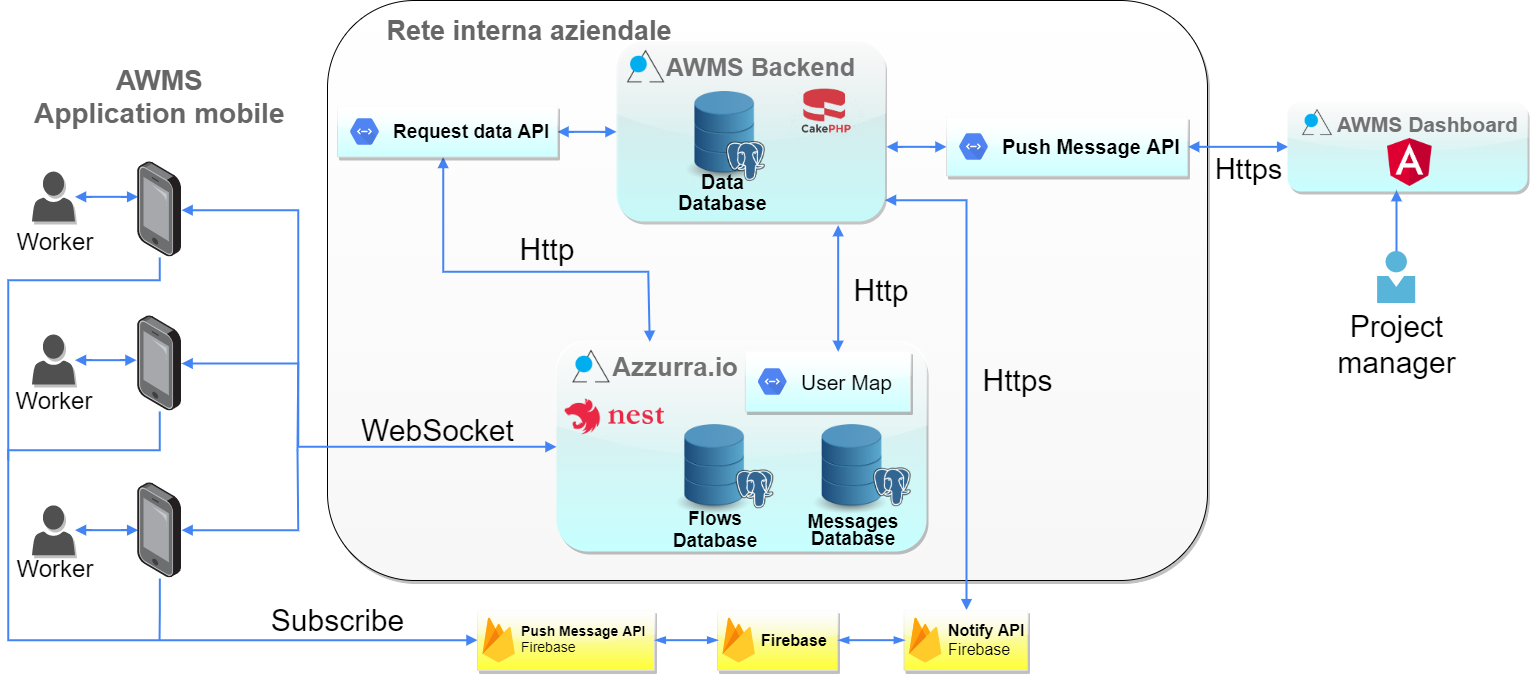
\includegraphics[scale=0.3]{AWMSDiagram.png}
 		\caption{Archittetura di sistema AWMS}
 		\label{fig:arch}
 	\end{center}
 \end{figure}

La figura precedente illustra come è composta l'architettura, e sono cosi descritte:
\begin{itemize}
	\item \textbf{AWMS Dashboard}:È il pannello di controllo attraverso il quale un project manager può interagire con la piattaforma AWMS per poter pianificare il lavoro da svolgere, cioè assegnare un compito alla persona più idonea. Il pannello di controllo è una applicazione web che è stata sviluppata in Angular. La dashboard per comunicare con il back-end, utilizza delle \gls{api}\ap{g} che il back-end espone, quindi per una ragione di sicurezza, back-end e l'applicazione web cioè il front-end, comunicano attraverso \gls{api}\ap{2} con in più l'utilizzo del protocollo di comunicazione HTTPS che cripta la comunicazione. Nella Figura ~\ref{fig:arch} viene mostrato il caso in cui il front-end utilizza \gls{api}\ap{3} per l'invio di notifiche push, questo perché è previsto che una volta il team leader sceglie il lavoratore più idoneo per un certo lavoro, il lavoratore deve essere avvisato, cosi sarà compito del front-end avvisare il back-end che c'è stata una nuova assegnazione e che questa assegnazione deve essere comunicata al diretto interessato attraverso un notifica sull'applicazione mobile con all'interno Azzurra.
\end{itemize}             % il mondo di AWMS
% !TEX encoding = UTF-8
% !TEX TS-program = pdflatex
% !TEX root = ../tesi.tex

%**************************************************************
\chapter{Azzurra Flow Engine}
\label{cap:flow engine}
%**************************************************************
\intro{Nel seguente capitolo verrà illustrato prima di tutto la struttura di un flusso conversazionale e successivamente il funzionamento del Azzurra Flow Engine la conseguente generazione dei messaggi da parte del \gls{bot}\ap{[g]} Azzurre e dell'utente umano}\\

%*************************************************************

\section{Cos'è}
Un elemento cardine dell'architettura di Azzurra è Azzurra Flow Engine. Esso è un motore conversazionale in grado di ricevere in input flussi conversazionali, implementati attraverso configurazioni JSON, che risiedono nel database di Azzurra.io. Essi vengono mandati in input a Azzurra Flow Engine quando il \gls{bot}\ap{[g]} Azzurra ne fa richiesta. Questi file sono codificati secondo una certa struttura fatta dai cosiddetti blocchi conversazionali e da altri campi che verranno illustrati in seguito. Tornando su Azzurra Flow Engine come scritto, riceve in input la configurazione JSON e grazie ai metodi che ha disposizione è in grado di interpretare i file JSON ricevuti e generare i messaggi che il \gls{bot}\ap{[g]} Azzurra deve fare visualizzare all'utente nella \emph{chat}.

\section{Flussi di conversazione}
I flussi di conversazione o conversazionali sono degli elementi fondamentali per la conversazione tra il \gls{bot}\ap{[g]} e l'utente umano. Essi sono delle configurazioni in JSON, dove ogni configurazione contiene un flusso di conversazione, e ogni flusso è un possibile ramo di conversazione che può essere fatto tra il \gls{bot}\ap{[g]} Azzurra e l'utente umano. Ogni configurazione contiene perciò dei particolari comandi che permettono al \gls{bot}\ap{[g]} di sapere quali messaggi deve mostrare all'utente umano e come comportarsi in base alle sue scelte. Ogni configurazione ha un id che contiene un codice univoco in modo tale da poter identificare ogni flusso di conversazione. Inoltre, l'esecuzione dei flussi di conversazione prevede che all'inizio ci sia l'esecuzione di un cosiddetto \emph{main flow}, in modo simile a come avviene per i programmi software, cioè c'è una funzione detta \emph{main} che viene eseguita per prima all'avvio del programma. Per indicare quale tra l'insieme dei flussi sia il \emph{main} si utilizza il campo isMainFlow dandogli il valore \emph{true}.
Oltre a questi campi esistono altri campi che sono:\\
\begin{itemize}
	\item \textbf{Shortcuts "shortcuts"};
	\item \textbf{Configurazione "config"};
	\item \textbf{Blocchi per la conversazione "blocks"}.
\end{itemize}
Tutti e tre verranno illustrati nelle seguenti sottosezioni.
\subsection{Shortcuts “shortcuts”}
Il campo shortcuts è il campo dedicato per le cosiddette "scorciatoie" cioè, tra le funzionalità che il \gls{bot}\ap{[g]} offre all'utente c'è anche la possibilità di visualizzare un menu dove vengono mostrate tutte le funzionalità offerte dal \gls{bot}\ap{[g]} e scegliere direttamente quelle eseguire in ogni momento.

\begin{figure}[htbp]
	\centering
	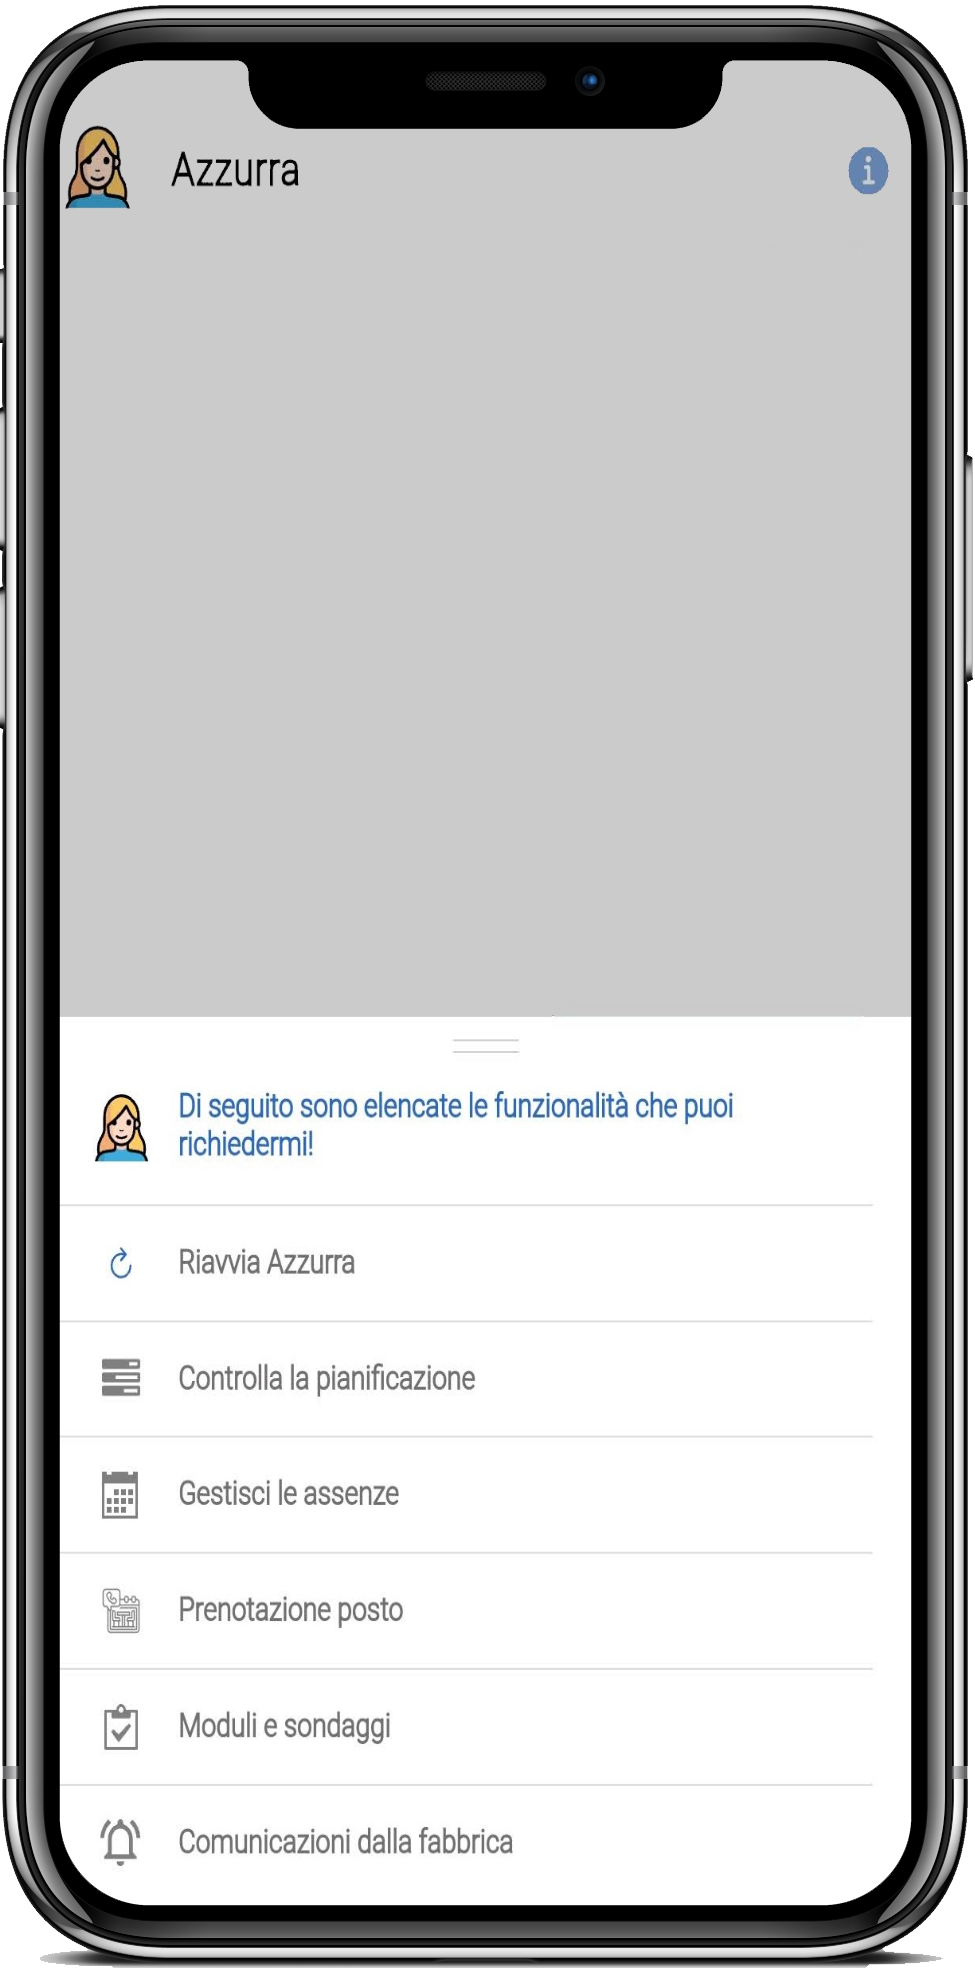
\includegraphics[scale=0.2]{shortcuts.png}
	\caption{Menu contenente le shortcuts disponibili}
\end{figure}

Il campo shortcuts viene indicato nel file con la \emph{keyword} shortcuts
e al suo interno contiene i seguenti campi:
\begin{itemize}
	\item text: È un campo che può essere di tipo \emph{string} e quindi contiene il testo da far visualizzare nel bottone della scorciatoia all'utente, oppure un oggetto che contiene un attributo per ogni lingua disponibile, dove ogni attributo ha il testo nella lingua straniera che l'attributo rappresenta. Il testo nella lingua di default (italiano) è contenuto nell’attributo “default” ;
	\item flowId: Contiene l'identificativo del flusso che la scorciatoia permette di far eseguire;
	\item icon: Per rendere la UI più accattivante è possibile aggiungere al bottone dedicato alla scorciatoia, delle icone per ogni scorciatoia.
\end{itemize}
\clearpage
\subsection{Configurazione "config"}
Il campo config permette di indicare attraverso il campo startBlockId quale blocco di conversazione del flusso deve essere eseguito per primo, per tale campo ci sarà il codice identificativo del primo blocco da eseguire. Il campo configurazione viene indicato nel file con la \emph{keyword} config.

\subsection{Blocchi per la conversazione "blocks"}
Il campo Blocchi indicato nel file con la \emph{keyword} blocks contiene tutti i blocchi per la conversazione i quali indicano i messaggi che devono essere mostrati e i passi da eseguire a seconda delle scelte inserite dell'utente umano.
I blocchi utilizzati per la conversazione si differenziano tra lo loro dal tipo di blocco a cui appartengono. Ogni tipo ha proprie caratteristiche uniche ma anche delle caratteristiche comuni, questo perché tutti i tipi di blocchi per la conversazione ereditano da un tipo padre detto BLOCK. I tipi figli di Block sono i seguenti:
\begin{itemize}
	\item\textbf{ASK};
	\item\textbf{SAY};
	\item\textbf{IF};
	\item\textbf{PROC};
	\item\textbf{JUMP};
	\item\textbf{CALLFUNC}.
\end{itemize}
Di seguito verrà illustrata la struttura e il ruolo di BLOCK e dei suoi figli.
\subsubsection{BLOCK}

BLOCK è il blocco di conversazione attraverso il quale tutti blocchi ereditano delle caratteristiche comuni della sua struttura, di fatto BLOCK non può essere utilizzato e, quindi, può essere paragonato a una classe astratta nell’ambito della programmazione ad oggetti, dove vengono definite delle caratteristiche della classe ma non può essere istanziata, perciò può essere solo ereditata dai suoi figli, che diventano classi concrete istanziabili.

%\begin{figure}[htbp]
%	\centering
%	\includegraphics[height=5cm]{img/block.png}
%	\caption{Definizione della classe BLOCK}
%\end{figure}

Ha la seguente struttura:

\begin{itemize}
	\item \textbf{id}: È un campo di tipo \emph{string} che identifica univocamente il blocco tra un insieme di blocchi di conversazione;
	\item \textbf{type}: Questo campo indica il tipo di blocco che come scritto può essere di tipo ASK
	 o SAY o IF o PROC o JUMP oppure CALLFUNC;        
	\item \textbf{text}: È un campo che può essere di tipo \emph{string} contente il testo da far visualizzare all'utente, oppure un oggetto che contiene un attributo per ogni lingua disponibile contente del testo nella corrispondente lingua, e un attributo default che contiene il testo di default;
	\item \textbf{variations}: Anch'esso è un tipo \emph{string} che contiene uno o più testi alternati al principale rappresentato dal campo text. Il funzionamento prevede che randomicamente il testo da mostrare all'utente non sarà quello principale ma uno delle alternative contenuto all'interno di variations, verrà perciò scelto in modo casuale, uno dei testi a disposizione; 
	\item \textbf{target}: Questo campo contiene l'id del prossimo blocco di conversazione da eseguire;
	\item \textbf{variable}: Questo campo indica il nome della variabile “conversazionale” su cui salvare eventuali valori di input inseriti dall’utente: il flow engine quindi, attraverso dei metodi specifici, ha la capacità di salvare tutte le scelte fatte dell’utente, memorizzandole nelle variabili indicate nel campo variable.
	\item \textbf{widget}: Indica il tipo di oggetto grafico detto Widget che deve essere utilizzato a supporto del blocco, esistono i seguenti tipi di Widget che verranno descritti successivamente:
	\begin{itemize}
		\item \textbf{BUTTONS};
		\item \textbf{ITEMS};
		\item \textbf{PICKER};
		\item \textbf{TIMEPICKER};
		\item \textbf{DATEPICKER};
		\item \textbf{CALENDAR};
		\item \textbf{QRSCANNER}.
	\end{itemize}
	\item \textbf{widgetOptions}:Permette di aggiungere delle opzioni in più al Widget, per esempio permette di indicare del testo all'interno dei Widget oppure indicare il valore minimo accettabile.
\end{itemize} 


\subsubsection{ASK}
Il blocco di conversazione ASK ha la funzione di mostrare all’utente una serie di opzioni disponibili e chiedere quali tra queste vuole eseguire. Quindi mostra le possibili scelte rimanendo in attesa di una risposta dell’utente. Infine esegue il comando collegato alla scelta effettuata dall’utente dirottando la conversazione al blocco successivo. 

\begin{figure}[htbp]
	\centering
	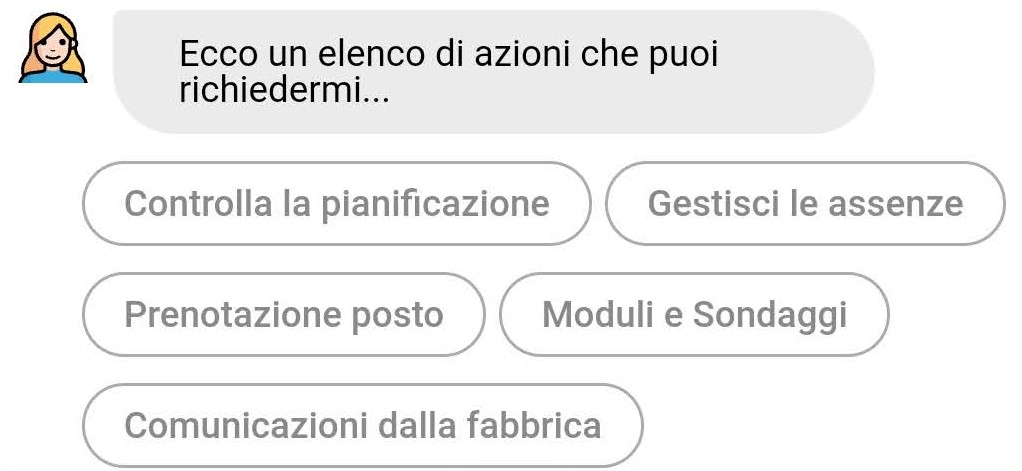
\includegraphics[scale=0.25] {blockItems.jpg}
	\caption{Esempio di messaggio prodotto da un blocco di tipo ASK}
\end{figure}

Oltre a campi del tipo BLOCK ha i seguenti campi in più:

\begin{itemize}
	\item \textbf{category}: Il blocco ASK è ulteriormente distinguibile in ASK o in MENU che si differenziano nel seguente aspetto:\\
	nel caso sia di categoria ASK tutte le opzioni disponibili portano a un blocco di conversazione successivo diverso mentre per MENU tutte le opzioni portano tutte allo stesso blocco;
	\item \textbf{source}: Parametro che contiene il nome di una variabile a cui fare riferimento per prendere i dati da utilizzare. Se non si fa riferimento a nessuna variabile allora va settato a \emph{NULL};
	\item \textbf{items}: Questo campo contiene un array d'oggetti di tipo BlockItem che rappresentano le possibili scelte che può fare l'utente, essi graficamente vengono rappresentati come dei pulsanti;
	\item \textbf{sourceType}: Parametro che indica la modalità di utilizzo della variabile contenuta nel campo source;
	Sono previste due modalità:
	\begin{itemize}
		\item \textbf{LIST}: In questo caso la variabile contenuta in source viene ignorata e vengono presi tutti gli oggetti di tipo BlockItem contenuti nel campo items che vengono trasformati in bottoni da far visualizzare a video;
		\item \textbf{VARIABLE}: In questo caso tutto ciò che è contenuto nella variabile del campo source viene trasformato in bottoni da far visualizzare a video, per poterlo fare devono essere formattati in una struttura del tipo chiave valore.
	\end{itemize}	
\end{itemize} 

\subsubsection{SAY}

Il blocco di conversazione SAY ha la funzione di mostrare all'utente un messaggio a video attraverso il quale si comunica l'esito della operazione precedente e il risultato da essa ricavata. Perciò l'utente richiede l'esecuzione di una qualche operazione, viene eseguita e una volta conclusa il \gls{bot}\ap{[g]} risponderà all'utente con il risultato ricavato precedentemente.

\begin{figure}[htbp]
	\centering
	
\includegraphics[scale=0.25]{say.jpg}
	\caption{Esempio di messaggio prodotto da un blocco di tipo SAY}
\end{figure}
Oltre a campi del tipo BLOCK ha il seguente campo in più:

\begin{itemize}
	\item \textbf{attachments}: Campo che contiene un array d'oggetti di tipo BlockAttachment che permettono di allegare immagini o file PDF.
\end{itemize}

Inoltre sono presenti i campi items, source e sourceType, con analogo funzionamento del blocco ASK per inserire eventuali bottoni che aprono schede o link contenenti il risultato richiesto.

\subsubsection{IF}

Il blocco di conversazione IF ha la funzione di verificare se una o più condizioni sono rispettate. Perciò verifica se le condizioni sono soddisfatte, e in base all'esito verrà scelto il prossimo blocco da eseguire.

%\begin{figure}[htbp]
%	\centering
%	\includegraphics[scale=1]{img/if.png}
%	\caption{Definizione della classe IF}
%\end{figure}
Oltre a campi del tipo BLOCK ha i seguenti campi in più:

\begin{itemize}
	\item \textbf{conditions}: Contiene una o più condizioni che devono essere verificate;
	\item \textbf{trueBlockTarget}: Indica il blocco successivo da eseguire se le condizioni sono soddisfate;
	\item \textbf{falseBlockTarget}: Indica il blocco successivo da eseguire se le condizioni non sono soddisfate.
\end{itemize}


\subsubsection{PROC}
Il blocco di conversazione PROC permette di eseguire delle operazioni sulle variabili conversazionali cioè, assegnazione o trasformazione dei dati. Ad esempio, permette di riordinare i dati ricevuti dal server in modo da poter essere utilizzati dai source con sourceType uguale a VARIABLE.

%\begin{figure}[htbp]
%	\centering
%	\includegraphics[scale=1]{img/proc.png}
%	\caption{Definizione della classe PROC}
%\end{figure}

Oltre a campi del tipo BLOCK ha il seguente campo in più:

\begin{itemize}
	\item \textbf{expressions}: Contiene le espressioni da eseguire, ad esempio, per la formattazione dei dati.
	Ha i seguenti campi:
	\begin{itemize}
		\item \textbf{var}: Contiene il nome della variabile dove viene salvato il risultato della formattazione;
		\item \textbf{type}: Indica il tipo di formattazione che si vuole applicare, al momento c'è solo una formattazione disponibile:
		\begin{itemize}
			\item \textbf{reduce to textvalue}: Permette di riordinare i vari valori che si hanno in una struttura chiave valore.
		\end{itemize}
		\item \textbf{args}: Contiene un espressione in Handlebars, un linguaggio di \emph{templating} utilizzato per costruire \emph{template} in HTML con dei cosiddetti segnaposto che verranno poi valorizzati con dei valori, utilizzando delle \emph{keyword} del linguaggio, in modo da ottenere delle componenti in HTML da mostrare come messaggio.
	\end{itemize}
\end{itemize}

\subsubsection{JUMP}

Il blocco di conversazione JUMP permette di cambiare il flusso conversazionale ed eseguirne una altro. In termini tecnici si passa da un JSON di configurazione ad un altro dove ogni configurazioni in JSON contiene un specifico flusso di conversazione. Perciò, grazie a JUMP si può "saltare" da un flusso di conversazione a un altro.Il blocco di conversazione JUMP permette di cambiare il flusso conversazionale ed eseguirne un altro. In termini tecnici si passa da un JSON di configurazione ad un altro dove ogni configurazione in JSON contiene un specifico flusso di conversazione. Perciò, grazie a JUMP, si può "saltare" da un flusso di conversazione ad un altro.
Nel campo target in questo caso non viene indicato l’id del blocco successivo ma, l’id del \emph{flow} che si vuole eseguire.


%\begin{figure}[htbp]
%	\centering
%	\includegraphics[height=5cm]{img/jump.png}
%	\caption{Definizione della classe JUMP}
%\end{figure}


\subsubsection{CALLFUNC}

Il blocco di conversazione CALLFUNC è il blocco attraverso il quale, il \gls{bot}\ap{[g]} (l'applicazione mobile) può richiedere l’esecuzione di chiamate ad \gls{api}\ap{[g]} (interne o esterne). Attraverso un \gls{WebSocket}\ap{[g]}, che mantiene una connessione tra il \gls{bot}\ap{[g]} e Azzurra.io, quest’ultima richiama, a sua volta, delle \gls{api}\ap{[g]} di \gls{AWMS}\ap{[g]} (o esterne ad \gls{AWMS}\ap{[g]}) per ottenere i dati richiesti dell’utente o per salvare dati. 

%\begin{figure}[htbp]
%	\centering
%	\includegraphics[scale=1]{img/callfun.png}
%	\caption{Definizione della classe CALLFUNC}
%\end{figure}

Oltre a campi del tipo BLOCK ha il seguente campo in più:

\begin{itemize}
	\item \textbf{payload}: Campo che contiene l'intestazione e il corpo della richiesta verso Azzurra.io;
	Contiene i seguenti campi:
	\begin{itemize}
		\item \textbf{type}: Indica se la chiamata è verso Azzurra.io attraverso il valore \textsf{int} oppure verso un servizio esterno con il valore \textsf{ext}.
	\end{itemize}
	Se la chiamata è di tipo int ha la seguente struttura:
	\begin{itemize}
		\item \textbf{route}: Indica il metodo di Azzurra.io da richiamare;
		\item \textbf{body}: Contiene il corpo della richiesta, nello specifico un \emph{template} costruito da Handlebars che verrà idratato da Azzurra.io nel caso sia una richiesta di dati o dal \gls{bot}\ap{[g]} nel caso in cui debba inviare dei dati da salvare.
	\end{itemize}
	Se la chiamata è di tipo ext ha la seguente struttura:
	\begin{itemize}
		\item \textbf{config}: Contiene la struttura di una chiamata HTTP.\\
		Ha i seguenti campi:
		\begin{itemize}
			\item \textbf{url}: Contiene l'indirizzo URL del servizio esterno a cui fare richiesta;
			\item \textbf{method}: Se la richiesta e di tipo GET o POST;
			\item \textbf{headers}: Contiene l'intestazione per la richiesta HTTP;
			\item \textbf{params}: Contiene le variabili necessarie per la chiamata, questo campo viene usato solo se la richiesta e di tipo GET;
			\item \textbf{data}: Analogo al campo params solo se viene usato dai metodi POST.
		\end{itemize}
	\end{itemize}
	\item \textbf{var}: Indica il nome della variabile dove salvare il risultato della richiesta;
	\item \textbf{failureBlockTarget}: Indica il blocco successivo da eseguire se la richiesta non va a buon fine;
	\item \textbf{successBlockTarget}: Indica il blocco successivo da eseguire se la richiesta va a buon fine.
\end{itemize}

\subsection{Oggetti ausiliari}
Come scritto nella sezione precedente questi oggetti vengono definiti per essere utilizzati all’interno dei blocchi per svolgere un azione di supporto, affinché si possa raggiungere ciò per cui sono stati realizzati i blocchi di conversazione stessi.\\
Di seguito vengono indicate tutte le classi degli oggetti ausiliari disponibili.

\subsubsection*{Widget}
È un oggetto che a seconda del tipo permette di realizzare delle componenti grafiche, esso viene utilizzo per richiedere delle azioni da parte dell’utente umano.
Ha i seguenti tipi:
\begin{itemize}
	\item \textbf{BUTTONS}: Genera dei bottoni arrotondati;
	\begin{figure}[h]
		\centering
		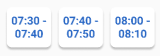
\includegraphics[scale=1.1]{buttons.png}
	\caption{Rappresentazione grafica dei buttons}
	\end{figure}
	\clearpage
	\item \textbf{ITEMS}: Genera dei bottoni quadrati;
	\begin{figure}[h]
		\centering
		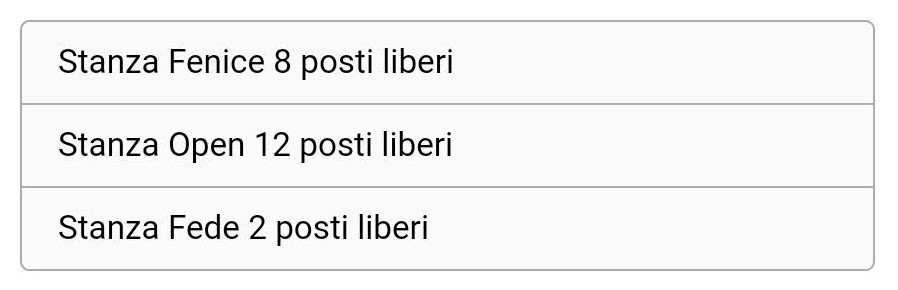
\includegraphics[scale=0.3]{items.jpg}
		\caption{Rappresentazione grafica degli items}
	\end{figure}
	\item \textbf{PICKER}: Genera, attraverso il componente “ion-picker” di \textsf{Ionic} una finestra di dialogo dove si può selezionare una opzione tra quelle proposte;
	\begin{figure}[h]
		\centering
		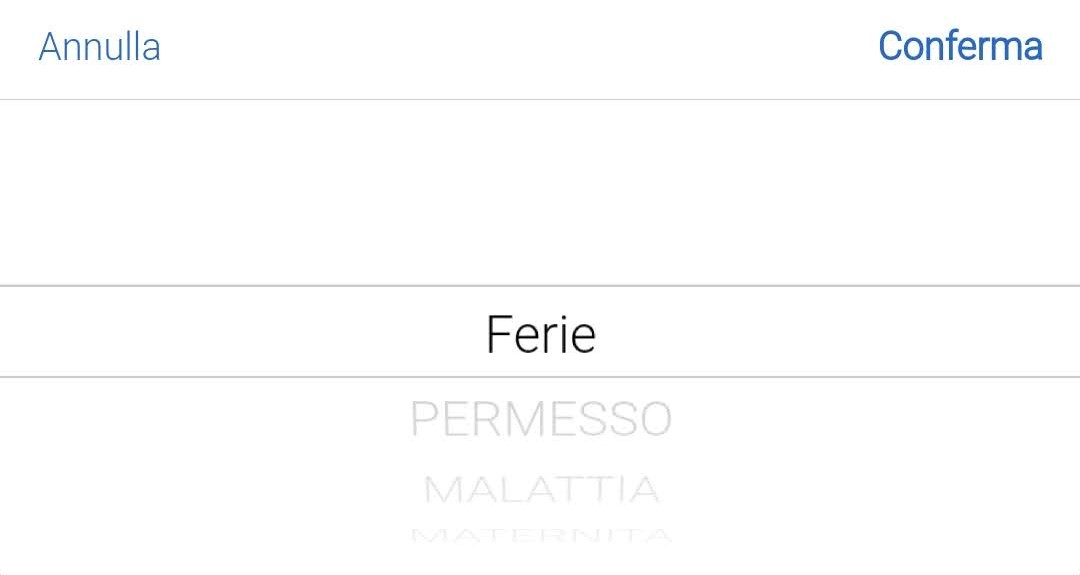
\includegraphics[scale=0.2]{picker.jpg}
		\caption{Rappresentazione grafica del picker}
	\end{figure}
	\item \textbf{TIMEPICKER}: Analogo al PICKER solo che le opzioni da scegliere è l'orario che si vuole selezionare;
	\begin{figure}[h]
		\centering
		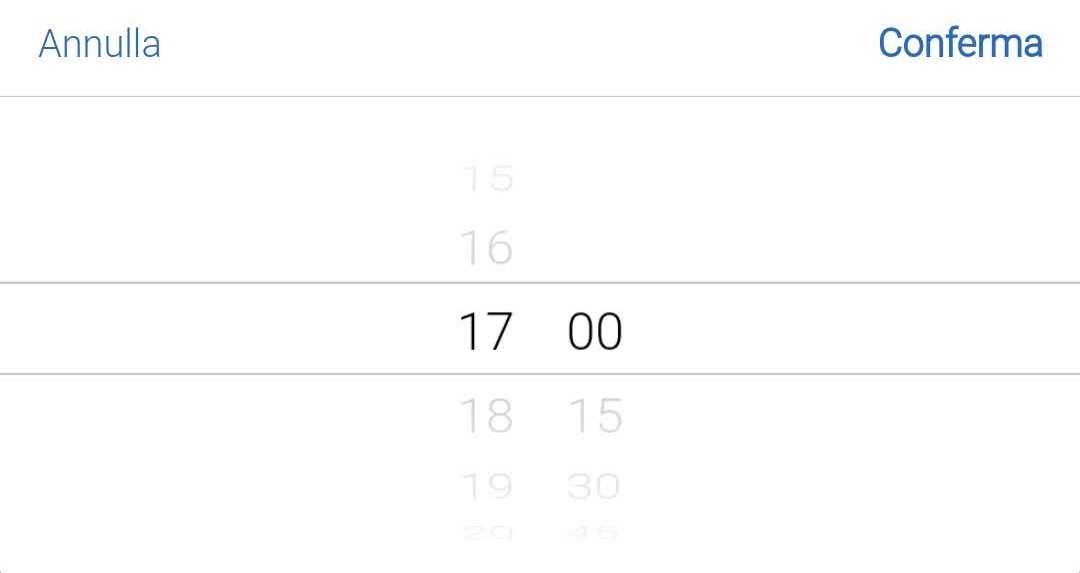
\includegraphics[scale=0.2]{timePicker.jpg}
		\caption{Rappresentazione grafica del time picker}\label{fig:time}
	\end{figure}
\clearpage
	\item \textbf{DATEPICKER}: Analogo al PICKER solo che le opzioni da scegliere è la data che si vuole selezionare;
	\begin{figure}[h]
		\centering
		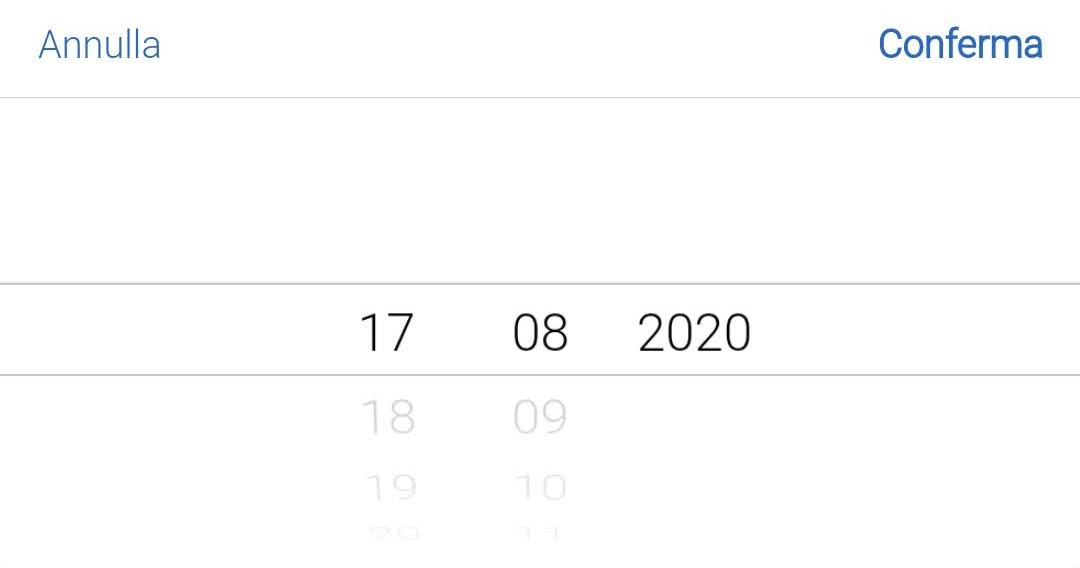
\includegraphics[scale=0.2]{datePicker.jpg}
		\caption{Rappresentazione grafica del date picker}\label{fig:date}
	\end{figure}
	\item \textbf{CALENDAR}: Fa comparire un calendario grazie all'utilizzo del plugin Calendar per Ionic;
	\item \textbf{QRSCANNER}: Permette di accedere alla fotocamera (solo se si hanno i permessi) e di decodificare i codici QR-code tutto ciò grazie al plugin QR Scanner di Cordova.
	\begin{figure}[h]
		\centering
		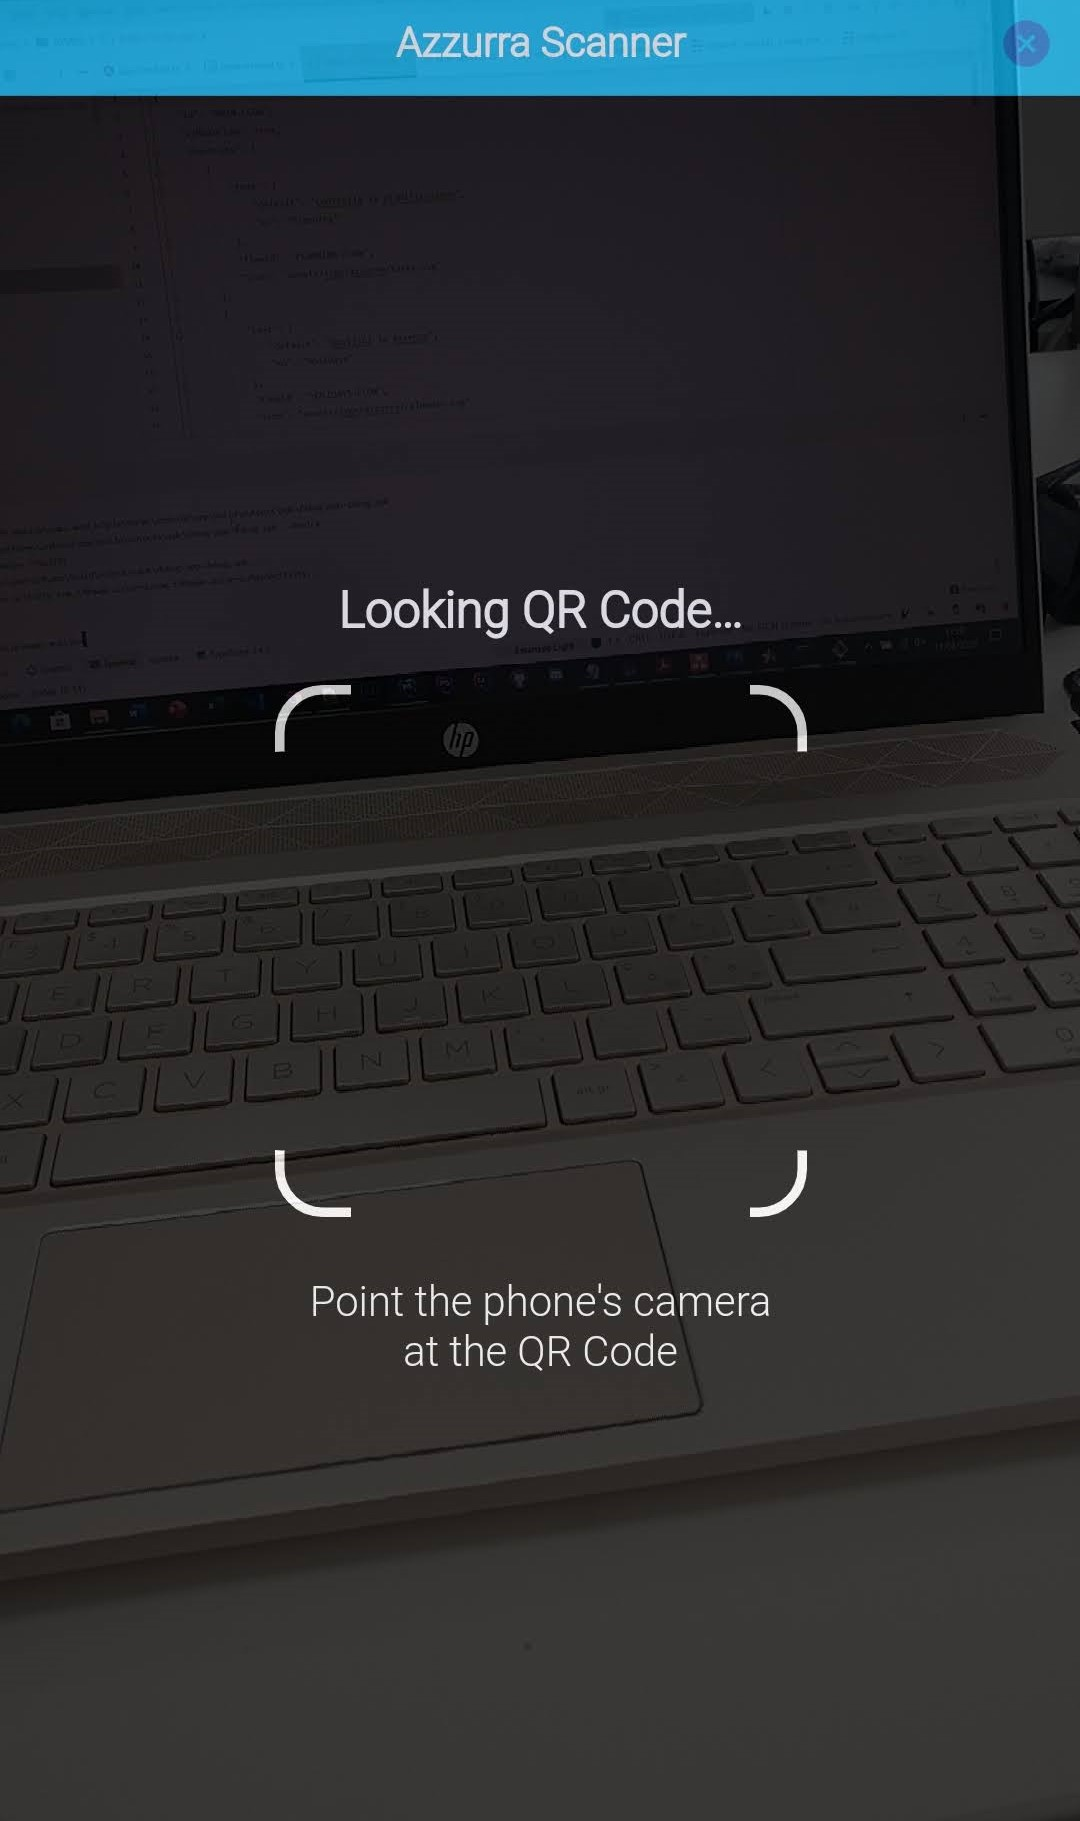
\includegraphics[scale=0.2]{qrcode.jpg}
		\caption{Rappresentazione grafica del QR scanner}\label{fig:qrc}
	\end{figure}
\end{itemize}

\subsubsection*{BlockItem}
Questo oggetto rappresenta una possibile scelta che può fare l'utente, graficamente viene rappresentato come un bottone cliccabile dall'utente.

\begin{figure}[h]
	\centering
	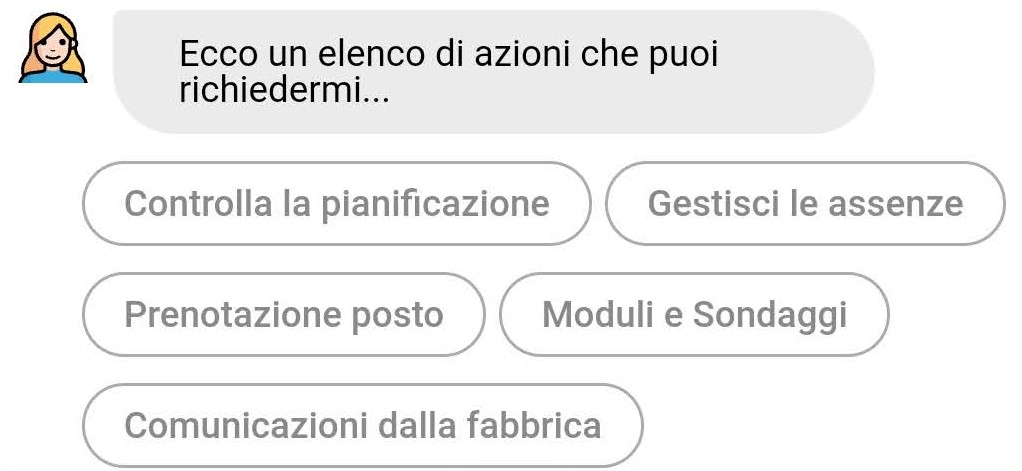
\includegraphics[scale=0.3]{blockItems.jpg}
	\caption{Rappresentazione grafica del BlockItem}
\end{figure}
Ha la seguente struttura:

\begin{itemize}
	\item \textbf{text}: Contiene l'etichetta che viene visualizzata sul bottone;
	\item \textbf{target}: Contiene l'id del prossimo blocco da eseguire.
\end{itemize}



\subsubsection*{BlockAttachment} 
L'oggetto in esame permette di allegare immagini o file PDF da mostrare all'utente.

Ha la seguente struttura:

\begin{itemize}
	\item \textbf{id}: Contine un codice univoco che identifica ogni BlockAttachment;
	\item \textbf{type}: Indica se contiene un PDF o una immagine, nel caso di un'immagine indica se è in formato JPG o in JPEG oppure in PNG.
\end{itemize}	

\section{Gestione dell'internazionalizzazione di AWMS}
Per il sistema \gls{AWMS}\ap{[g]} è stata implementata la gestione dell'\gls{i18n}. Infatti per rendere tutto il sistema, sia lato backend sia lato Azzurra, adattabile a più lingue, sono stati definiti un insieme di testi multi-lingua. Per gestire questi testi multi-lingua è stato progettato di utilizzare un \emph{template engine} al fine di ottenere la parametrizzazione dei testi. \\
Un \emph{template engine} non è altro che un programma che prevede la definizione di blocchi detti \emph{template} spesso scritti in HTML, che hanno la caratteristica di avere dei segnaposto detti \emph{placeholders}, che vengono sostituiti dai dati da visualizzare. In questi blocchi perciò  viene definito il testo scritto in una specifica lingua e in quali punti del testo devono essere inseriti i dati per la visualizzazione. Per la sostituzione dei \emph{placeholders} solitamente il \emph{template engine} utilizza file JSON, in cui i segnaposti sono solitamente rappresentati dai campi che compongono l’oggetto salvato nel file JSON, i quali andranno a sostituire i segnaposti con i loro valori che rappresentano i dati da visualizzare. Quindi il \emph{template engine} definisce dei template che vengono "idratati" cioè, vengono sostituiti i \emph{placeholders} con dati veri. Chiaramente i \emph{template} vengono riutilizzanti anche se i dati visualizzati variano. Vengono perciò definiti \emph{template} di testi "localizzati" cioè scritti in un delle lingue supportate dal sistema \gls{AWMS}\ap{[g]}.\\
 Un \emph{template engine} può essere facilmente implementato in JavaScript ma come scelta progettuale di è stato deciso di utilizzare \emph{Handlebars}. \emph{Handlebars} è un estensione del \emph{template engine} \emph{mustache} perché, per indicare i \emph{placehorders} all'interno dei \emph{template} utilizza le doppie parentesi graffe le quali racchiudono la parola da sostituire. È stato scelto di utilizzare \emph{Handlebars} perché garantisce delle performance migliori infatti, permette di compilare i \emph{template}, riducendo il tempo di \emph{rendering} quando un blocco di codice viene creato più di una volta. Inoltre \emph{Handlebars} permette di utilizzare i cosiddetti "Helpers" che permettono l'esecuzione di funzionalità che vanno a manipolare la formattazione del testo. Infine, un’altra caratteristica avanzata di \emph{Handlebars} è il supporto ai "Partials". Con tale termine si indica la possibilità di innestare \emph{template} l’uno dentro l’altro, permettendone la riusabilità e la realizzazione di codice più ordinato.\\
 
 Nel lato backend ciascun testo "localizzato" è persistito in apposite tabelle di un \emph{database}.\\
 
 Nel lato \gls{bot}\ap{[g]} Azzurra come spiegato in precedenza, nel campo text dei blocchi conversazionali, c'è un oggetto che contiene un attributo per ogni lingua disponibile contente del testo nella corrispondente lingua, e un attributo default che contiene il testo di default. Quindi Il flow engine, interpretando ciascun blocco conversazionale, effettua un processamento dei testi scegliendo, se presenti, quelli relativi alla lingua dell'utente.\\
 
 Durante lo stage un parte del tempo è stata dedicata allo studio di \emph{Handlebars} e alla scrittura dei \emph{template} che in molti casi, richiedevano l'inserimento dei \emph{placeholders } con la sintassi \emph{mustache}.
 

\section{Funzionamento di Azzurra Flow Engine}
L'Azzurra Flow Engine è l'elemento in grado di interpretare i dati contenuti nelle configurazioni JSON. Grazie a esso è possibile eseguire il corretto flusso della conversazione e generare i messaggi da mostrare nella \emph{chat} dell'applicazione mobile. 
\subsection{Messaggio del bot Azzurra}
Per implementare le funzionalità del Azzura Flow Engine vengono utilizzate le seguenti classi sviluppate in Angular:
\begin{itemize}
	\item \textbf{FlowService}: Ha i metodi necessari per interpretare le configurazioni JSON e quindi, per poter sapere quale tipo di messaggio deve essere costruito, ricavare i dati necessari per costruire i messaggi e sapere come procedere con la conversazione;
	\item \textbf{AzzurraService}: Permette principalmente di fare da tramite tra il FlowService e il \textbf{ChatComponent} per la creazione della conversazione. Oltre a ciò permette di gestire operazioni ad alto livello come il caricamento dei messaggi precedenti nella \emph{chat} e gestire le notifiche che possono arrivare dalla \emph{dashboard};
	\item \textbf{ChatComponent}: Si occupa di far visualizzare i messaggi della conversazione;
	\item \textbf{ChatService}: Ha il compito di creare e gestire i Widget da aggiungere al messaggio da mostrare, e inoltre, di ricavarne da essi le risposte dell'utente umano.
\end{itemize}

\begin{figure}[htbp]
	\centering
	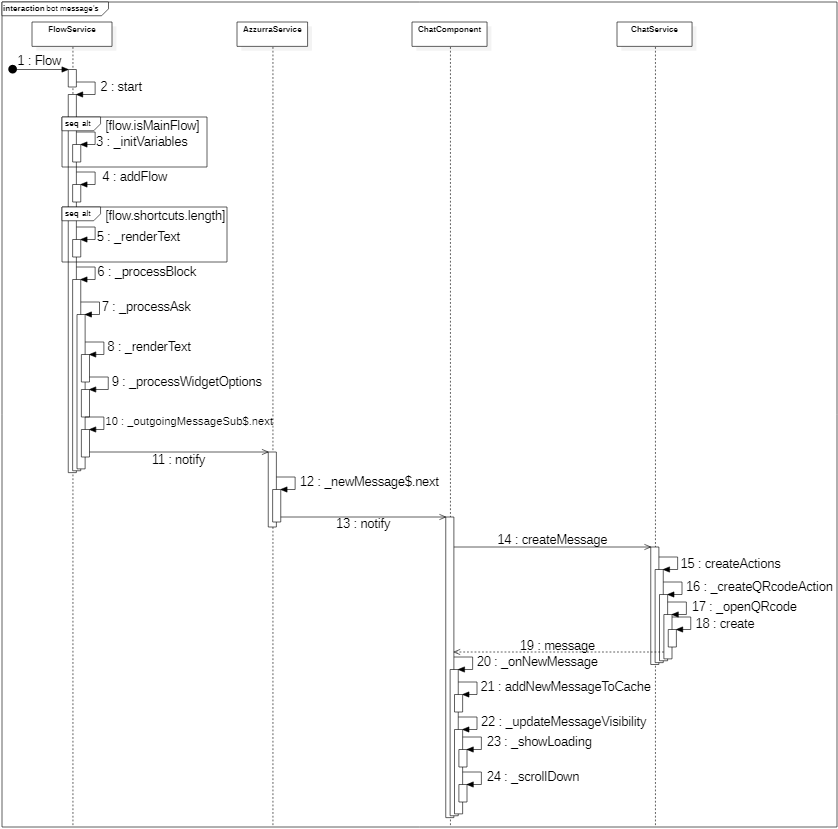
\includegraphics[height=20cm, width=14cm]{sd_bot_mx2.png}
	\caption{Diagramma di sequenza del processo di generazione del messaggio del bot Azzurra}\label{fig:mxBot}
\end{figure}

Una volta che si è stabilità la connessione con Azzurra.io, attraverso un \gls{WebSocket}\ap{[g]}, inizializzato il Flow Engine e infine, ricevuto la configurazione JSON contenente il flusso conversazionale, la generazione di un messaggio da parte del \gls{bot}\ap{[g]} Azzurra prevede i seguenti passi:\\
\begin{enumerate}
	\item Viene inviato all’applicazione mobile il flusso conversazionale richiesto precedentemente;
	\item Viene avviato nel FlowService il metodo start(), il quale riceve in input il flusso da eseguire. Viene verificato se il flusso ricevuto risulta essere il \emph{main flow}, in questo caso vengono inizializzate le variabili conversazionali d'ambiente utilizzate come supporto per la generazione dei messaggi, ad esempio esiste una variabile d'ambiente per indicare il giorno corrente o il formato della data da utilizzare;
	\item Una volta impostate le variabili conversazionali d’ambiente e usciti dal blocco condizionale viene salvato il flow da eseguire attraverso il metodo \_addFlow() che imposta come flusso corrente da eseguire il flusso ricevuto in input. Viene infine controllato se la configurazione definisce delle eventuali shortcuts;
	\item Se ci sono delle shortcuts viene chiamato il metodo \_renderText() per crearle, esso sarà in grado di interpretare il pezzo di configurazione dove sono definite le proprietà di ogni shortcuts;
	
	Una volta finita l'esecuzione del metodo, l'esecuzione torna al metodo start().
	\item Sempre in start() viene chiamata l'esecuzione di \_processBlock() dandogli in input il primo blocco del flusso da eseguire
	
	\item Nel metodo \_processBlock() viene eseguito il blocco che riceve in input, in questo caso il blocco da eseguire è il primo blocco del flusso come detto nel punto precedente. In questo metodo si verifica innanzitutto se c'è un blocco da eseguire, se non c'è viene emesso un segnale che informa che il flusso di conversazione è terminato, mentre se c'è un blocco allora si imposta questo blocco come quello in esecuzione e si verifica di che tipo è il blocco.\\
	A seconda del tipo del blocco vengono eseguite le seguenti istruzioni:
	\begin{itemize}
		\item \textbf{Caso SAY}: Viene eseguito il metodo \_processSay() ricevendo in input il blocco corrente. Il metodo prende il valore salvato nel campo text e le eventuali variations del blocco, generando il testo del messaggio da mostrare attraverso il metodo \_renderText(). Vengono generati eventuali BlockItems attraverso il metodo \_buildSayItems() il quale controlla il sourceType e in base al valore che ha, genera i BlockItems. Tornando in \_processSay(), se presenti vengono anche eseguite le widgetOptions attraverso il metodo \_processWidgetOptions() e creati gli eventuali BlockAttachments. Infine, viene emesso il nuovo messaggio creato per il \gls{bot}\ap{[g]} Azzurra e si passa all'esecuzione del prossimo blocco;
		\item \textbf{Caso ASK}: Viene eseguito il metodo \_processAsk ricevendo in input il blocco corrente. Il metodo salva il nome della variabile contenuta nel campo var, che contiene la risposta dell'utente. Analogamente per quanto accede per il blocco SAY viene creato il testo della domanda e attraverso il metodo \_buildQuestions() vengono creati i BlockItems delle possibili scelte. Inoltre, vengono processati gli eventuali widgetOptions. Infine, viene emesso il nuovo messaggio creato per il bot, il quale rimane in attesa della risposta dell'utente umano quando verrà visualizzato il messaggio;
		\item \textbf{Caso JUMP}: Viene eseguito il metodo \_processJump() ricevendo in input il blocco corrente. Richiama il metodo \_getFlow() pasandogli l'identificativo del flusso da eseguire attraverso il campo target. Il metodo citato richiede ad Azzurra.io il flusso che ha l'identificativo uguale a quello ricevuto in input, e una volta ricevuto comincia l'esecuzione del nuovo flusso conversazionale richiamando start();
		\item \textbf{Caso IF}: Viene eseguito il metodo \_processIf() passando in input il blocco corrente. Valuta la condizione attraverso \_manageConditions(), e in base al risultato stabilisce quale sarà il blocco di conversazione successivo da eseguire;
		\item \textbf{Caso PROD}: Viene eseguito il metodo \_processProd() passandogli in input il blocco corrente. Stabilisce che formattazione deve essere fatta e la esegue attraverso il metodo \_manageExpressions(). Infine, passa all'esecuzione del prossimo blocco;
		\item \textbf{CALLFUNC}: Viene ricavato il \emph{payload} del blocco e codificato il \emph{template} in Handlebars per generare il corpo della richiesta, una volta fatto ciò la richiesta è pronta e viene mandata a Azzurra.io. Successivamente viene salvata la risposta sulla variabile indicata del campo var e in base alla risposta, se andata a buon fine oppure no, si eseguirà il corrispondente blocco successivo.
	\end{itemize}	
	\item Nella Figura~\ref{fig:mxBot} viene mostrato il caso in cui viene eseguito il metodo \_processAsk() perché il blocco attuale e di tipo ASK;
	\item Viene eseguito \_renderText() per costruire il testo della domanda;
	\item Attraverso \_buildQuestions() vengono creati i BlockItems delle possibili scelte;
	\item Viene eseguito il metodo \_processWidgetOptions() per creare le eventuali widgetOptions;
	\item A questo punto la struttura del messaggio è stata creata, manca solo la visualizzazione nella \emph{chat} che è compito di ChatComponent, perciò attraverso il metodo next() di Angular, viene emesso un segnale che avvisa chi è in ascolto su \_outgoingMessageSub\$ che è stato creato un nuovo messaggio e che occorre visualizzarlo;
	\item Viene notificato agli ascoltatori l'evento descritto al punto precedente;
	\item Nel AzzuraService c'è un ascoltatore che riceve i segnali mandati dai metodi di FlowService, perciò con la notifica inviata al punto precedente AzzuraService ha il messaggio che è stato appena creato;
	\item AzzuraService emettere a sua volta il nuovo messaggio appena ricevuto, verso l'ascoltatore presente in ChatComponent;
	\item Quando ChatComponent riceve il messaggio eseguirà il metodo createMessage() di ChatService passandogli il messaggio ricevuto. Questo metodo si occuperà di far creare il messaggio grafico nel modo corretto.
	Innanzitutto, verifica chi ha emesso il messaggio, se è stato l'utente umano o il \gls{bot}\ap{[g]} Azzurra. Nel caso in cui il messaggio sia del \gls{bot}\ap{[g]} Azzurra viene indicato il testo da mostrare estraendolo dal messaggio ricevuto in input e aggiunto lo sprite di Azzurra per indicare graficamente che il messaggio viene dal bot;
	\item Nel caso in cui il messaggio preveda delle azioni da parte dell'utente umano, ovvero ci siano dei Widget, viene chiamato il metodo createAction() passandogli sempre il messaggio. In questo metodo viene verificato che tipo di Widget deve essere creato, per ogni Widget c'è un corrispondente metodo che ne imposta il testo da far visualizzare quando l'utente interagisce con esso, tale testo potrebbe essere un testo di default o un testo indicato nel campo widgetOptions inoltre nel caso del DATEPICKER o TIMEPICKER, viene impostato il formato di visualizzazione del giorno e dell'ora;
	\item Nel caso rappresentato dalla Figura~\ref{fig:mxBot}, viene chiamato il metodo \_createQRcodeAction()
	 il quale imposta il testo da mostrare e chiama il metodo \_openQRcode();
	\item \_openQRcode() Richiama il metodo create() per creare e aprire il Widget QRCODE;
	\item In \_openQRcode() viene chiamato il metodo create() che permette di utilizzare il ModalController di Ionic il quale crea una nuova finestra grafica con dentro la classe che gestisce il lettore di \gls{QR code}\ap{[g]}. Si crea quindi graficamente il Widget. I corrispondenti metodi \emph{open} per DATEPICKER e TIMEPICKER non utilizzano il ModalController ma utilizzano una componente grafica messa a disposizione da Ionic, perciò in questi metodi viene configurato il componente grafico senza richiamare nessuna classe;
	\item Terminata la creazione il messaggio viene ritornato il messaggio costruito a ChatComponent;
	\item Con onNewMessage() viene inserito nella \emph{chat} il nuovo messaggio;
	\item Il nuovo messaggio viene inviato a Azzurra.io, per essere memorizzato, attraverso il metodo addNewMessageToCache();
	\item Viene aggiornata la \emph{chat} per mostrare il nuovo messaggio con il metodo \_updateMessageVisibility();
	\item \_updateMessageVisibility() chiama \_showLoading() per simulare un caricamento;
	\item Infine, \_updateMessageVisibility() chiama \_scrollDown() per muovere verso il basso la \emph{chat} in modo da mostrare il nuovo messaggio che altrimenti rimarrebbe nascosto.
\end{enumerate}

Una volta che l'utente interagisce con il Widget deve essere creato il messaggio dell'utente umano con la sua risposta. 
\clearpage
\subsection{Messaggio dell’utente  umano}
La generazione di un messaggio da parte dell’utente umano prevede le seguenti azioni:\\
\begin{figure}[htbp]
	\centering
	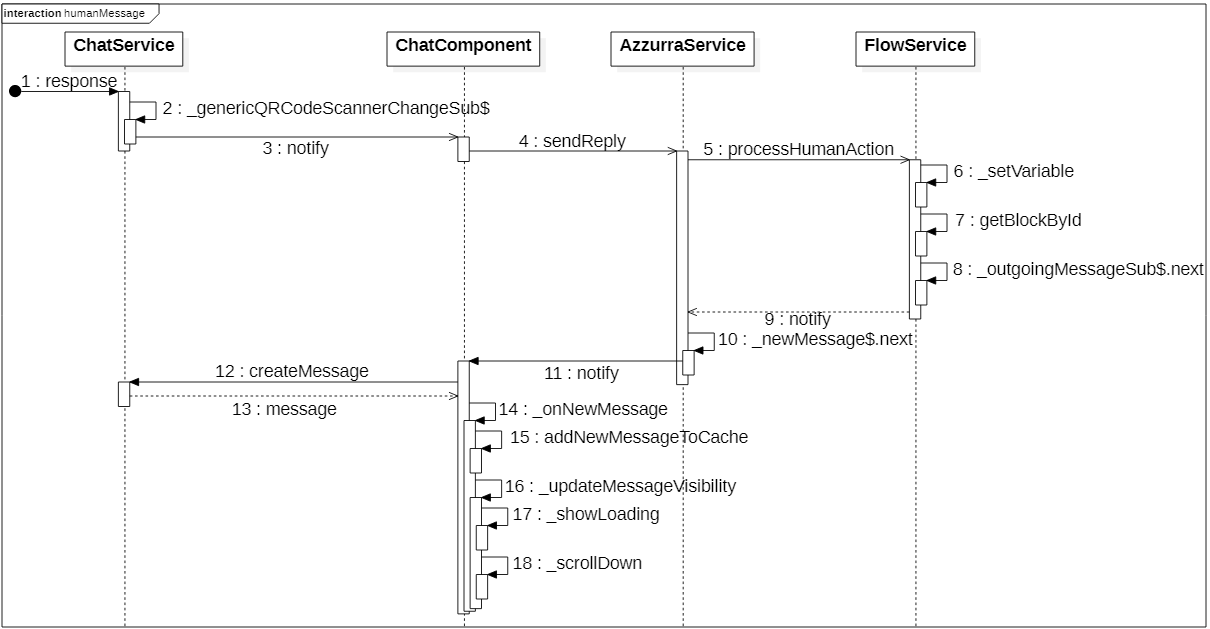
\includegraphics[height=11cm, width=13cm]{sd_human_mx.png}
	\caption{Diagramma di sequenza del processo di generazione del messaggio del bot Azzurra}\label{fig:mxHuman}
\end{figure}
\begin{enumerate}
	\item Quando l'utente esegue un'azione che genera una risposta da parte sua, il ChatService emette il valore della risposta ogni volta che un Widget la riceve;
	\item Nel ChatComponent esiste un ascoltatore per ogni evento emesso da ogni Widget. Nella Figura~\ref{fig:mxHuman} viene rappresentato il caso in cui il Widget sia di tipo QRCODE perciò, attraverso il metodo next() di Angular, viene emesso un segnale che avvisa a chi e in ascolto su  \_genericQRCodeScannerChangeSub\$ che è stato emesso un evento da QRCODE inserendo anche il valore letto dallo scanner;
	\item Viene notificato agli ascoltatori l'evento descritto al punto precedente;
	\item ChatComponent riceve la notifica e chiama il metodo sendReply() di AzzurraService dandogli in input il valore letto dallo scanner ricevuto dalla notifica solo se il messaggio è valido, se non lo è viene ignorato;	
	\item Il metodo sendReply() chiama a sua volta processHumanAction() di FlowService;
	\item In processHumanAction() viene creata la struttura del messaggio con la risposta dell'utente perciò, viene richiamato il metodo \_setVariable() in cui, viene impostato il valore della risposta ritornato dal Widget che è stato salvato nella variabile indicata nel campo var;
	\item In processHumanAction() viene richiamato il metodo getBlockId() che verifica se il Widget abbia al suo interno un proprio campo target, se sì viene impostato come prossimo blocco di conversazione il blocco che ha il codice identificativo uguale a quello contenuto nel target, se invece non ha un campo target proprio si va a prendere il valore del campo target del blocco e si imposta il suo valore come prossimo blocco da eseguire;
	\item Attraverso il metodo next() di Angular, viene emesso un segnale che avvisa a chi e in ascolto su \_outgoingMessageSub\$ che è stato emesso un nuovo messaggio;
	\item Viene notificato agli ascoltatori l'evento descritto al punto precedente;
	\item AzzurraService riceve la notifica e tramite il metodo next() avvisa e invia la struttura del nuovo messaggio a tutti coloro che sono in ascolto su \_newMessage\$;
	\item Viene notificato agli ascoltatori l'evento descritto al punto precedente;
	\item ChatComponent riceve il messaggio e chiama il metodo createMessage() di ChatService passandogli il messaggio ricevuto. Questo metodo si occuperà di far creare il messaggio grafico nel modo corretto. In questo caso il messaggio e di tipo umano perciò verrà creato secondo una certa specifica;
	\item Viene ritornato il messaggio a ChatComponent;
	\item Infine, per visualizzare il messaggio sulla \emph{chat}, vengono rifatte le stesse operazioni che erano state fatte per il messaggio del \gls{bot}\ap{[g]} Azzurra.
\end{enumerate}

             % Concept Preview
% !TEX encoding = UTF-8
% !TEX TS-program = pdflatex
% !TEX root = ../tesi.tex

%**************************************************************
\chapter{Flussi conversazionali prodotti}
\label{cap:flussi di conversazione}
%**************************************************************

\intro{In questo capitolo verrà descritto il lavoro che è stato fatto di analisi, progettazione e implementazione dei flussi conversazioniali per Azzurra creati durante lo stage.}\\

%**************************************************************
\section{Analisi dei requisiti}
\subsection{Descrizione del problema}
Durante lo stage è stato deciso, di comune accordo con il tutor aziendale, di costruire due flussi conversazionali per il \g{bot} Azzurra, nello specifico:
\begin{itemize}
	\item \textbf{DeskBooking}: Questo flusso conversazionale consiste nel gestire le prenotazioni di un posto a sedere. Deve esserci la possibilità di richiedere una nuova prenotazione, visualizzare la lista delle proprie prenotazioni e infine, scannerrizzare un \g{QR code},  messo nel posto a sedere, per controllare se il lavoratore può usufruire del posto e riscattare il posto a sedere. C'è quindi bisogno di integrare un lettore di \g{QR code} in Azzurra per poter fare il controllo, perciò, si deve poter aprire la fotocamera, scannerizzare il \g{QR code} che verrà usato e dopo il controllo, comunicare l'esito della verifica al lavoratore;
	\item \textbf{Planning}: Questo flusso conversazionale consiste nel far visualizzare al lavoratore il lavoro che deve svolgere. Deve esserci la possibilità di richiedere la visualizzazione del lavoro pianificato di uno specifico giorno oppure la possibilità di vedere il lavoro pianificato per tutta la settimana.
\end{itemize}
\subsection{Requisiti}
Ogni requisito sarà strutturato come segue:
\begin{itemize}
	\item Identificativo: \textbf{R[Importanza][Tipologia][Codice]}\\
	Dove:
	\begin{itemize}
		\item \textbf{Importanza:}
		\begin{itemize}
			\item \textbf{1}: Requisito obbligatorio, ovvero vincolante in quanto primario e fondamentale;
			\item \textbf{2}: Requisito desiderabile, ovvero non strettamente necessario ma che porta valore aggiunto riconoscibile;
			\item \textbf{3}: Requisito opzionale, ovvero relativamente utile.
		\end{itemize}
		\item \textbf{Tipologia:}
		\begin{itemize}
			\item \textbf{F}: Funzionale, definisce una funzione di un sistema di uno o più dei suoi componenti
			\item \textbf{Q}: Qualitativo, definisce un requisito per garantire la qualità per un certo aspetto del prodotto
			\item \textbf{P}: Prestazionale, definisce un requisito che garantisce efficienza prestazionale nel prodotto
			\item \textbf{V}: Vincolo, definisce un requisito volto a far rispettare un dato vincolo
		\end{itemize}
		\item \textbf{Codice:} Viene utilizzato per identificare univocamente il requisito tramite un numero progressivo\\
	\end{itemize}
\end{itemize}
Dopo un’analisi del problema sono stati individuati i seguenti requisiti
\begin{table}[h]%
	\rowcolors{2}{grigetto}{white}
		\renewcommand{\arraystretch}{1.5}
	\centering
	\begin{tabularx}{\textwidth}{c X}
		\hline	
		\rowcolor{heavenly}
		\intest{Codice} &  \intest{Descrizione} \\	
		\hline			
		R1F1 & Il lavoratore deve poter accedere alla funzionalità di "Prenotazione posto".\\
		R1F2 & Il lavoratore deve poter inserire una nuova prenotazione di un posto a sedere.\\
		R1F3 & Il lavoratore deve poter visualizzare le sue prenotazioni.\\
		R1F4 & Il lavoratore deve poter scansionare il \g{QR code} per poter usufruire del posto prenotato.\\
		R1F5 & Il lavoratore deve poter inserire la data in cui vuole prenotare il posto a sedere se disponibile.\\
		R1F6 & Il lavoratore deve poter inserire l'ora di inizio della prenotazione desiderata.\\
		R1F7 & Il lavoratore deve poter inserire l'ora in cui finisce la della prenotazione desiderata.\\
		R1F8 & Il lavoratore deve poter inserire la stanza del posto a sedere che desidera prenotare.\\
		R1F9 & Il lavoratore deve poter inserire il posto a sedere che desidera prenotare se disponibile.\\
		R1F10 & Il lavoratore deve poter visualizzare il messaggio di conferma se la prenotazione del posto a sedere è andata a buon fine.\\
		R1F11 & Il lavoratore deve poter visualizzare il messaggio d'errore se non è stato possibile inserire la nuova prenotazione.\\
		R1F12 & Il lavoratore deve poter visualizzare le sue prenotazioni del giorno corrente.\\
		R1F13 & Il lavoratore deve poter visualizzare le sue prenotazioni del giorno successivo.\\
		R1F14 & Il lavoratore deve poter visualizzare le sue prenotazioni di uno specifico giorno.\\
		R1F15 & Il lavoratore deve poter inserire la data del giorno in cui vuole vedere le prenotazioni.\\
		\hline	
	\end{tabularx} \hbox{}
	\caption{Tabella del tracciamento dei requisiti}
\end{table}%


\begin{table}[h]%
	\rowcolors{2}{grigetto}{white}
		\renewcommand{\arraystretch}{1.5}
	\centering
	\begin{tabularx}{\textwidth}{c X}
		\hline		
		\rowcolor{heavenly}
		\intest{Codice} &  \intest{Descrizione} \\	
		\hline
		R1F16 & Il lavoratore, per ogni prenotazione, deve poter visualizzare l'ora di inizio della prenotazione.\\
		R1F17 & Il lavoratore, per ogni prenotazione, deve poter visualizzare l'ora in cui finisce la prenotazione.\\		
		R1F18 & Il lavoratore, per ogni prenotazione, deve poter visualizzare la stanza della prenotazione.\\
		R1F19 & Il lavoratore, per ogni prenotazione, deve poter visualizzare il posto della prenotazione.\\	
		R1F20 & Il lavoratore, dopo avere scannerizzato il \g{QR code} del posto a sedere, deve ricevere un messaggio di conferma che lo informa che può usufruire del posto a sedere.\\
		R1F21 & Il lavoratore, dopo avere scannerizzato il \g{QR code} del posto a sedere, deve ricevere un messaggio d'errore che lo informa che non può usufruire del posto a sedere.\\
		R1F22 & Il lavoratore deve poter visualizzazione la pianificazione di uno specifico giorno.\\
		R1F23 & Il lavoratore deve poter visualizzazione la pianificazione della settimana corrente.\\
		R1F24 & Il lavoratore deve poter inserire la data del giorno in cui vuole vederne la pianificazione del lavoro a lui assegnato.\\
		R1F25 & Il lavoratore deve poter visualizzare la data del giorno del lavoro pianificato.\\
		R1F26 & Il lavoratore deve poter visualizzare l'ora d'inizio del lavoro pianificato.\\
		R1F27 & Il lavoratore deve poter visualizzare l'ora di terminazione del lavoro pianificato.\\
		R1F28 & Il lavoratore deve poter visualizzare il lavoro che è stato pianificato per essere svolto.\\
		R1V1 & Per implementare i flussi conversazionali devono essere usati Angular e Ionic.\\
		R1V2 & Per gestire la fotocamera per la lettura del \g{QR code} deve essere usato il \emph{plugin} di Cordova, QR Scanner.\\
		\hline	
	\end{tabularx} \hbox{}
	\caption{Tabella del tracciamento dei requisiti}
\end{table}%
\clearpage
\section{Progettazione}
Dopo aver individuato i requisiti che descrivono i flussi da costruire, si è passati alla progettazione dei flussi. Come spiegato nel capitolo precedente i flussi conversazionali sono un insieme di blocchi che asseconda del tipo di appartenenza svolgono determinate funzioni. Grazie a ciò, la progettazione dei due flussi è iniziata con l'inserimento dei blocchi corretti e il collegamento tra di essi, ottenendo così due diagrammi che rappresentano i due flussi dove viene mostrato che passi deve fare il \g{bot} Azzurra durante la conversazione con l'utente umano. Successivamente si sono progettati i metodi da aggiungere a quelli esistenti per poter creare i messaggi nel modo corretto.\\
Di seguito vengono illustrati i diagrammi dei flussi fatti.

\subsection{Gestione delle prenotazioni dei posti}
Nei seguenti diagrammi viene mostrato l'insieme dei blocchi che fanno parte del flusso conversazionale DeskBooking. Per comodità il flusso invece di usare un unico diagramma molto grande si è deciso di rappresentare il flusso attraverso tre diagrammi più piccoli.

\begin{figure}[h]
	\centering
	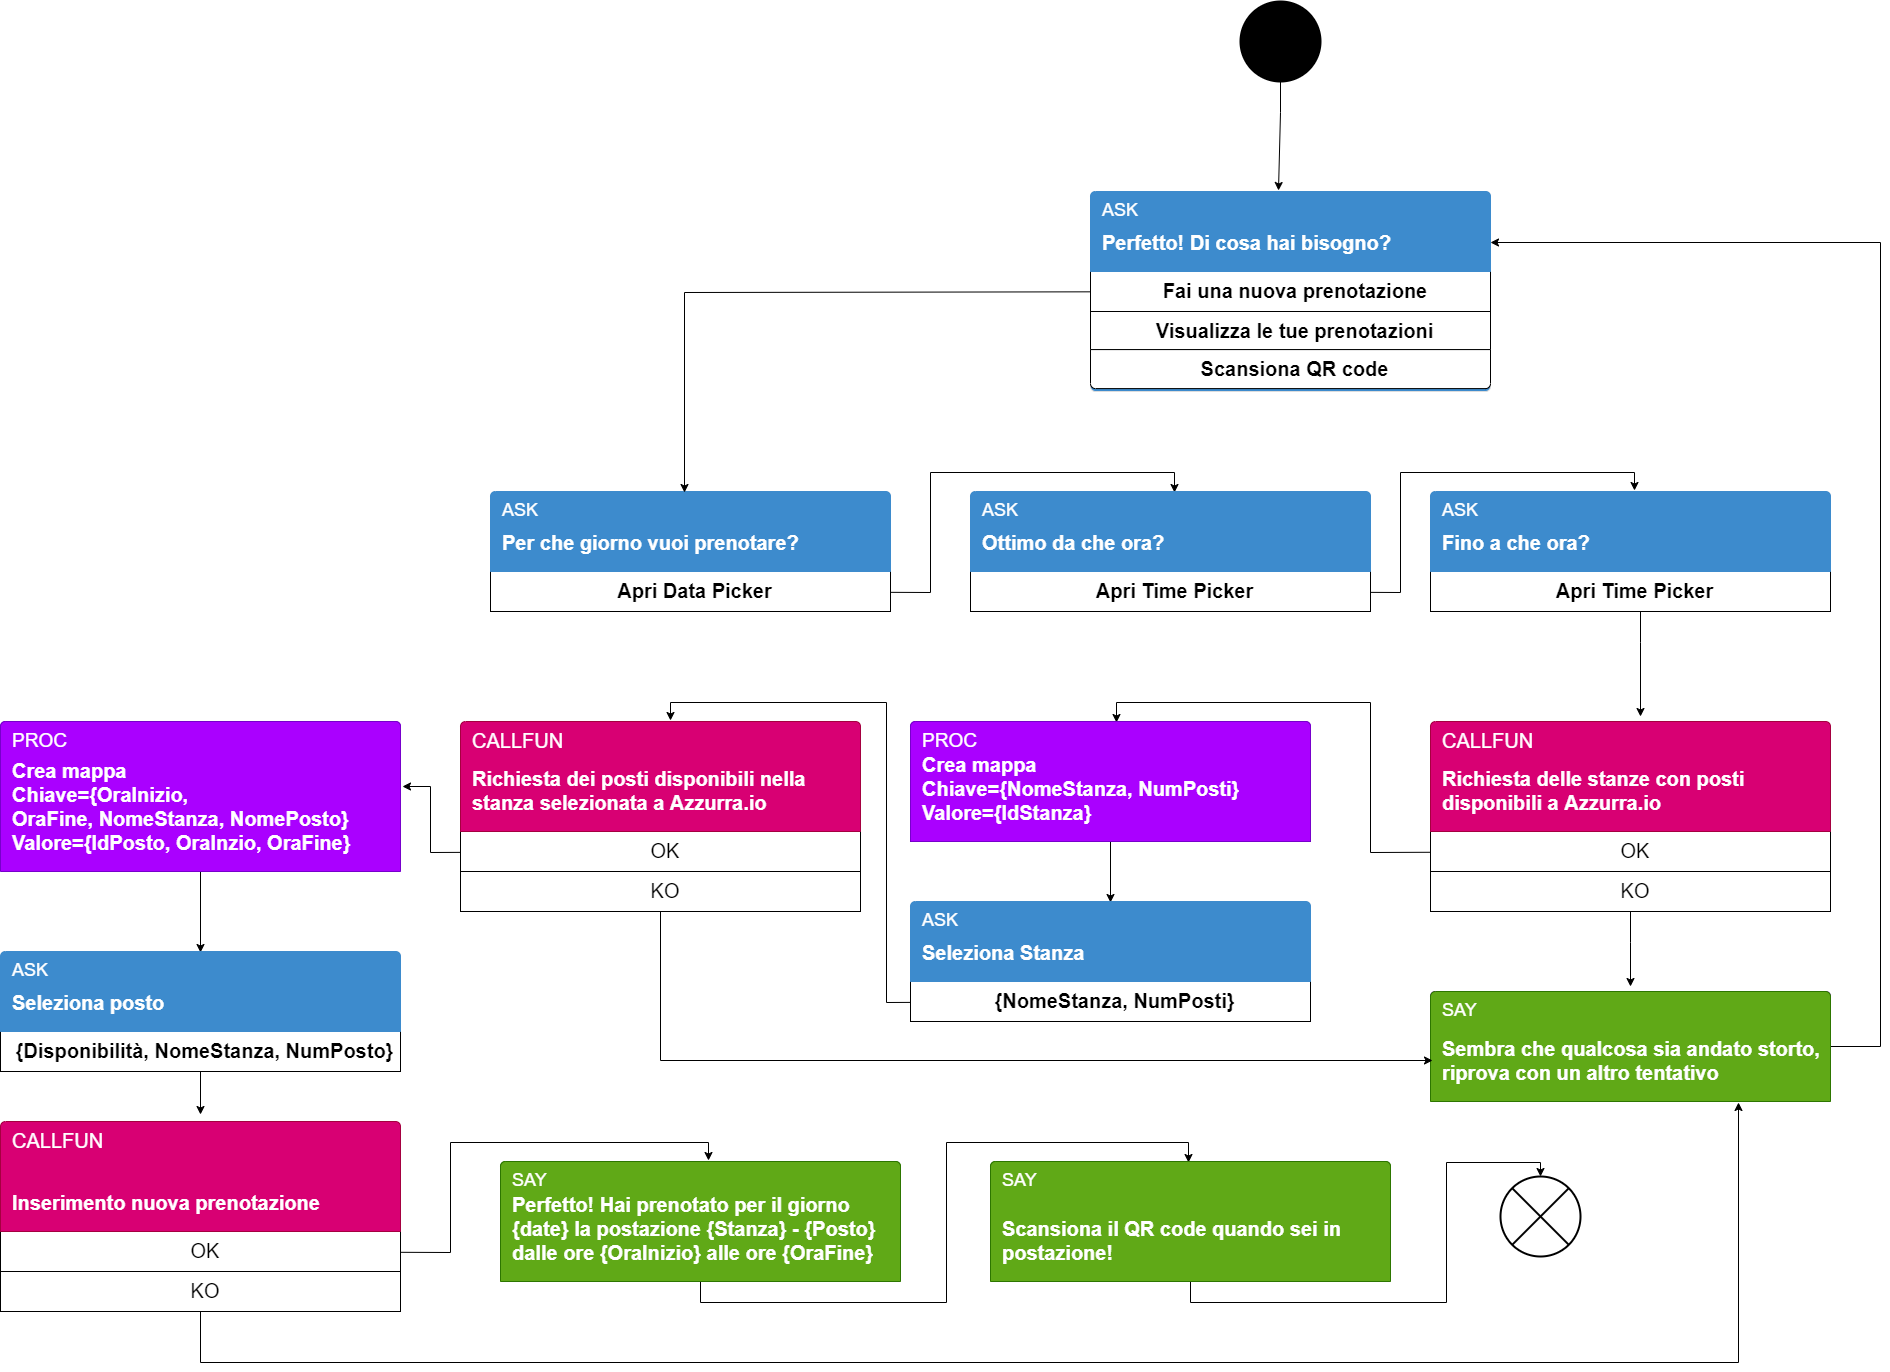
\includegraphics[scale=0.25]{chatbot/chatbot1.png}
	\caption{Diagramma per l'inserimento di una nuova prenotazione del flusso DeskBooking}\label{fig:ins}
\end{figure}

La Figura~\ref{fig:ins} rappresenta il ramo del flusso Deskbooking dedicato all'inserimento di una nuova prenotazione. È così composto:
\begin{enumerate}
	\item Il flusso inizia con un blocco ASK che chiede all'utente se vuole inserire una nuova prenotazione o scansionare un \g{QR code};
	\item Nel caso in cui l'utente voglia inserire una nuova prenotazione, attraverso un blocco ASK viene chiesta la data che vuole inserire per la prenotazione. Viene progettato che l'inserimento della data viene fatta attraverso il DATEPICKER;
	\item Successivamente tramite un blocco ASK viene chiesta l'ora di inizio per la prenotazione. L'inserimento dell'ora avviene tramite il TIMEPICKER;
	\item Viene rifatta la stessa operazione del punto precedente ma chiedendo la data in cui finisce la prenotazione;
	\item Terminato il punto precedente, l'utente ha inserito l'intervallo di tempo all'interno del quale desidera effettuare una prenotazione di un posto a sedere. Attraverso il blocco CALLFUN viene chiesto a Azzurra.io quali stanze con posti liberi sono disponibili per la data e l'intervallo inseriti dall'utente;
	\item Se non ci sono stanze con posti liberi o l'operazione di richiesta va in errore, attraverso un blocco SAY viene informato l'utente della situazione e ricomincia l'esecuzione dall'inizio del flusso;
	\item Se invece ci sono stanze con posti liberi, attraverso il blocco PROC vengono formattati i dati ricevuti in modo da poterli mostrare in una forma adatta alla situazione. In questo caso viene chiesto di creare una mappa con chiave contenente il nome della stanza e il numero dei posti, mentre come valore l'identificativo della stanza. Quando si vorrà mostrare questi dati, verrà solo mostrato la chiave dei dati;
	\item Tramite il blocco ASK vengono mostrate le stanze disponibili mostrando i dati secondo la formattazione fatta al punto precedente;
	\item L'utente sceglie la stanza è viene controllato se nel frattempo è ancora disponibile e chiede quali posti a sedere sono liberi;
	\item Se avviene un errore di connessione o non ci sono più posti liberi si torna al punto 6 spiegato precedentemente;
	\item I dati ricevuti vengono formattati attraverso il blocco PROC creando la mappa con chiave contenente ora di inizio, orario di terminazione, nome stanza e nome posto a sedere, mentre come valore conterrà l'identificativo del posto a sedere, l'orario di inizio e di fine;
	\item Viene chiesto all'utente, attraverso un blocco ASK, di scegliere uno dei posti a sedere liberi;
	\item Viene contattato Azzurra.io con il blocco CALLFUN per inserire la nuova prenotazione;
	\item Se avviene un errore nell'inserimento viene eseguito il punto 6;
	\item Se l'operazione va a buon fine viene comunicato all'utente l'esito positivo dell'operazione, ricordandogli i dati della prenotazione e di scansionare il \g{QR code} per riscattare il posto a sedere. Il flusso poi termina.
\end{enumerate}

\begin{figure}[h]
	\centering
	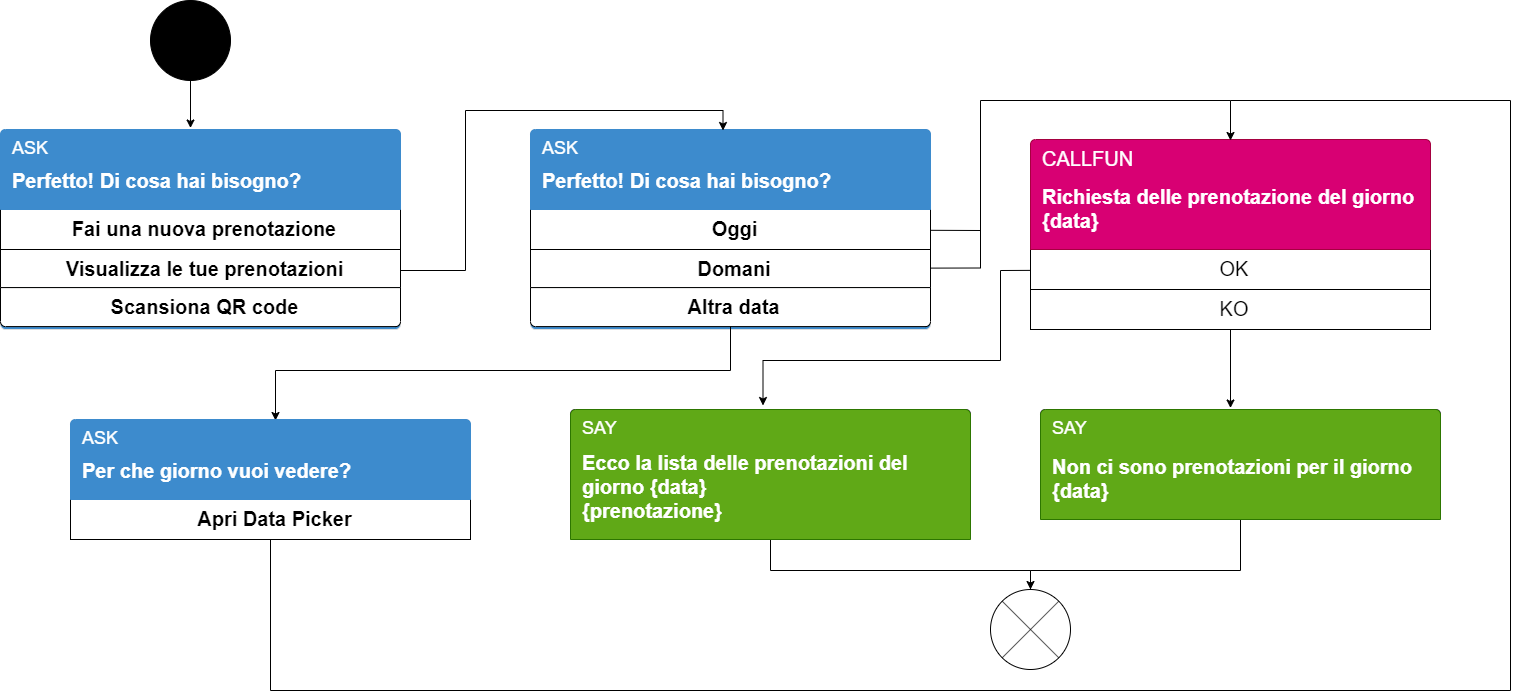
\includegraphics[scale=0.27]{chatbot/chatbot2.png}
	\caption{Diagramma per la visualizzazione delle prenotazioni del flusso DeskBooking}\label{fig:vis}
\end{figure}

La Figura~\ref{fig:vis} rappresenta il ramo del flusso Deskbooking dedicato alla visualizzazione delle prenotazioni. È così composto:
\begin{enumerate}
	\item Il flusso inizia con un blocco ASK che chiede all'utente se vuole inserire una nuova prenotazione o scansionare un \g{QR code};
	\item Nel caso in cui l'utente voglia visualizzare le sue prenotazione, viene chiesto attraverso un blocco ASK se vuole sapere le prenotazione del giorno corrente o del giorno successivo o di un altro giorno;
	\item Nel caso l'utente voglia vedere le sue prenotazioni del giorno corrente o del giorno successivo verrà fatta una richiesta a Azzurra.io per ottenere le prenotazioni della data inserita dall'utente. La richiesta viene fatta attraverso il blocco CALLFUN;
	\item Se invece l'utente vuole vedere le sue prenotazioni di una data diversa dal giorno corrente o successivo, attraverso un blocco ASK viene chiesta la data che vuole inserire per la visualizzazione. L'inserimento della data viene fatta attraverso il DATEPICKER, successivamente si esegue il punto 3 per la richiesta;
	\item Se ci sono prenotazioni queste vengono mostrate all'utente, se invece avviene un errore o non ci sono prenotazioni fatte da lui, verrà avvisato di tale evento. Dopo questo passo il flusso termina\\
\end{enumerate}

\begin{figure}[h]
	\centering
	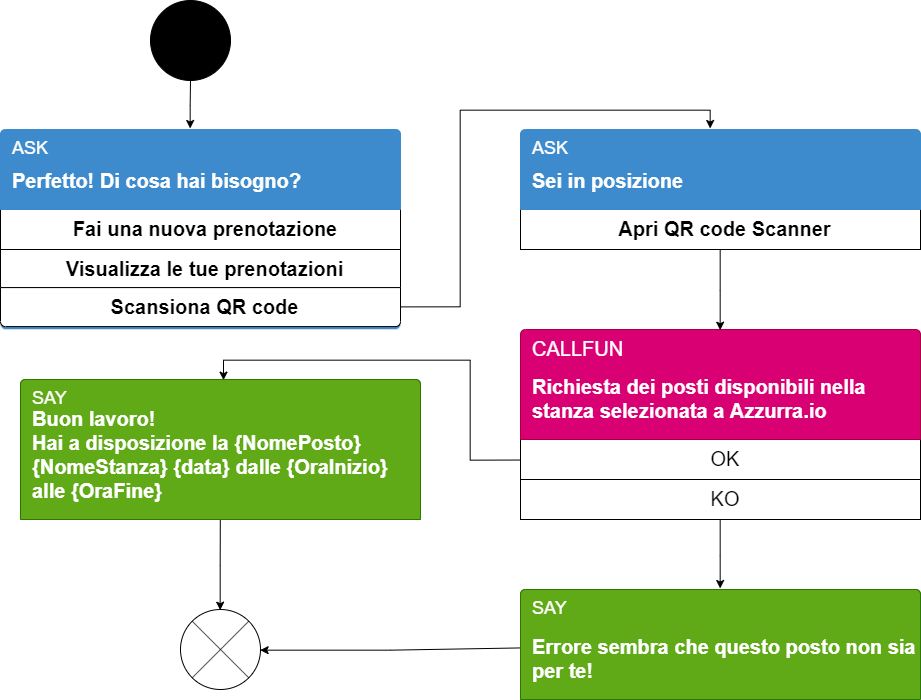
\includegraphics[scale=0.275]{chatbot/chatbot3.png}
	\caption{Diagramma per lo scansionamento del \g{QR code} del flusso DeskBooking}\label{fig:qrcode}
\end{figure}

La Figura~\ref{fig:qrcode} rappresenta il ramo del flusso Deskbooking dedicato allo scansionamento del \g{QR code}. È così composto:

\begin{enumerate}
	\item Il flusso inizia con un blocco ASK che chiede all'utente se vuole inserire una nuova prenotazione o scansionare un \g{QR code};
	\item Nel caso in cui l'utente voglia scansionare un \g{QR code} per riscattare il suo posto a sedere prenotato, viene chiesto attraverso un blocco ASK di aprire il scannerizzatore di \g{QR code}. Viene usato QRSCANNER per leggere il \g{QR code};
	\item Viene chiesto a Azzurra.io attraverso il blocco CALLFUN, se il posto a sedere può essere usato dall'utente;
	\item Se l'esito è positivo, viene comunicato all'utente che può usufruire del posto fino al termine della prenotazione. Termina così il flusso;
	\item Se l'esito è negativo, viene informato l'utente che non può usare il posto a sedere in quel momento. Termina così il flusso;
\end{enumerate}

\subsection{Visualizzazione della pianificazione}
Nel seguente diagramma viene mostrato l'insieme dei blocchi che fanno parte del flusso conversazionale Planning.

\begin{figure}[h]
	\centering
	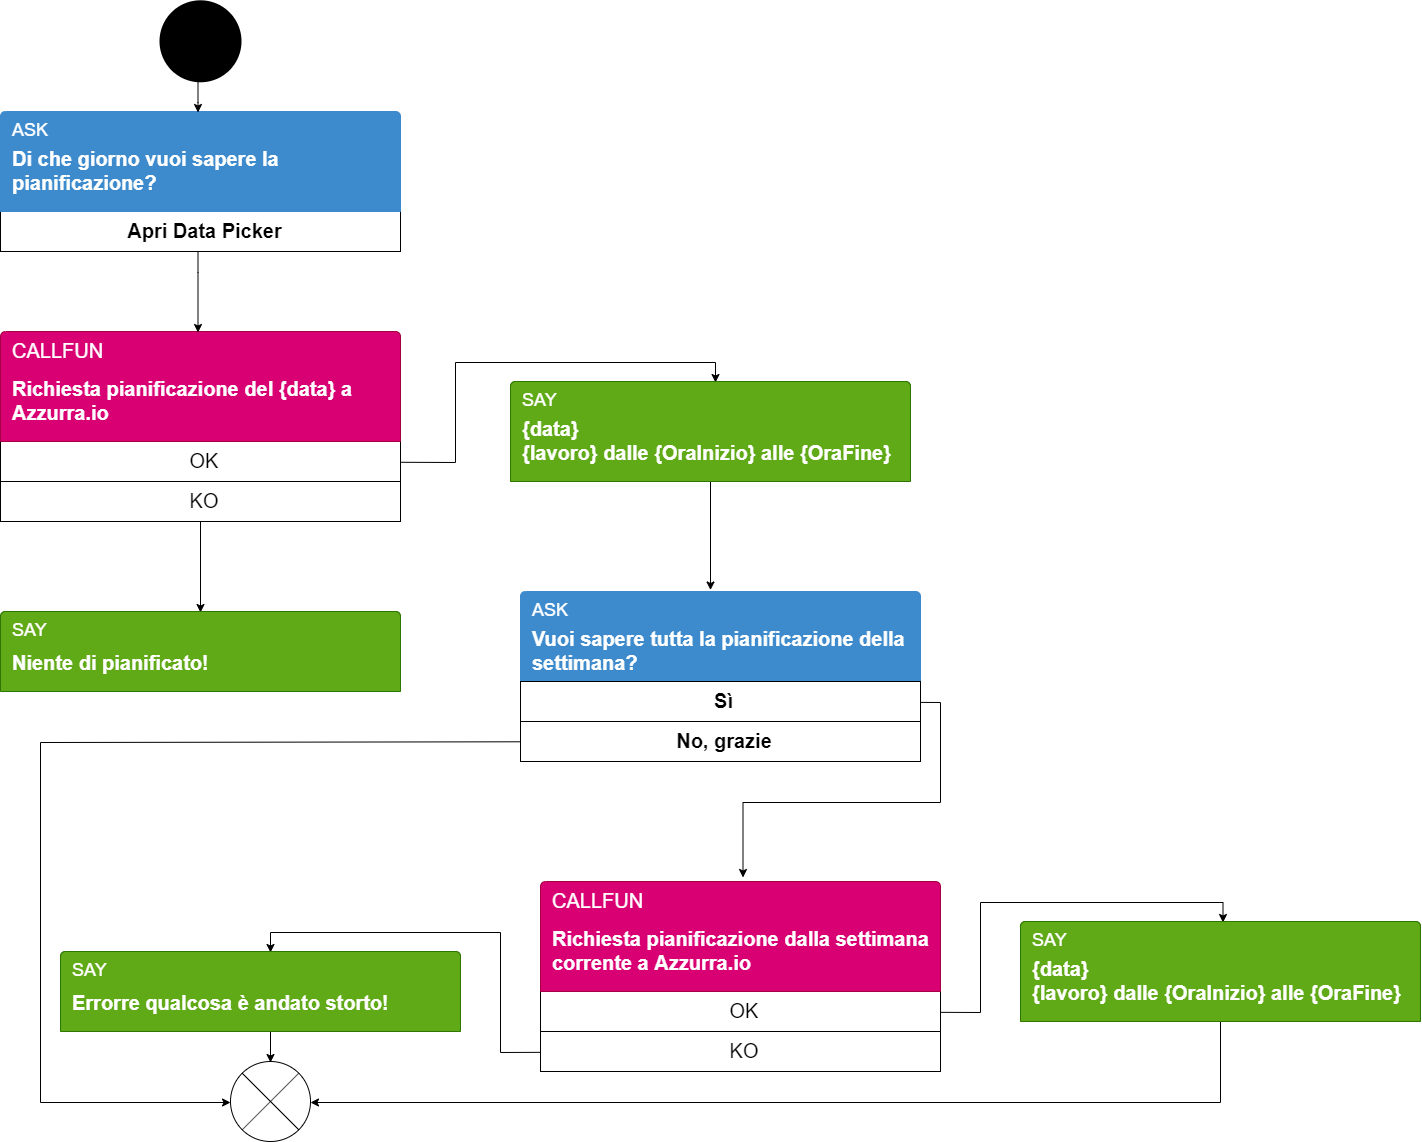
\includegraphics[scale=0.29]{chatbot/chatbot4.png}
	\caption{Diagramma per la visualizzazione della pianificazione del flusso Planning}\label{fig:plan}
\end{figure}

La Figura~\ref{fig:plan} rappresenta il ramo del flusso Planning dedicato alla visione della pianificazione del lavoro da svolgere.
\begin{enumerate}
	\item Il flusso inizia con un blocco ASK che chiede all'utente di quale giorno vuole vedere la pianificazione. L'inserimento della data viene fatta attraverso il DATEPICKER;
	\item Viene fatta richiesta a Azzurra.io, utilizzando il blocco CALLFUN, di trovare la pianificazione del giorno indicato dall'utente;
	\item Se non viene trovato nulla allora l'utente viene avvisato tramite un blocco SAY che non c'è niente di pianificato e il flusso termina;
	\item Se invece c'è una pianificazione disponibile per il giorno indicato dall'utente, viene visualizzata attraverso un blocco SAY;
	\item Dopo il punto precedentemente descritto viene chiesto con un blocco SAY se si vuole sapere la pianificazione di tutta la settimana;
	\item Se l'utente risponde no il flusso termina;
	\item Se l'utente risponde sì viene fatta richiesta a Azzurra.io, utilizzando il blocco CALLFUN, di trovare la pianificazione della settimana corrente;
	\item Se la richiesta va buon fine viene mostrata la pianificazione della settimana, altrimenti viene mostrato un messaggio. In entrambi i casi il flusso poi termina.
\end{enumerate}
\clearpage

\section{Codifica}
Per implementare i due flussi si sono utilizzati i \g{framework} Angular e Ionic. Grazie a Angular si è potuto strutturare un’applicazione web come una gerarchia di componenti quindi, attraverso il linguaggio TypeScript si è gestita l'\emph{application logic} mentre con \gls{HTML} e \gls{CSS} si è gestita la \emph{presentation logic}. Purtroppo solo l'uso di Angular non basta per poter sviluppare un'applicazione \emph{mobile} e non web, si è quindi usato Cordova, un \g{framework} che permette di sviluppare un'applicazione \emph{mobile} multi-piattaforma, quindi sia per \g{Android} e sia per \g{iOS}, con tecnologie web e inoltre, offre \g{api} per accedere alle funzionalità native del dispositivo, ad'esempio la fotocamera. Infatti, Cordova incapsula l'applicazione web e la esegue localmente all’interno di un’\g{applicazione nativa} che può interagire con le funzionalità del dispositivo. Per sfruttare le funzionalità di Angular e di Cordova assieme, è stato usato il \g{framework} Ionic che permette di creare un ambiente integrato che semplifica lo sviluppo di applicazioni offrendo inoltre, componenti grafiche ottimizzate per i dispositivi \emph{mobile}.\\

Per quanto riguarda la codifica, per prima cosa si è implementato una configurazione \g{JSON} per ogni flusso, dove si sono codificati i vari blocchi progettati, utilizzando la sintassi spiegata nel precedente capitolo. Una volta scritte le due configurazioni si è dovuto aggiornare il \emph{main flow} aggiungendo nel primo blocco che viene eseguito, cioè un blocco ASK dove viene chiesto che funzionalità si vuole eseguire, due BlockItem per indicare le due nuove funzionalità offerte dai due flussi prodotti. Oltre alle due nuove scelte, nel \emph{main flow} sono stati aggiunti due blocchi JUMP per permettere di mandare in esecuzione i due nuovi flussi quando l'utente ne richiede l'esecuzione, subito dopo la selezione della funzionalità desiderata da parte dell'utente.\\

Per poter creare i tre Widget, DATEPICKER, TIMEPICKER e QRSCANNER, nel createActions() ho aggiunto tre metodi per ognuno dei tre Widget, che vengono chiamati da createActions() in base al tipo di Widget da creare. In questi tre nuovi metodi viene impostato il testo che devono mostrare e nel caso dei DATEPICKER, TIMEPICKER viene impostato anche il formato del giorno e dell'ora. Per ognuno di questi metodi ho creato un metodo specifico per ogni Widget che si occupa della creazione e dell'apertura, in particolare per il metodo che crea il QRSCANNER, \_openQRcode(), viene utilizzato il ModalController di Ionic per creare la classe dove è definita l'interfaccia grafica e i metodi per il funzionamento di QRSCANNER. Il ModalController di Ionic permette di aprire una nuova finestra sopra a quella corrente per visualizza la componente Ionic definita nella nuova finestra, in questo caso la classe che implementa il lettore di \g{QR code}. Una volta finito di usare la nuova finestra essa viene chiusa si ritorna alla finestra precedente che sarà nello stato in cui era prima dell'apertura della nuova finestra. Ho dovuto perciò, implementare la classe che gestisce il lettore \g{QR code}, denominata CameraComponent, dove al suo interno richiama il \emph{plugin} di Cordova, QR Scanner. QR Scanner è un \g{api} che permette di accedere alla fotocamera del dispositivo e di scansionare i \g{QR code}. Vengono perciò definiti due metodi in CameraComponent, un metodo per l'apertura della fotocamera e la lettura del \g{QR code} e per la chiusura della fotocamera che dopo la chiusura, invia l'eventuale valore letto al ModalController. Nel CameraComponent viene definito anche il suo aspetto grafico mostrato nella Figura~\ref{fig:qrc}.\\
 
  Nel ChatComponent ho implementato il metodo \_initGenericQRCode() il quale aspetta di ricevere il valore letto dal lettore di \g{QR code}, che una volta che lo riceve, richiama il metodo sendReply() di AzzurraService per dare inizio al il processo di creazione del messaggio dell'utente umano spiegato nel capitolo precedente. \\
  
  Per quanto riguarda i metodi per il DATEPICKER e per il TIMEPICKER, essi sono molto simili a quelli per gestire il lettore \g{QR code}, l'unica differenza è che i metodi analoghi a \_openQRcode() quindi \_openDatePicker() e \_openTimePicker(), non utilizzano il ModalComponent ma viene utilizzato l'ion-datetime, una componente grafica offerto da Ionic che può essere configurato per chiedere una data oppure un intervallo temporale, il risultato viene mostrato nella Figura~\ref{fig:date} e nella Figura~\ref{fig:time}. Quindi in questi due metodi ho definito come si devono presentare i due \emph{picker} e quindi non c'è stato nemmeno bisogno di un \emph{component} apposito che li gestisca come per il QRSCANNER. 
\section{Risultati}

Nella Figura~\ref{fig:planning} viene mostrata la \emph{chat} tra Azzurra e l'utente per la visualizzazione della pianificazione, sia per un singolo giorno (prima figura) sia per tutta la settimana (seconda figura).\\

\begin{figure}[h]
	\begin{center}
		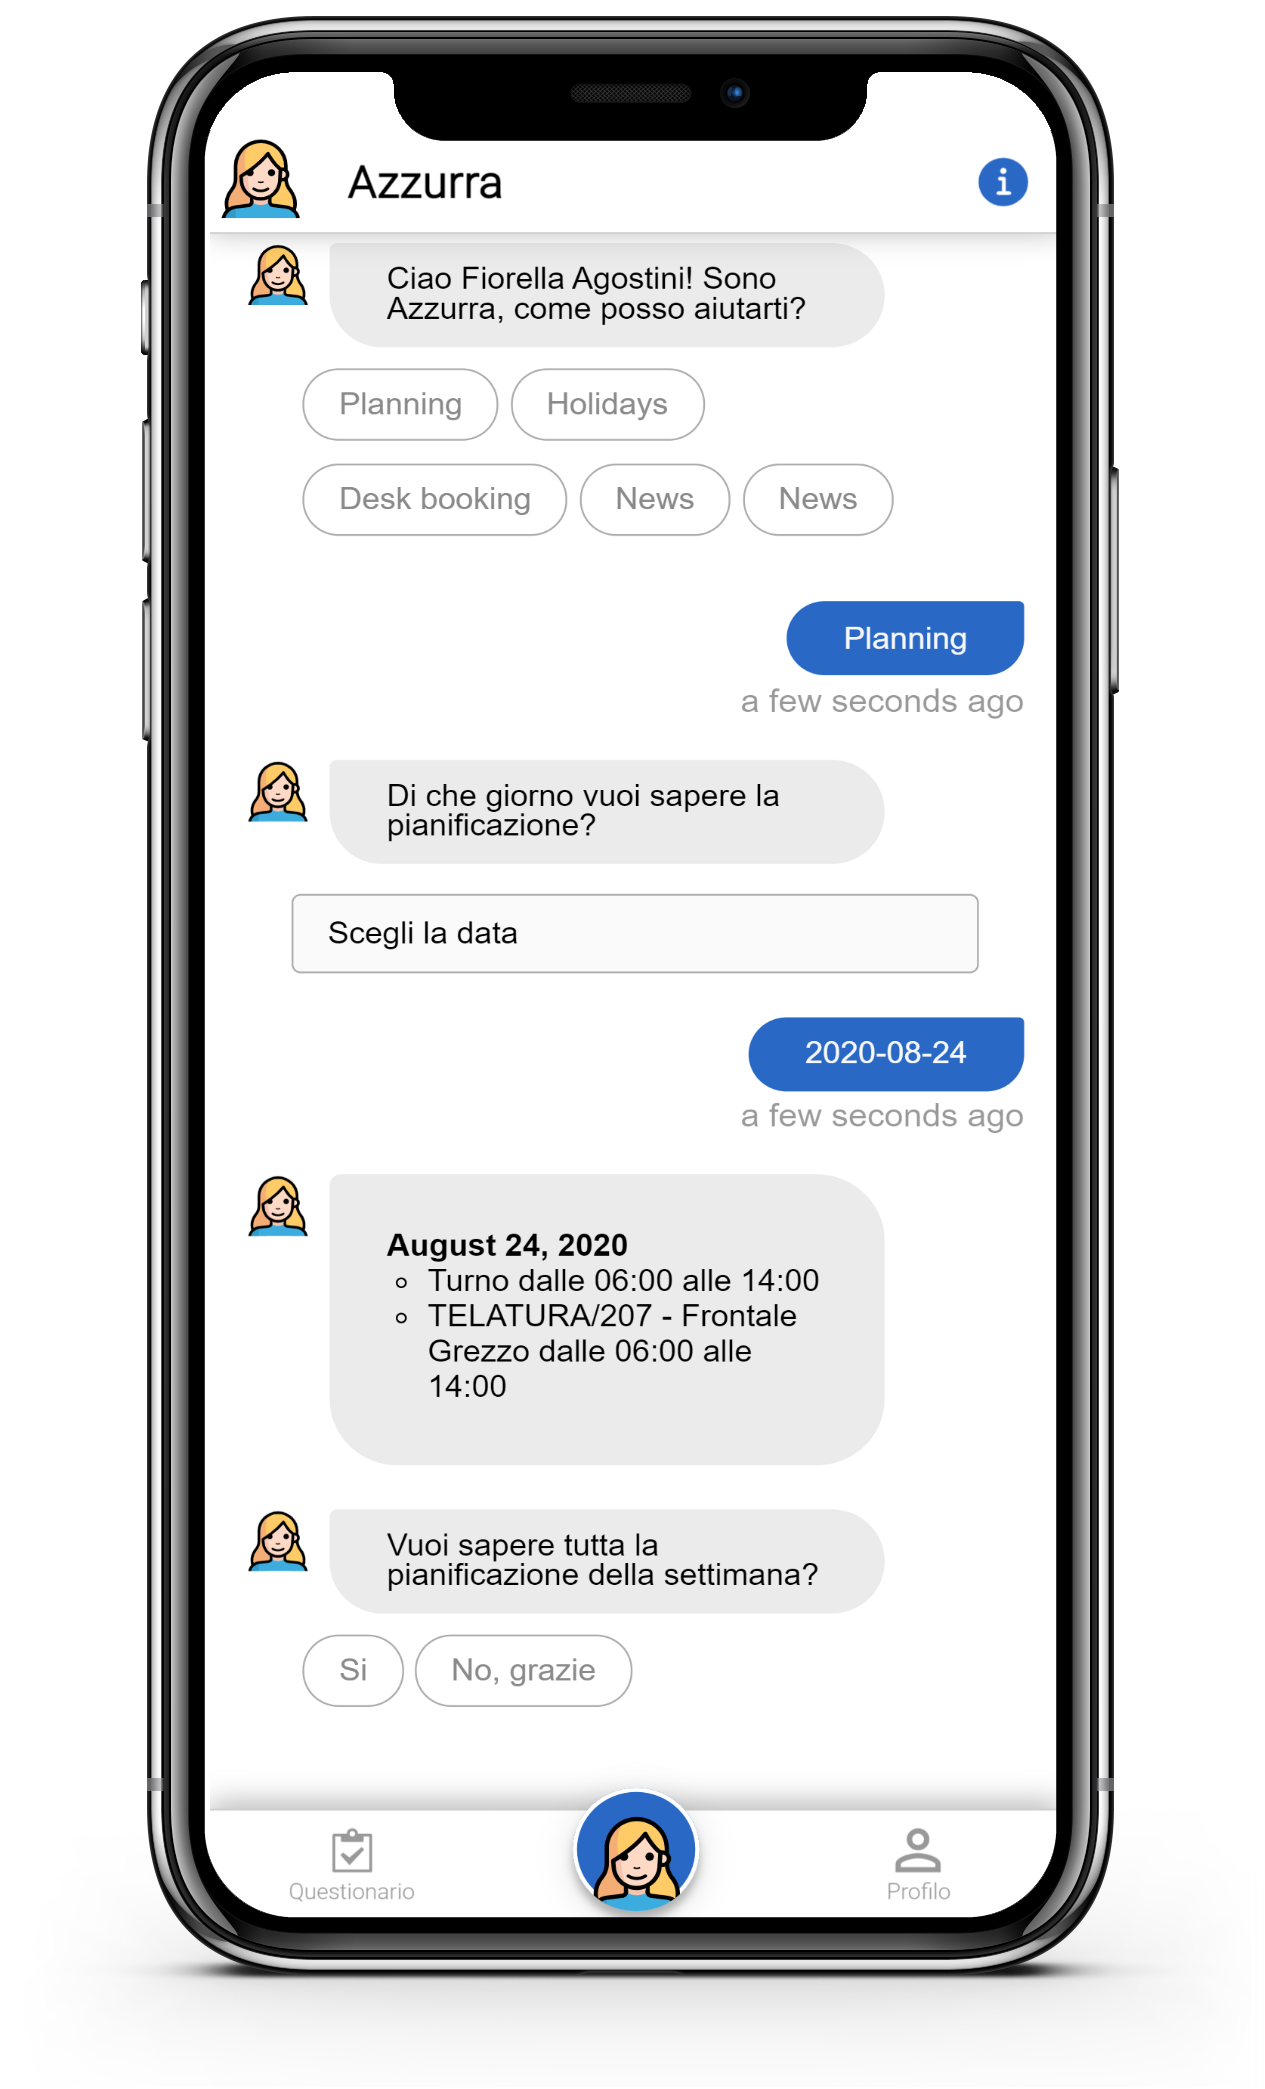
\includegraphics[scale=0.17]{day.png}\hfil
		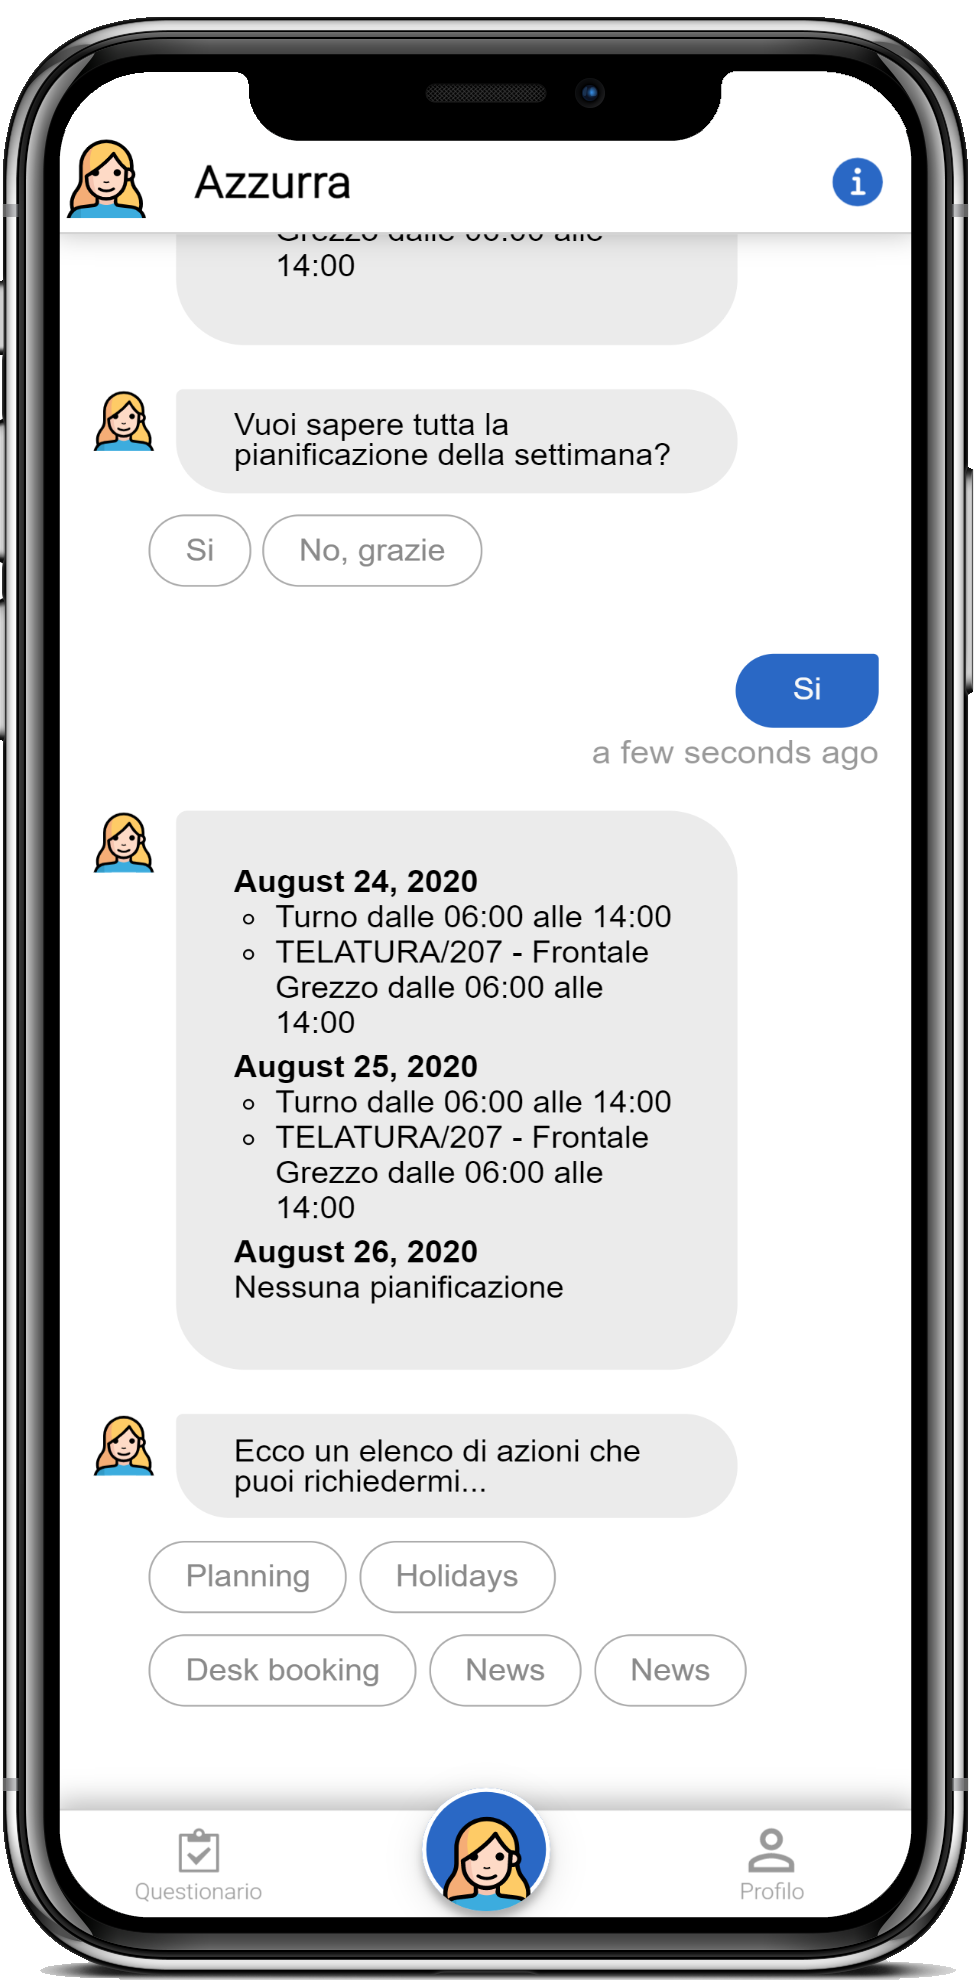
\includegraphics[scale=0.17]{week.png}
		\caption{Richiesta di visualizzazione della pianificazione}\label{fig:planning}
	\end{center}
\end{figure}

Nella Figura~\ref{fig:QRc} viene mostrata la \emph{chat} tra Azzurra e l'utente per la richiesta di visualizzazione del prenotazione dell'utente (prima figura) e la richiesta di scannerizzare il \g{QR code} per usufruire del posto prenotato (seconda figura).\\

\begin{figure}[h]
	\begin{center}
		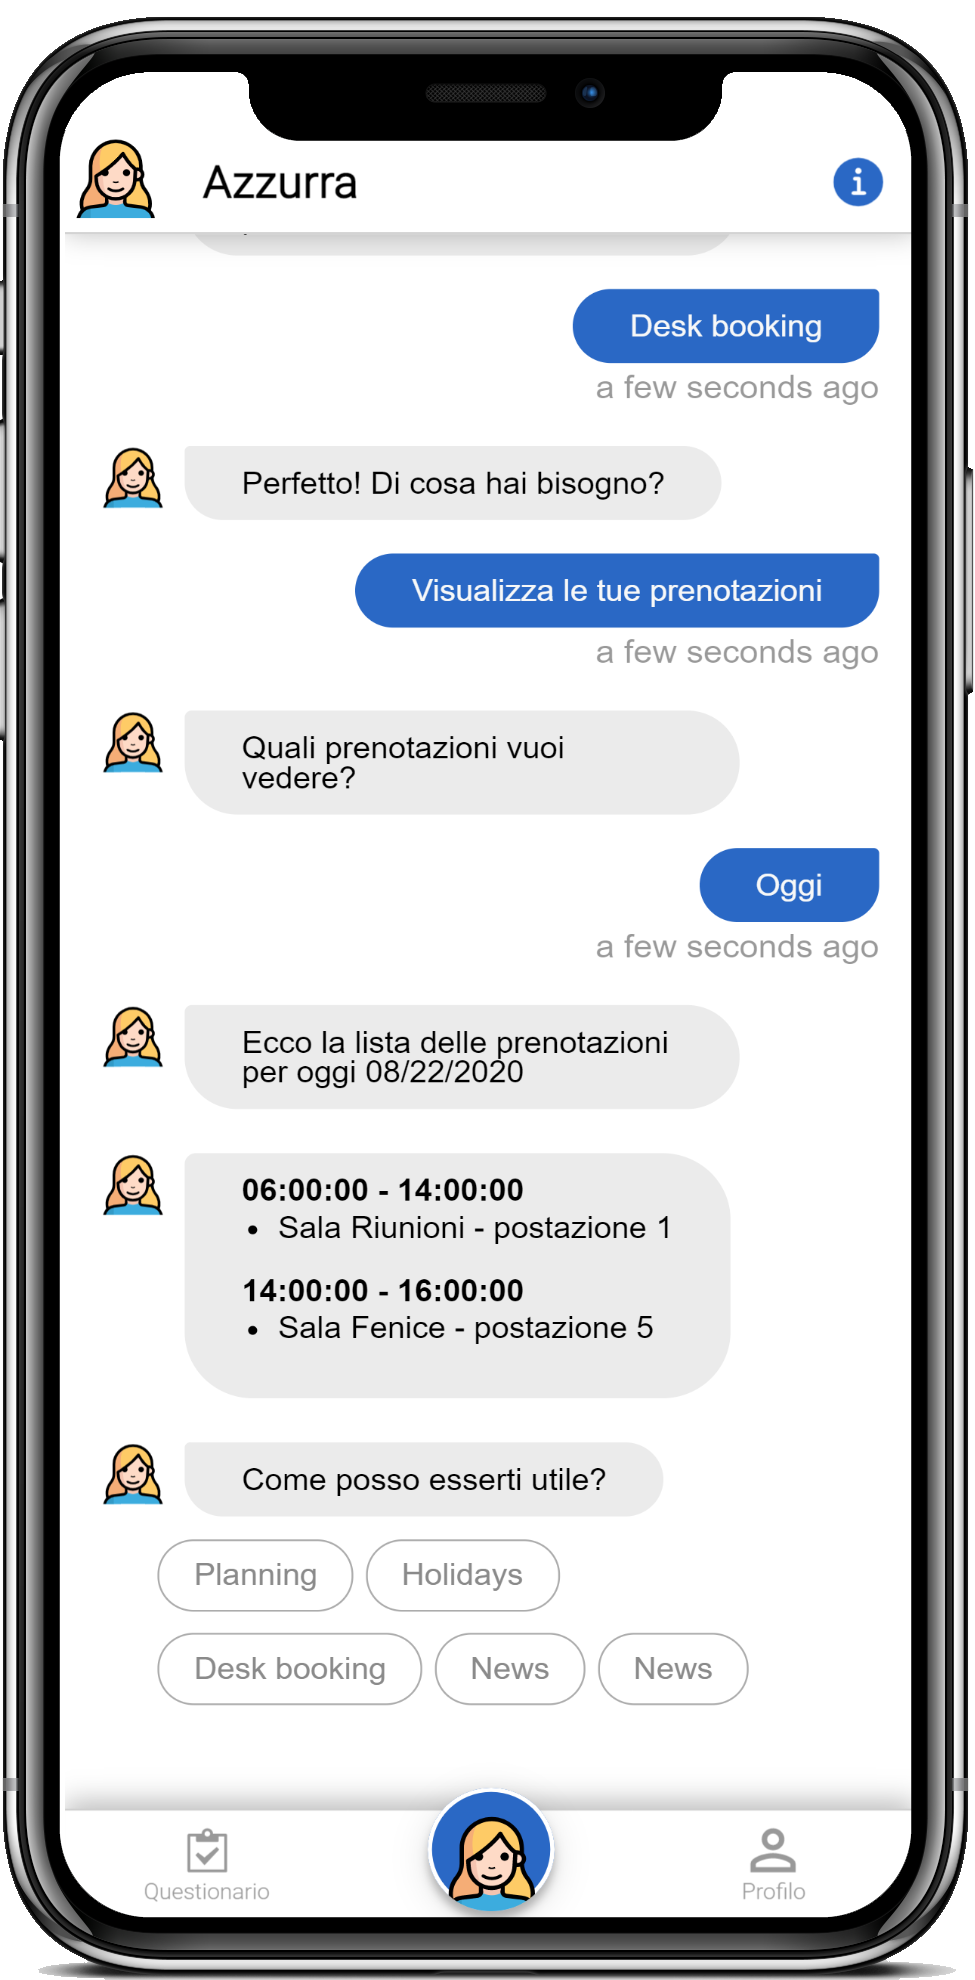
\includegraphics[scale=0.17]{visDB.png}\hfil
		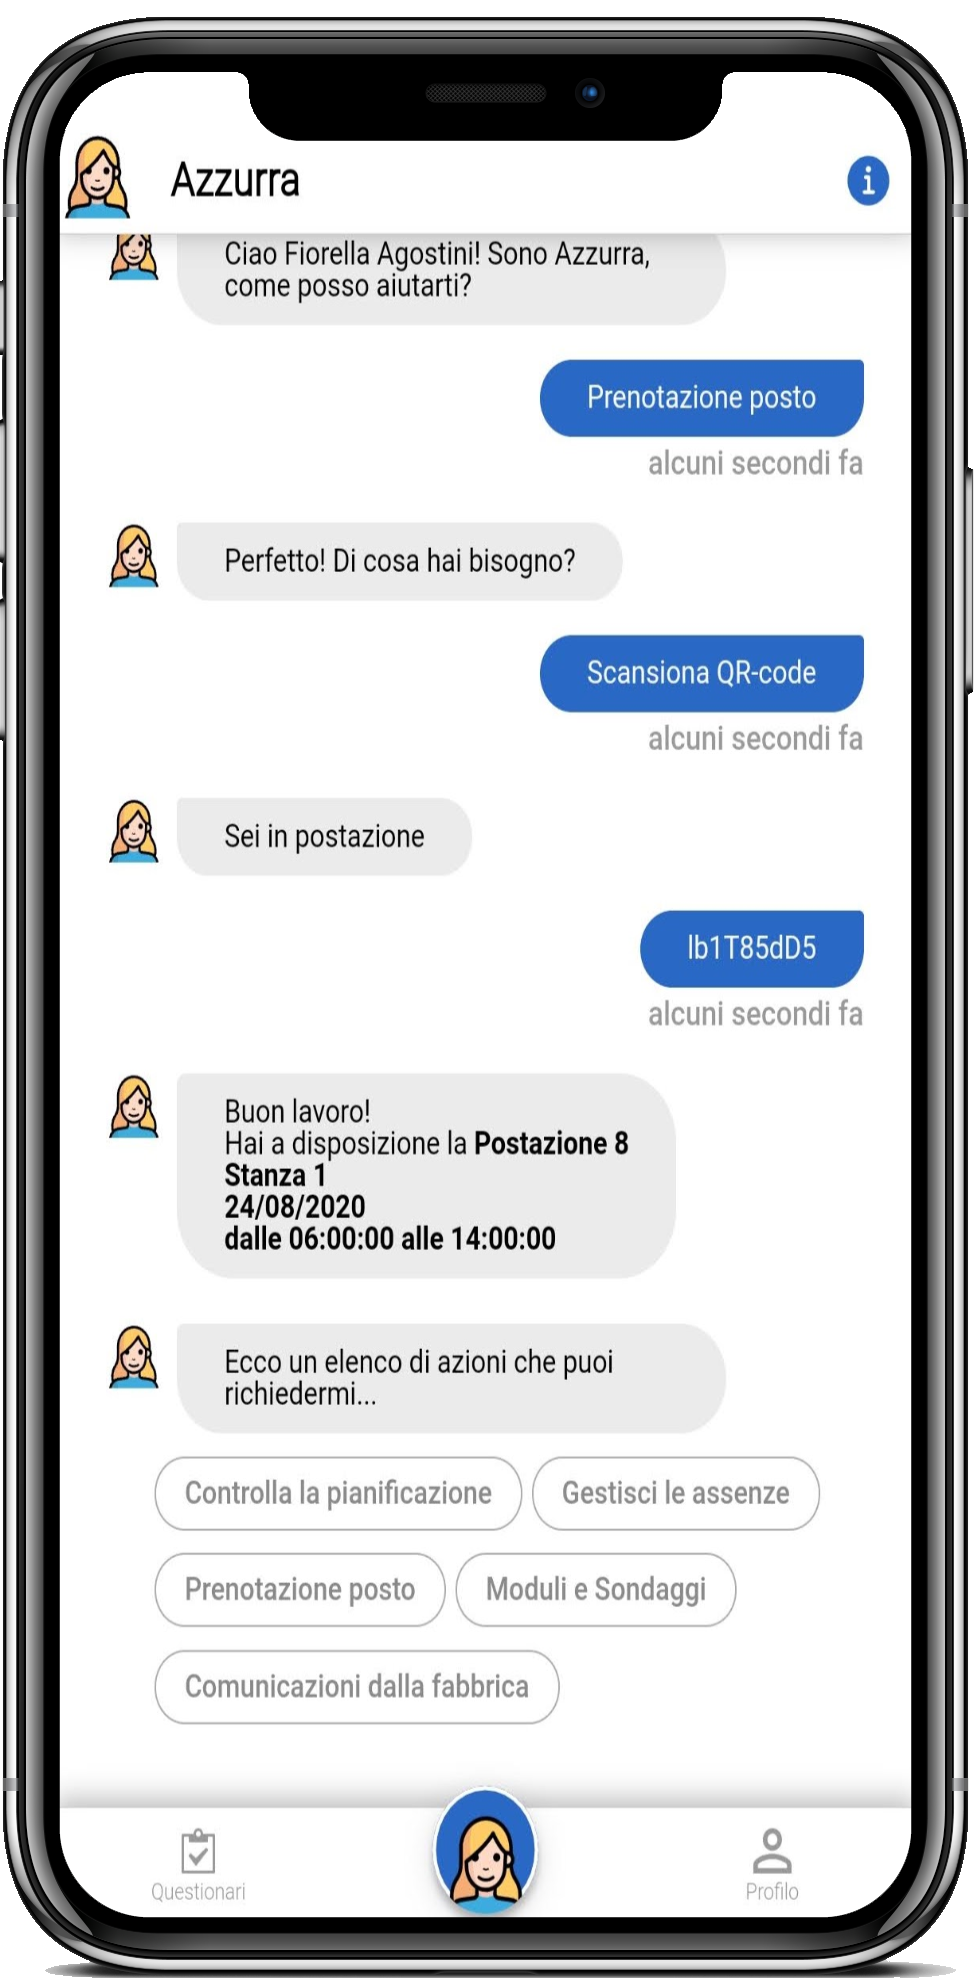
\includegraphics[scale=0.17]{qrc.png}
		\caption{Richiesta di visualizzazione delle prenotazioni e scannerizzazione di un QR code}\label{fig:QRc}
	\end{center}
\end{figure}

\begin{figure}[h]
	\begin{center}
		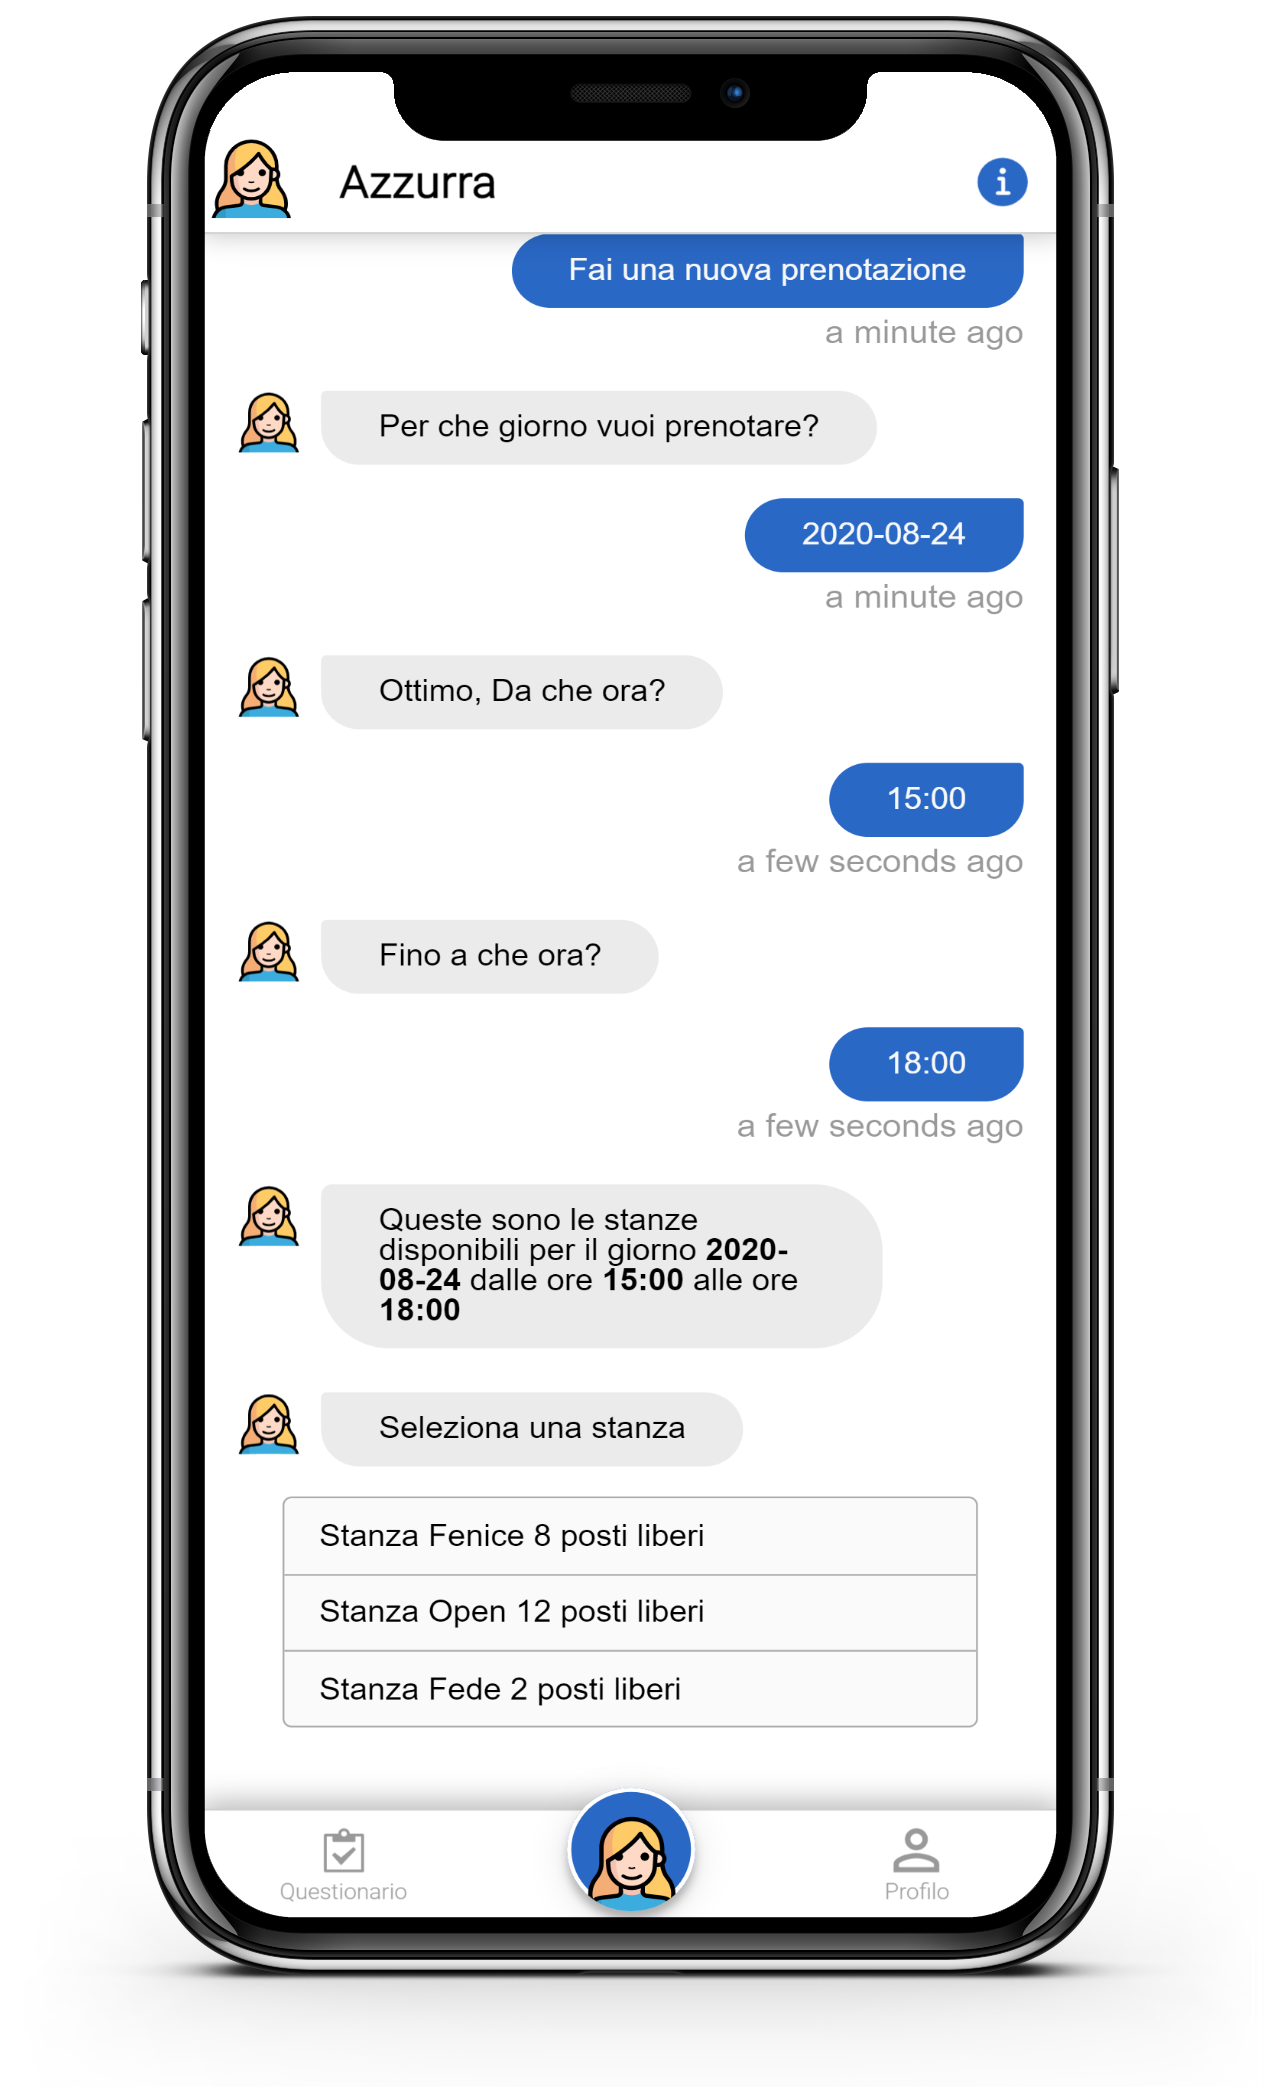
\includegraphics[scale=0.167]{DB1.png}\hfill
		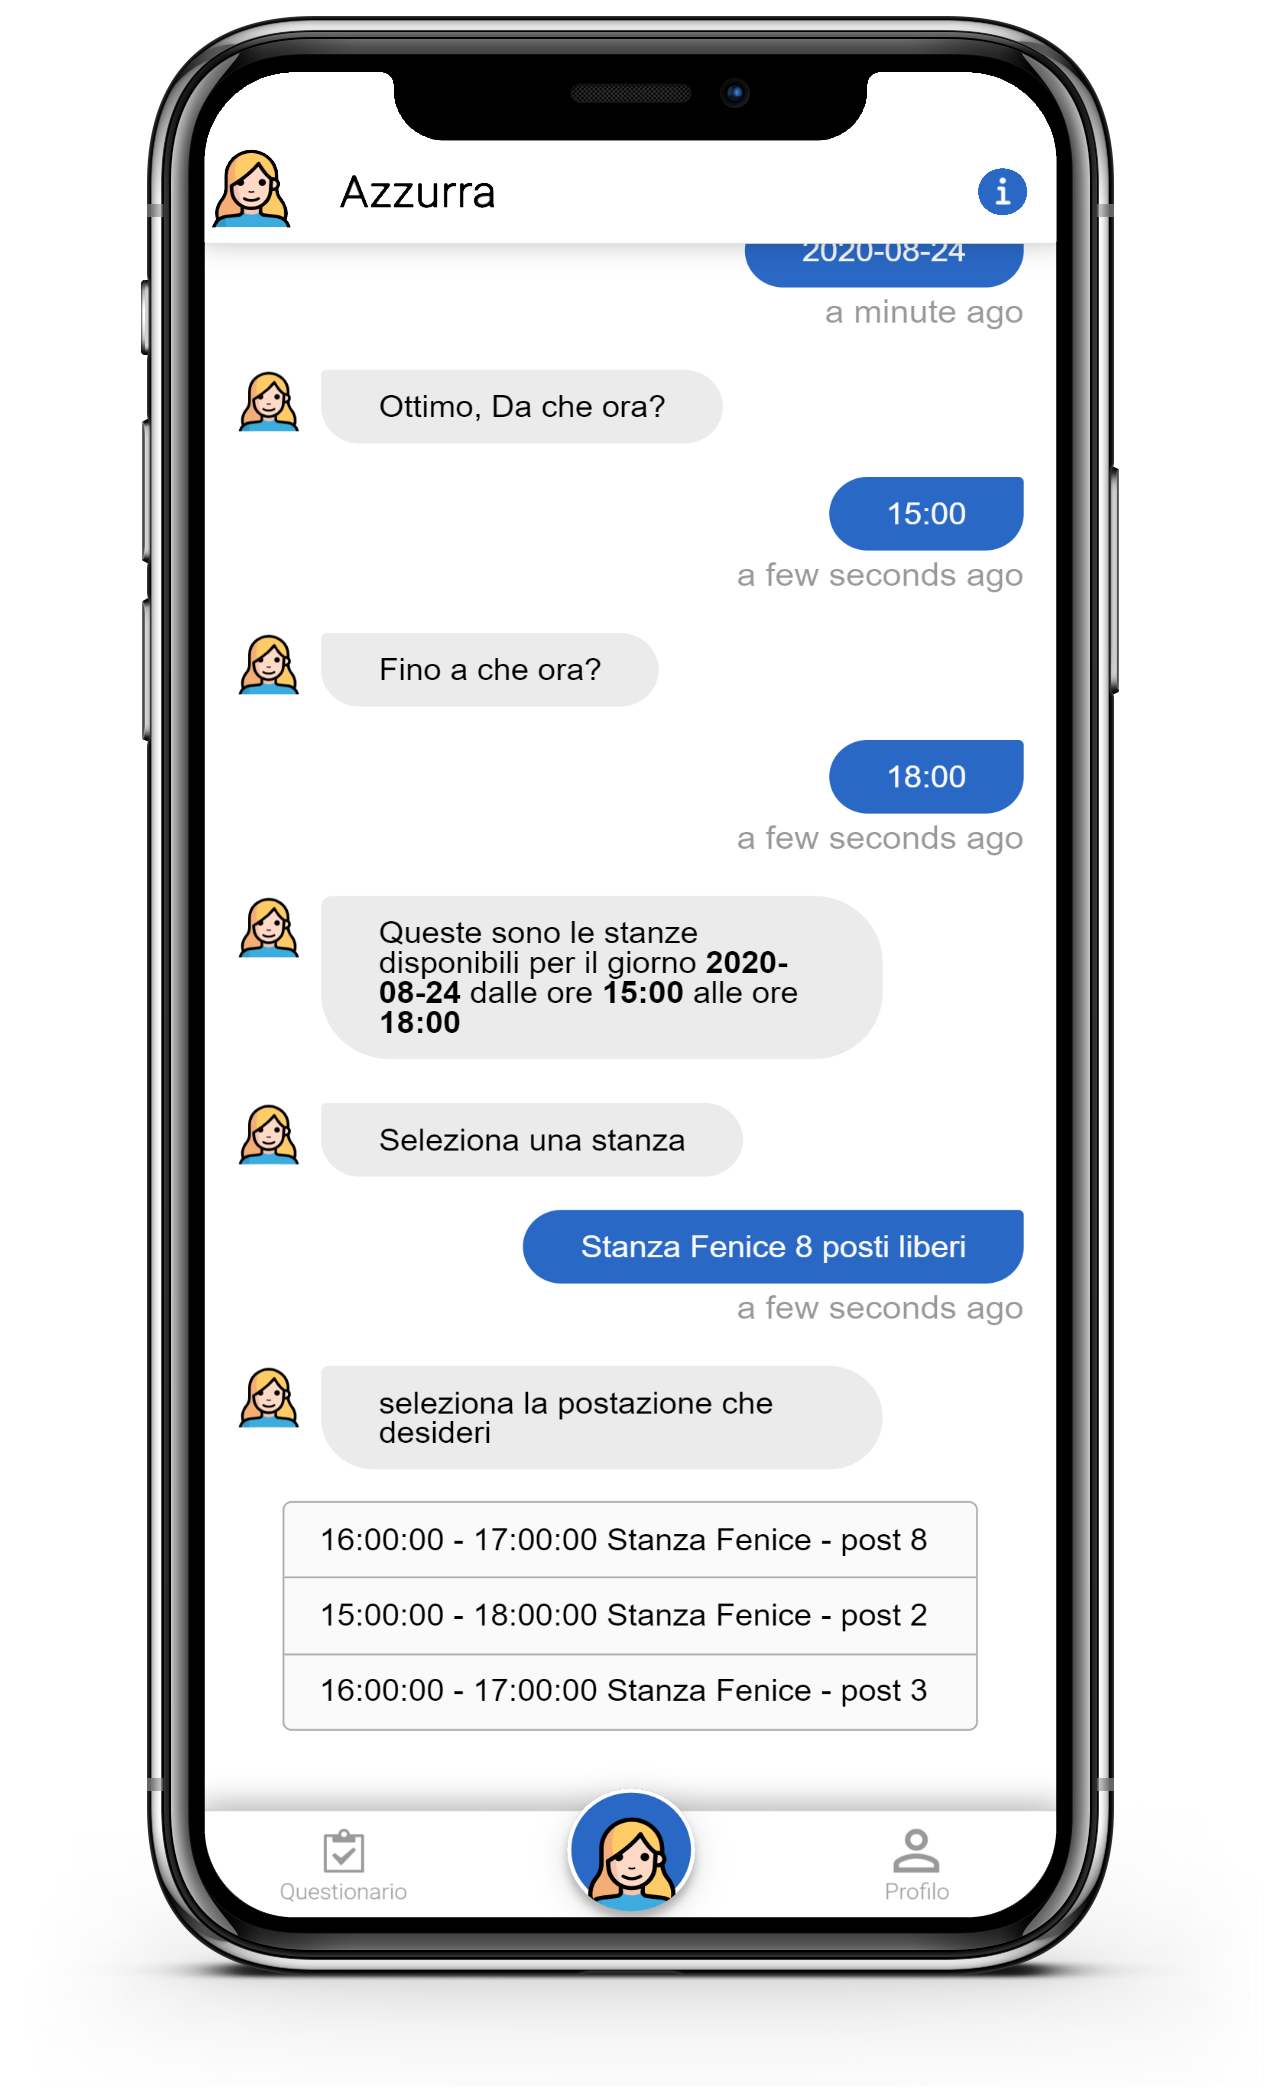
\includegraphics[scale=0.167]{DB2.png}\hfill
		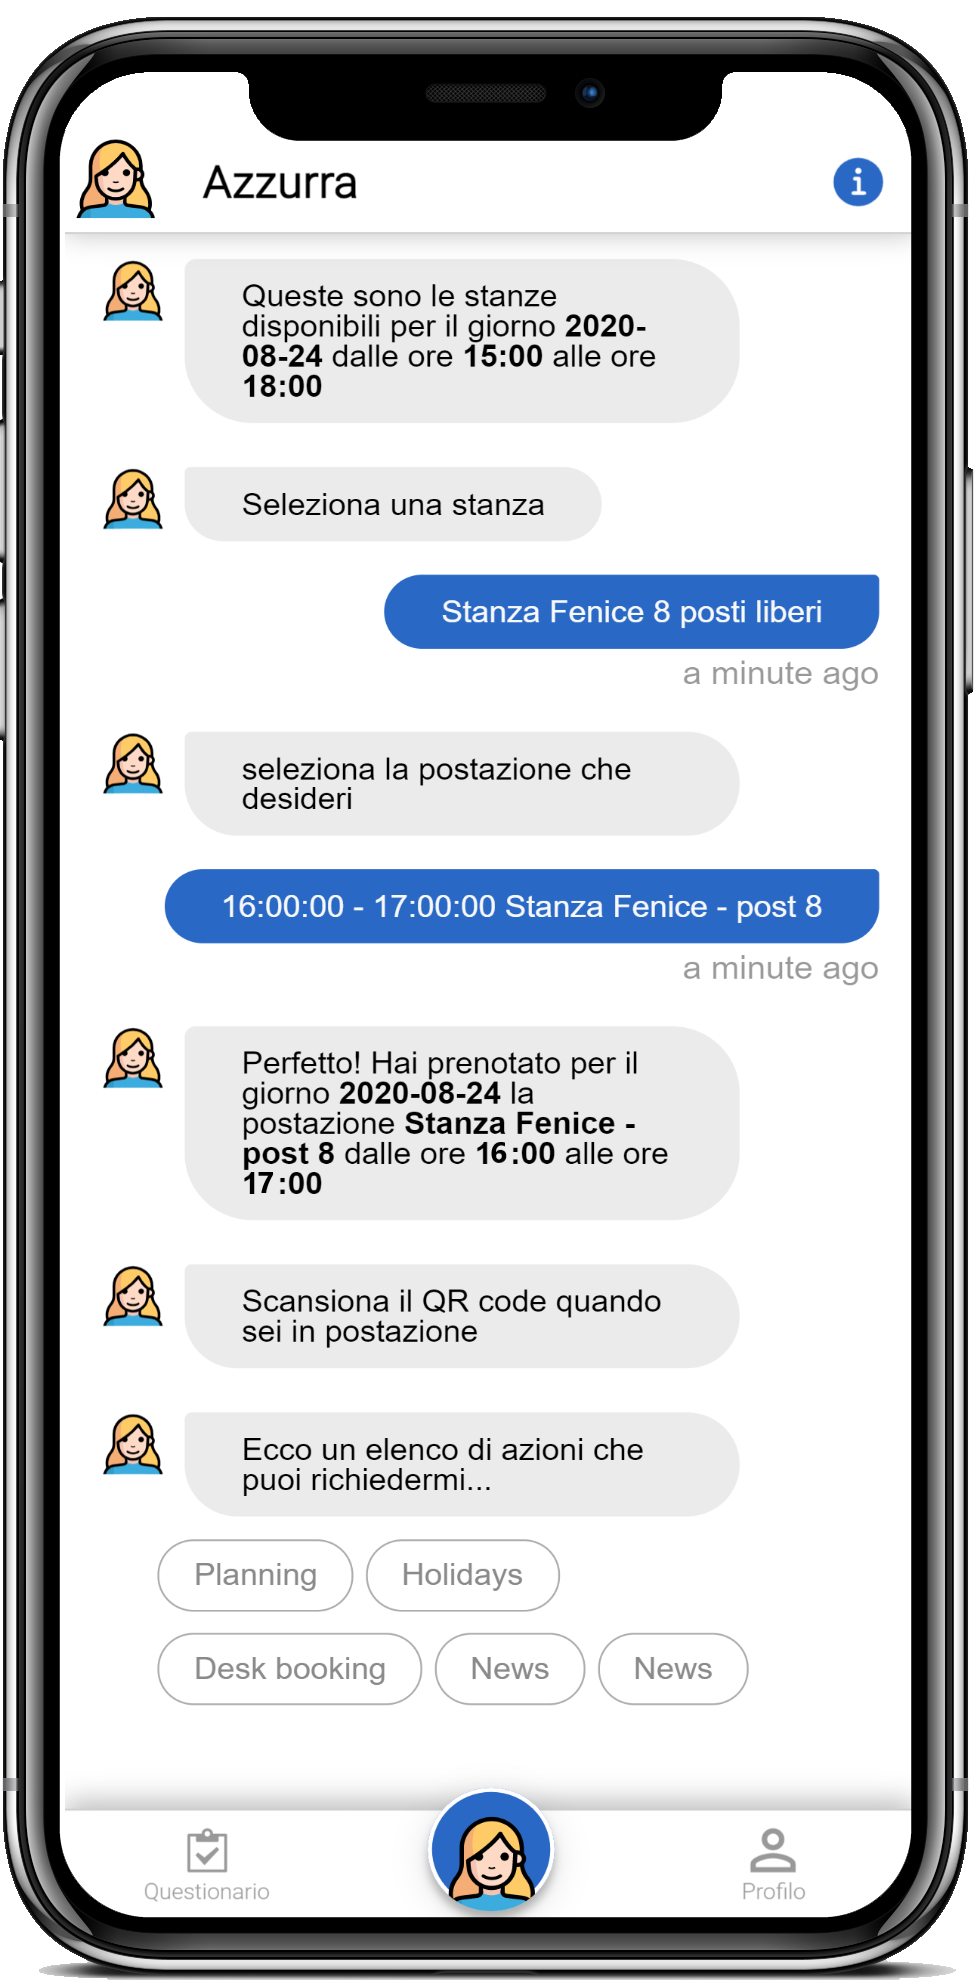
\includegraphics[scale=0.167]{DB3.png}
		\caption{Richiesta di inserimento di una nuova prenotazione}\label{fig:DB}
	\end{center}
\end{figure}
\clearpage
Nella Figura~\ref{fig:QRc} viene mostrata la \emph{chat} tra Azzurra e l'utente per la richiesta di inserimento di una nuova prenotazione. Viene perciò richiesto il giorno e l'intervallo di tempo in cui fare la prenotazione, viene chiesto in quale stanza deve essere il posto da prenotare e infine, viene chiesto quale posto a sedere vuole prenotare tra quelli disponibili secondo i parametri inseriti dall'utente.

\section{Considerazioni}
I risultati ottenuti hanno soddisfatto tutti i requisiti stabili e sono stati soddisfacenti per il tutor aziendale. Dai risultati precedentemente elencati si sono fatte delle considerazioni su come essi potessero essere migliorati in termini di \emph{user experience}. Come scritto l'\g{architettura} che supporta Azzurra permette di tenere lo storico dei messaggi e lo stato della conversazione, per una certa durata, in modo da rendere migliore l'interazione tra utente e Azzurra. Un ulteriore miglioramento che può essere adottato è l'introduzione dei comandi vocali. Al momento l'inserimento dei dati da parte dell'utente avviene tramite comandi \emph{touch} cioè, l'utente tocca sullo schermo l'opzione che desiderata. Avvolte l'interazione tramite comandi \emph{touch} può risultare limitante per alcuni utenti ad'esempio persone con limitazioni alla vista oppure banalmente il \emph{device} dell'utente in cui c'è applicazione \emph{mobile} risulta essere troppo piccolo e l'utente ha difficoltà a premere i bottini giusti insomma, persone che per qualsiasi motivo hanno l'impossibilità o la difficoltà a usare le mani per inserire le loro scelte. Grazie ai comandi vocali queste persone riuscirebbero a interagire con Azzurra facilmente sostituendo l'uso delle mani con l'uso della voce. \\

Dalla possibile introduzione dei comandi vocali nascono però altre considerazione. Il riconoscimento vocale deve essere sufficientemente accurato da capire ciò che dice l'utente perché altrimenti può provocare una sensazione negativa di irritazione o frustrazione nell'utente dovuta al fatto che ciò che dice non viene capito dall'applicazione e quindi non offrire una buona \emph{user experience}. In sintesi un possibile modo per migliorare l'\emph{user experience} dell'applicazione è l'introduzione dei comandi vocali ma, tale introduzione deve essere ben implementata valutandone i rischi e costi da affrontare.

             % Product Prototype
% !TEX encoding = UTF-8
% !TEX TS-program = pdflatex
% !TEX root = ../tesi.tex

%**************************************************************
\chapter{Testing}
\label{cap:test}
%**************************************************************
\intro{Nel seguente capitolo verranno descritte le tecnologie utilizzate per costruire una test-suite per l'applicazione \emph{mobile} e verrà esposto il piano di \emph{test} stabilito con il tutor aziendale, inserendo i risultati ottenuti.}
\section{Test End to End}
Il \emph{test End-to-End} è una metodologia di \emph{testing} dell'interfaccia grafica che viene vista dagli utenti dell'applicazione. Ha lo scopo di testare in modo automatizzato se, tutti flussi di esecuzione dell'applicazione, dall'inizio fino alla fine, si stanno comportando come progettato, senza che vengano rilevati degli errori che andrebbero a inficiare sulla qualità dell’applicazione stessa. Perciò il \emph{test} \gls{test e2e} consiste nel simulare degli scenari utente reali ad esempio interazioni attraverso \emph{clic} sui bottoni da parte degli utenti, in modo da verificare che l'applicazione si comporti nel modo corretto garantendo che vengano soddisfati i requisiti di alto livello del prodotto. Inoltre, il \emph{test} \gls{test e2e} verifica che l'intera applicazione su tutte le possibili interazione che l'utente può fare, vengono trasmesse le informazioni corrette tra le varie componenti dell'applicazione garantendo che l'applicazione funzioni come un unico sistema coerente. Un esempio di \emph{test} \gls{test e2e} possono essere la simulazione dei passi che l'utente deve fare per autenticarsi nell'applicazione, quindi il \emph{test} può essere così composto:
\begin{enumerate}
	\item Inserisci l'\emph{username} nella casella di testo;
	\item Inserisci la \emph{password} nella casella di testo;
	\item Clicca il bottone di \emph{login};
	\item Verifica che ti trovi nella pagina principale dell'applicazione dopo l'autenticazione e non più nella pagina di \emph{login}.
\end{enumerate}

Come scritto, i \emph{test} \gls{test e2e} eseguono l'applicazione proprio come se fosse un utente in un ambiente il più vicino possibile alla realtà. Proprio come un utente, i \emph{test} \gls{test e2e} dovrebbero avere una comprensione praticamente nulla dei componenti interni dell'applicazione perché si vuole evitare accoppiamenti non necessari. Infatti, i test di unità e di integrazione sono i luoghi in cui dovrebbe essere nota la composizione interna dell'applicazione, e quindi dove i \g{mock} possono essere utilizzati per attivare particolari rami di codice che si ha l'esigenza di testare. Il fatto che i \emph{test} \gls{test e2e} non sanno la struttura interna e il funzionamento dell'applicazione che stanno testando li classifica come \emph{test} \emph{black-box}.
\clearpage

\begin{figure}[!h] 
	\begin{center}
		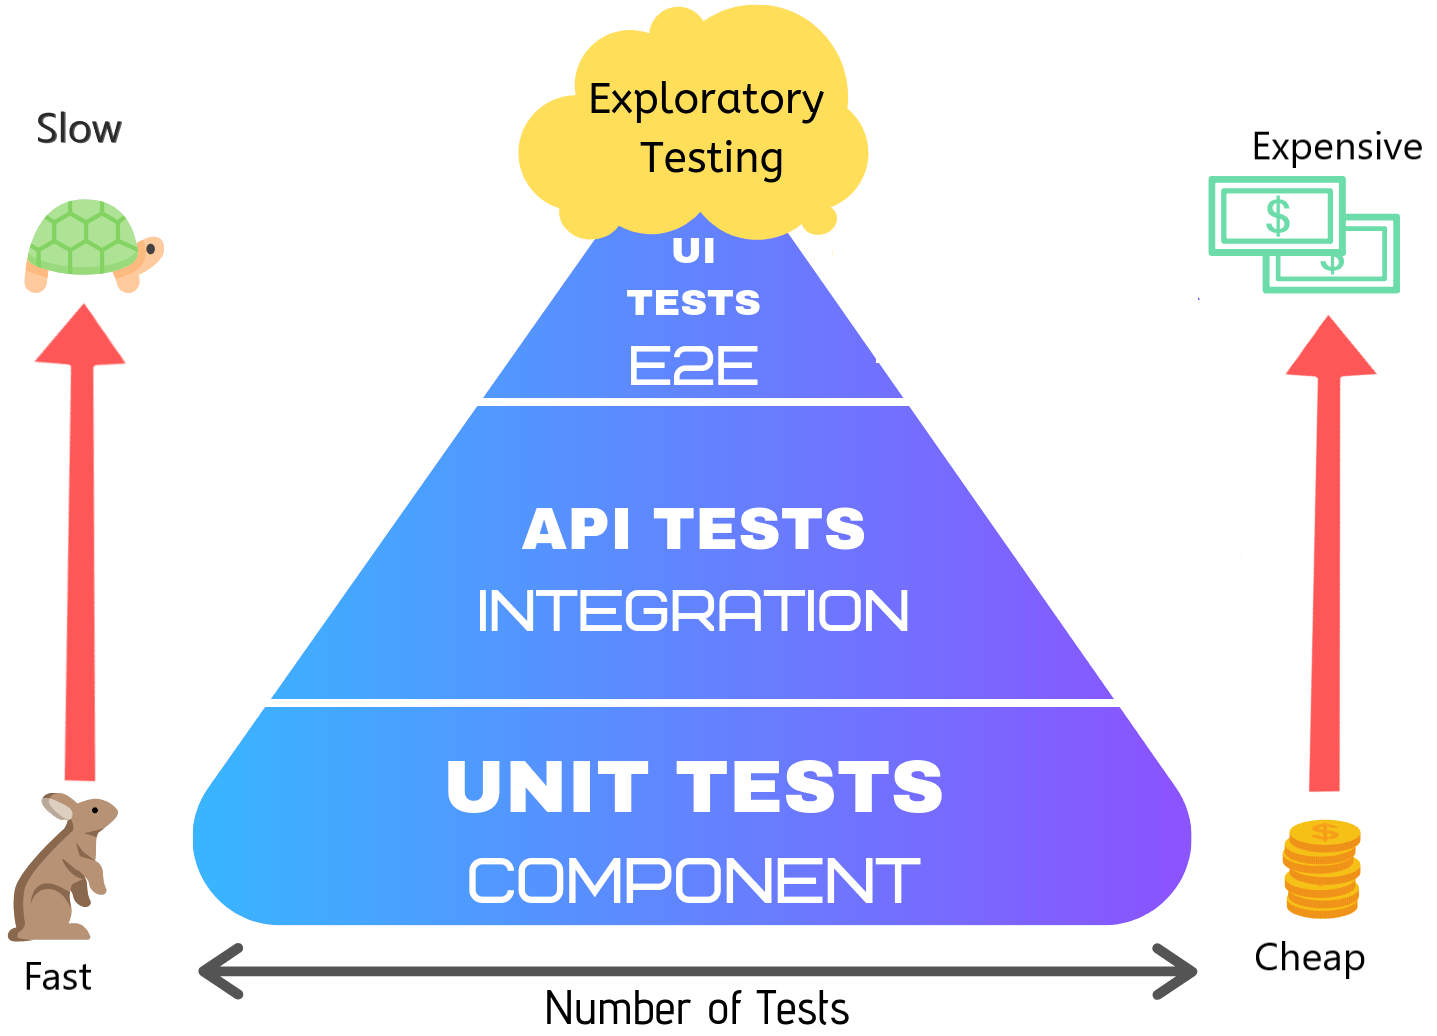
\includegraphics[scale=0.3]{piramideTest.png}
		\caption{Piramide dei test}\label{fig:test}
	\end{center}
\end{figure}

Come mostra la Figura~\ref{fig:test}, la piramide dei \emph{test} illustra il numero proporzionale di \emph{test} per ogni tipologia di \emph{test} in relazione alla loro velocità d'esecuzione e costi per implementarli. Sebbene i \emph{test} \gls{test e2e} forniscano un grande supporto per testare la correttezza dell'applicazione, sono significativamente più lenti e più costosi rispetto ai test unitari, a causa della loro elevata complessità e onerosità computazionale. Perciò è fondamentale trovare il giusto equilibrio di \emph{test} \gls{test e2e} da implementare senza perderne i vantaggi e senza aumentare i costi per l'implementazione. Una buona applicazione di \emph{test} \gls{test e2e} può essere ad esempio il \emph{testing} di azioni ripetitive che grazie alla fatto che sono \emph{test} automatizzati, risultano essere meno costosi è più efficaci rispetto ai \emph{test} manuali.

\section{Tecnologie per il testing}
Per implementare i \emph{test} \gls{test e2e} sia per la \emph{dashboard} di \gls{AWMS} sia per l'applicazione \emph{mobile} si sono usare diverse tecnologie tra loro. Per il \emph{testing} della \emph{dashboard} si sono usate le seguenti tecnologie:
\begin{itemize}
	\item \textbf{Selenium WebDrive};
	\item \textbf{Protractor};
	\item \textbf{Cucumber}.
\end{itemize}
Selenium è un \g{framework} che permette di automatizzare l'esecuzione dei \emph{test} all'interno dei \g{browser web}. Ciò è possibile grazie a un insieme di \g{api} detto API WebDriver. Queste \g{api} sono uno standard \gls{W3C} che rappresentano un'interfaccia di controllo remoto che consente di manipolare elementi del \g{DOM} nelle pagine web e di comandare il comportamento dei programmi utente. Inoltre, fornisce un protocollo, noto come JSON Wire Protocol, per il trasferimento dei dati per varie piattaforme che permettono di automatizzare i \emph{test} sui \g{browser web} come:
\begin{itemize}
	\item GeckoDriver per Mozilla Firefox;
	\item ChromeDriver per Google Chrome;
	\item SafariDriver per Apple Safari;
	\item InternetExplorerDriver per Microsoft Internet Explorer;
	\item MicrosoftWebDriver o EdgeDriver per Microsoft Edge;
	\item OperaChromiumDriver per Opera.
\end{itemize}
Selenium per eseguire i \emph{test} utilizza un’architettura client-server infatti, Selenium utilizza un \g{server} web dove espone l'API WebDriver come \gls{api} \g{rest}. Perciò rimane in ascolto per la ricezione dei comandi che compongono i \emph{test}, sotto forma di richieste \g{http}. Quando arrivano le richieste le esegue su un \g{browser web} e risponde con una risposta \g{http} che rappresenta il risultato dell'esecuzione del comando. Grazie alla standardizzazione delle \g{api} e l'utilizzo di un architettura client-server è possibile eseguire \emph{test} scritti in diversi linguaggi purché supportino l'invio di richieste \g{http}.\\

Protractor è un \g{framework} di \emph{test} \gls{test e2e} per applicazioni Angular2+ e AngularJS. Protractor offre un insieme di "localizzatori" cioè metodi che permettono di ricavare gli elementi o il valore degli attributi dall'applicazione web, ma anche di simulare dei \emph{click} come se fosse un utente umano. Per funzionare Protractor all'inizio richiede che sia presente un server Selenium in modo da mandare richieste \g{http} per eseguire i \emph{test} \gls{test e2e}.\\

\begin{figure}[h] 
	\begin{center}
		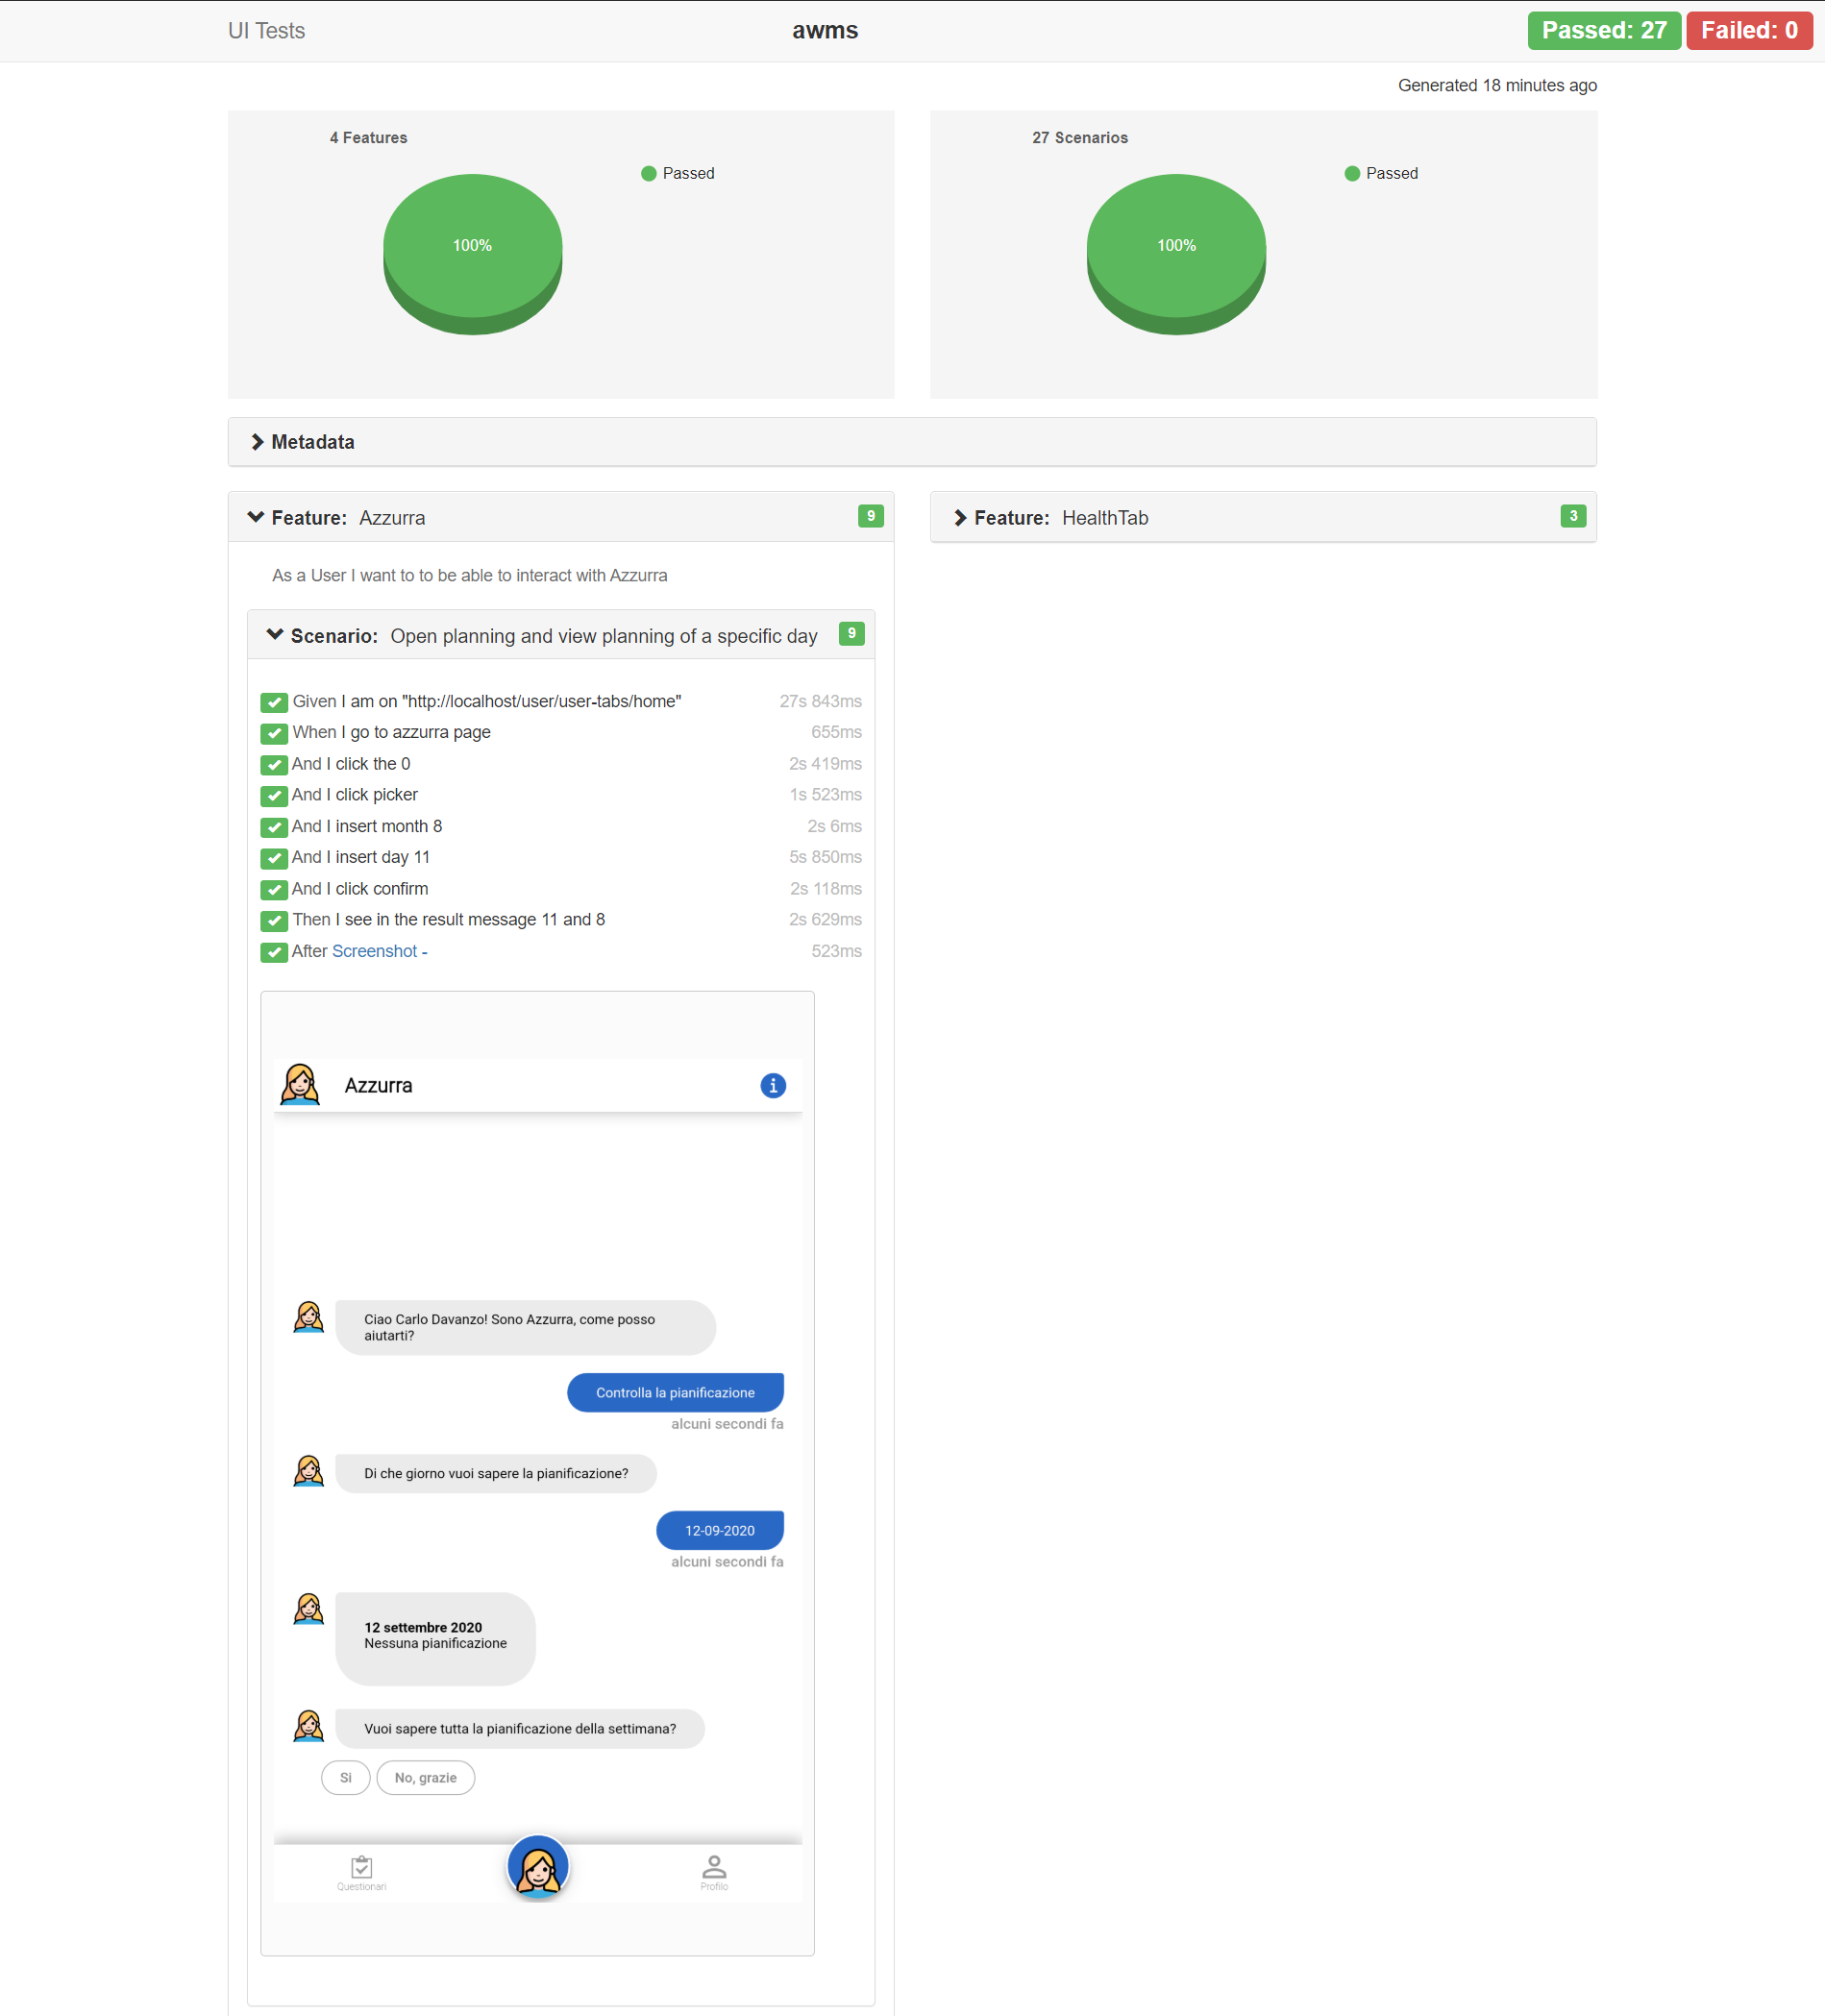
\includegraphics[height=20cm, width=13cm]{report.png}
		\caption{Una parte del report dei test per il mobile generato da Cucumber}\label{fig:testDoc}
	\end{center}
\end{figure}

Infine, Cucumber permette di definire i vari passi che deve fare un \emph{test} automatizzato per simulare le azioni di un utente. Questi passi vengono dichiarati attraverso il linguaggio Gherkin. Quindi grazie a Cucumber vengono dichiarati i cosiddetti \emph{step} cioè i passi che devono essere fatti all'interno del \emph{test}, l'insieme dei \emph{step} definisce lo scenario dei \emph{test}, ad esempio uno scenario di \emph{test} può essere il processo di autenticazioni e gli \emph{step} sono l'inserimento dei dati e l'invio. I vari \emph{step} vengono poi implementati in un linguaggio di programmazione, in questo caso TypeScript utilizzando i metodi offerti da Protractor. Il fatto che vengano dichiarati i passi che il \emph{test} permettono a Cucumber di supportare la \gls{BDD}. Quando vengono eseguiti i \emph{test} Cucumber controlla se Selenium sta eseguendo le azioni specificate all’interno di un \g{browser web}. Al termine dell'esecuzione Cucumber riesce a stabilire l'esito per ogni \emph{test} inoltre, produce dei \emph{report} sui \emph{test} appena eseguiti documentandone l'esito e la struttura come mostrato in Figura~\ref{fig:testDoc}.
\clearpage
Per l'applicazione \emph{mobile} si è continuato a utilizzare Protractor e Cucumber ma al posto di Selenium si è utilizzato Appium. Viene utilizzato Appium perché offre l'automazione dei \emph{test} per \glslink{applicazione nativa}{applicazioni native}\textcolor{SchoolColor}{\ap{[g]}}, \glslink{applicazione web mobile}{applicazioni web mobile}\textcolor{SchoolColor}{\ap{[g]}} e \glslink{applicazione ibrida}{applicazioni ibride}\textcolor{SchoolColor}{\ap{[g]}}, con la particolarità di essere multi-piattaforma cioè può eseguire i \emph{test} sia su \g{iOS} e \g{Android}. Selenium invece non permette l'esecuzione di \emph{test} su dispositivi \emph{mobile} ma solo su \g{browser web}. Appium utilizza la stessa architettura client-server di Selenium inoltre da esso ne prende anche l'utilizzo dell'API WebDriver in particolare viene utilizzato una variante per il \emph{mobile} del protocollo JSON Wire Protocol noto con il nome di Mobile JSON Wire Protocol. 

\begin{figure}[h] 
	\begin{center}
		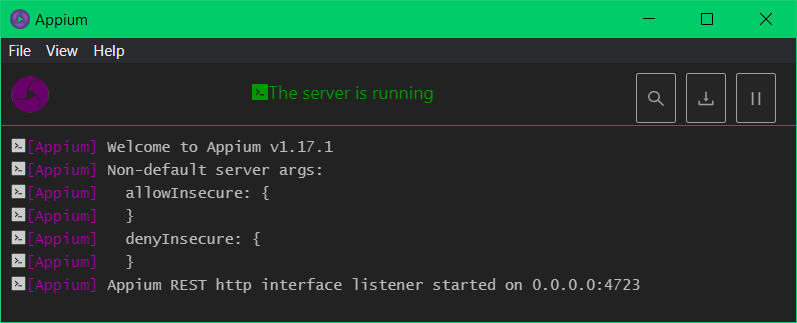
\includegraphics[scale=0.5]{appiumServer.png}
		\caption{Schermata del server Appium}\label{fig:appiumServer}
	\end{center}
\end{figure}

Di conseguenza Appium permette di utilizzare qualsiasi linguaggio o \g{framework} che supporti l'invio di richieste \g{http} inoltre, non è necessario compilare alcun codice o \g{framework} specifico di Appium perché grazie al Mobile JSON Wire Protocol utilizza i \g{framework} per l'automazione dei \emph{test} come UIAutomator per\g{Android} e XCTest per \g{iOS}.


\section{Convezione}
Su suggerimento del tutor aziendale si è struttura la \emph{test-suite} da me implementata nel seguente modo:\\
\begin{center}
	\begin{forest}
		for tree={font=\sffamily, grow'=0,
			folder indent=.9em, folder icons,
			edge=densely dotted}
		[e2e
		[test%, this folder size=20pt
		[feature%, this folder size=20pt
		[spec.feature, is file]
		]
		[step\_definition%, this folder size=20pt
		[spec.e2e-spec.ts, is file]
		]
		[pages%, this folder size=20pt
		[specs.po.ts, is file]
		]
		]
		]
	\end{forest}
\end{center}
\begin{itemize}
	\item \textbf{feature}: Contiene i file.feature dove vengono indicati gli scenari e gli \emph{step} dei \emph{test} scritti nell'linguaggio Gherkin. Ogni file.feature contiene \emph{test} di scenari affini;
	\item \textbf{step\_definition}: Contiene i file.e2e-spec.ts dove vengono implementati gli \emph{step}, utilizzando i metodi dei file.po.ts. Esiste un file.e2e-spec.ts per ogni file.feature;
	\item \textbf{pages}: Contiene le cosiddette PageObject, le PageObject sono un \g{design pattern} che permettono di scrivere \emph{test} più puliti. Infatti, queste PageObject contengono metodi che vengono spesso riutilizzati da più \emph{test} e inoltre, contiene metodi che estraggono gli elementi dalla vista. Adottando questo \g{design pattern} si ha il vantaggio che se il modello dell'applicazione cambia sarà sufficiente aggiornare solo la PageObject e inoltre si ha il vantaggio di non avere duplicazione del codice. Solitamente si creano più PageObject con metodi tra loro affini.
\end{itemize}
\section{Test eseguiti}
In comune accordo con il tutor aziendale, sono stati individuati i seguenti \emph{test} \gls{test e2e} che debbano testare l'intera applicazione \emph{mobile} quindi, non solo Azzurra ma anche le sezioni Questionario e Profilo. Inoltre sono stati testati anche alcuni aspetti della \emph{dashboard} di \gls{AWMS}. Per ogni \emph{test} viene assegnato un codice composto dalla lettera \textbf{T}, da una seconda lettera che può essere \textbf{M} nel caso in cui il \emph{test} sia per l'applicazione \emph{mobile}, oppure la lettera \textbf{D} se il \emph{test} è per la \emph{dashboard}. Infine il codice termina con un numero progressivo. Nella tabella sottostante per ogni \emph{test} viene riportato il suo codice, una descrizione e l'esito del \emph{test}.
\begin{table}[h]%
	\rowcolors{2}{grigetto}{white}
	\renewcommand{\arraystretch}{1.4}
	\centering
	\begin{tabularx}{\textwidth}{c X c}
		\hline	
		\rowcolor{heavenly}
		\intest{Codice} &  \intest{Descrizione} & \intest{Esito}\\	
		\hline			
		TM1 & Testare che l'utente possa inserire \emph{e-mail} e \emph{password} e cliccare il bottone invio per autenticarsi, nel caso i dati siano corretti l'utente deve essere renderizzato nella pagina Questionari. & Superato\\
		TM2 & Testare che l'utente possa inserire\emph{e-mail}, \emph{password} e cliccare il bottone invio per autenticarsi, nel caso i dati siano uno o tutti errati l'utente deve essere rimanere nella pagina di autenticazione. & Superato\\
		TM3 & Testare che nel caso in cui esista una versione più recente rispetto a quella in esecuzione, appaia all'apertura dell'applicazione un messaggio in primo piano che avvisi della nuova versione disponibile. & Superato\\
		TM4 & Testare che il messaggio in primo piano che avvisa della nuova versione disponibile, sia interagitile, cioè che si possa cliccare i suoi bottoni. & Superato\\
		TM5 & Testare che una volta che l'utente sia autenticato, se è il suo primo accesso, possa chiudere la finestra che contiene la guida per l'utilizzo dell'applicazione, la quale appare al primo accesso che si fa nell'applicazione. & Superato\\
		TM6 & Testare nella sezione Questionari, se la prima finestra del Questionario della salute (vedi la prima immagine della Figura~\ref{fig:queSlide}) abbia i vari bottoni dei sintomi tutti cliccabili. & Superato\\
		\hline
	\end{tabularx} \hbox{}
	\caption{Tabella del tracciamento dei test E2E}
\end{table}%	
	
\begin{table}[h]%
	\renewcommand{\arraystretch}{1.4}
	\rowcolors{2}{grigetto}{white}
	\centering
	\begin{tabularx}{\textwidth}{c X c}
		\hline	
		\rowcolor{heavenly}
		\intest{Codice} &  \intest{Descrizione} & \intest{Esito}\\	
		\hline	
		TM7 & Testare nella sezione Questionari, se la seconda finestra del Questionario della salute (vedi la seconda immagine della Figura~\ref{fig:queSlide}) abbia i vari bottoni sulla salute delle persone che vivono con te, siano tutti cliccabili. & Superato\\
		TM8 & Testare nella sezione Questionari, se la terza finestra del Questionario della salute (vedi la terza immagine della Figura~\ref{fig:queSlide}) abbia i vari bottoni dei posti in cui sei stato, siano tutti cliccabili. & Superato\\
		TM9 & Testare nella sezione Questionari, che venga visualizzato esito positivo(vedi prima immagine della Figura~\ref{fig:quefinal}) dalla compilazione del questionario se l'indice di contagiosità calcolato è basso. & Superato\\
		TM10 & Testare nella sezione Questionari, che venga visualizzato esito negativo(vedi seconda immagine della Figura~\ref{fig:quefinal}) dalla compilazione del questionario se l'indice di contagiosità calcolato è alto. & Superato\\
		TM11 & Testare nella sezione profilo che tutti i bottoni presenti siano cliccabili e che aprano la loro corrispondente finestra. & Superato\\
		TM12 & Testare nella sezione profilo, nella finestra Informazioni personali, se la ricerca degli indirizzi, per poter cambiare indirizzo di domicilio, produca risultati coerenti con quello che si sta cercando. & Superato\\
		TM13 & Testare nella sezione profilo, nella finestra Informazioni, si possa selezionare uno dei risultati della ricerca per il cambio dell'indirizzo di domicilio & Superato\\
		TM14 & Testare nella sezione profilo, nella finestra Informazioni, che tutti i bottoni siano cliccabili & Superato\\
		TM15 & Testare nella sezione profilo, nella finestra Informazioni, che le modifiche fatte a i dati una volta cliccato il bottone salva, rimangano salvate anche dopo la chiusura della finestra & Superato\\
		TM16 & Testare nella sezione profilo, Gestione password, si possa cambiare la \emph{password} quindi che si possa inserire la \emph{password} attuale, inserire una nuova \emph{password}, la sua conferma e cliccare sul bottone salva. & Superato\\
		TM17 & Testare nella sezione profilo, che tutte le finestre aperte dopo il \emph{click} sui bottoni, possano essere chiuse. & Superato\\
		TM18 & Testare nella sezione Azzurra, nella funzionalità "pianificazione" si possa visualizzare la pianificazione in uno specifico giorno. & Superato\\
		TM19 & Testare nella sezione Azzurra, nella funzionalità "Pianificazione" si possa visualizzare la pianificazione della settimana corrente. & Superato\\
		TM20 & Testare nella sezione Azzurra, nella funzionalità "Gestione assenze" si possa richiedere l'inserimento di una nuova assenza. & Superato\\
		\hline
	\end{tabularx} \hbox{}
	\caption{Tabella del tracciamento dei test E2E}
\end{table}%

\begin{table}[h]%
	\rowcolors{2}{grigetto}{white}
	\renewcommand{\arraystretch}{1.6}
	\centering
	\begin{tabularx}{\textwidth}{c X c}
		\hline	
		\rowcolor{heavenly}
		\intest{Codice} &  \intest{Descrizione} & \intest{Esito}\\	
		\hline	
		TM21 & Testare nella sezione Azzurra, nella funzionalità "Gestione assenze" si possa visualizzare la lista delle assenze fatte. & Superato\\
		TM22 & Testare nella sezione Azzurra, nella funzionalità "Gestione assenze" si possa aprire il calendario dei giorni in cui si può prendere un permesso. & Superato\\
		TM23 & Testare nella sezione Azzurra, nella funzionalità "Prenotazione posto" che, si possa visualizzare le prenotazioni dei posti a sedere fatte. & Superato\\
		TM24 & Testare nella sezione Azzurra, nella funzionalità "Prenotazione posto" che, si possa inserire una nuova prenotazione di un posto a sedere. & Superato\\
		TM25 & Testare nella sezione Azzurra, nella funzionalità "Prenotazione posto" che, si possa aprire lo scanner di \g{QR code}\. & Superato\\
		TM26 & Testare nella sezione Azzurra, che si possa aprire il menu delle shortcuts. & Superato\\
		TM27 & Testare che siano raggiungibili le sezioni Questionari, Azzurra, Profilo, dopo l'autenticazioni. & Superato \\
		TD28 & Testare nella sezione Task che all'inizio non ci sia nessun \emph{task} selezionato. & Superato \\
		TD29 & Testare nella sezione Task che tutti i \emph{task} siano selezionabili. & Superato \\
		TD30 & Testare nella sezione Task che una volta selezionato un \emph{task}, appaia a lato un menu a tendina. & Superato \\
		TD31 & Testare nella sezione Task che la funzionalità di ricerca produca risultati coerenti con quanto si sta cercando. & Superato \\
		TD32 & Testare nella sezione Safety che tutti i bottoni siano cliccabili e nel caso in cui aprano delle nuove finestre, queste possano essere chiuse. & Superato \\
		TD31 & Testare nella sezione Safety che la funzionalità di ricerca produca risultati coerenti con quanto si sta cercando. & Superato \\
		\hline
	\end{tabularx} \hbox{}
	\caption{Tabella del tracciamento dei test E2E}
\end{table}%
\clearpage
\section{Considerazioni}
I \emph{test} prodotti sono stati in linea con quanto chiesto del tutor aziendale. Dall'esperienza vissuta sull'implementazione dei \emph{test} \gls{test e2e} si sono fatte delle considerazioni su di essi. Dopo un iniziale difficoltà nell'implementazione dei \emph{test} dovuta alla natura asincrona dei \emph{test} cioè i \emph{test} fallivano perché erano più veloci ad eseguirsi rispetto alla renderizzazione delle componenti grafiche che dovevano testare, ad esempio un \emph{test} non trovava una componente grafica perché non aspettava che fosse renderizzata e falliva anche se la componente grafica c'era. Si è quindi capito quanto fosse molto oneroso in termini di tempo spesi per implementare i vari \emph{test} \gls{test e2e} ciononostante, grazie all'utilizzo delle PageObject e dei loro metodi è stato risparmiato del tempo riutilizzando i metodi implementati precedentemente.\\

da quanto si è fatto, si è capito quanto siano costosi i \emph{test} \gls{test e2e} non solo da essere implementati ma anche per eseguirli, infatti per eseguire solo ventisette \emph{test} per il \emph{mobile} si è impiegato più di quindici minuti mentre con l'aggiunta dei \emph{test} per la \emph{dashboard} si è arrivati a più di venti minuti.\\

Infine un aspetto critico rilevato è stato il fatto che alcuni casi non possono essere testati o se ci si prova richiedono troppo tempo per essere testati, ad esempio non è stato possibile verificare in modo completamente automatizzato se lo \emph{scanner} di \g{QR code} fosse in grado di funzionare correttamente, questo perché non si poteva generare un \g{mock} di \g{QR code} da mostrare. Si poteva comunque fare un \emph{test} semi automatizzato, cioè quando il \emph{test} apriva la fotocamere per scannerizzare, si mostrare manualmente un \g{QR code} cosi che lo \emph{scanner} riusciva a scansionare e a verificare se tutto funzionava correttamente.\\

Si considera perciò che i \emph{test} \gls{test e2e} danno un grande valore aggiunto nella qualità del prodotto ma questi vanno usati per testare operazioni ripetitive e che possano essere da \emph{test} facilmente implementabili perché in alcuni casi non conviene implementare dei \emph{test} \gls{test e2e} completamente automatizzati.             % Product Design Freeze e SOP
% !TEX encoding = UTF-8
% !TEX TS-program = pdflatex
% !TEX root = ../tesi.tex

%**************************************************************
\chapter{Conclusioni}
\label{cap:conclusioni}
%**************************************************************

%**************************************************************
\section{Consuntivo finale}
Rispetto al piano di lavoro pianificato esposto nella sezione \hyperref[cap:pianificazione]{§2.5}, sono avvenute delle modifiche e degli scostamenti. Ciononostante, il progetto di stage si è concluso soddisfacendo gli obbiettivi e i prodotti richieste e pianificati. Nonostante le ore totali pianificate inizialmente erano di trecentoventi ore, tutte le attività pianificate si sono concluse con due giorni d'anticipo, perciò il totale di ore svoltesi è stato di trecentoquattro. Ciò significa che la nona settimana non è stato svolta essendosi concluso prima lo stage. Nella prima settimane c'è stato uno scostamento di dodici ore questo perché lo studio approfondito delle tecnologie da utilizzare ha richiesto più tempo del previsto. Nella seconda settimana su decisione del tutor aziendale, si è spostato l'implementazione dei \emph{test} \gls{test e2e} per il \emph{mobile} nella sesta settimana applicando l'attività testando tutte le funzionalità dell'applicazione \emph{mobile} e non solo alcune funzionalità come era stato pianificato inizialmente. Nella terza settimana sono state richieste quattro ore in più a causa di un \emph{bug} manifestatosi di QR Scanner, ciononostante è stato egregiamente gestito e risolto. Nella quarta e quinta settimana si sono risparmiate per ogni settimana otto ore. Nella sesta settimana si è aggiunto l'implementazione dei \emph{test} \gls{test e2e} per il \emph{mobile} questo perché non è stato possibile effettuare l'implementazione delle \glslink{notifica push}{notifiche push}\textcolor{SchoolColor}{\ap{[g]}} a causa di esigenze aziendali cioè, l'azienda aveva l'esigenza di avere già subito implementate le \glslink{notifica push}{notifiche push}\textcolor{SchoolColor}{\ap{[g]}}, cosi sono state implementante dai membri dell'azienda. L'attività è stata sostituita dall'attività di documentazione delle \glslink{notifica push}{notifiche push}\textcolor{SchoolColor}{\ap{[g]}} oltre all'attività di \emph{testing}.
Nella ottava settimana sono state richieste meno ore di quanto pianificato risparmiando cosi otto ore.
Di seguito viene mostrata la tabella riportante il consuntivo finale del progetto di stage.

\begin{table}[h]%
	\rowcolors{2}{grigetto}{white}
	\renewcommand{\arraystretch}{1.7}
	\centering
	\begin{tabularx}{\textwidth}{X c c c}
		\hline	
		\rowcolor{heavenly}
		\intest{Attività} & \intest{Ore Pianificate} & \intest{Ore Effettive} & \intest{Scostamento}\\	
		\hline			
		Studio delle tecnologie, Angular 2+ e Ionic, da utilizzare durante lo stage & 24 & 36 & 12 \\
		
		Studio di componenti del dell'architettura di sistema di Azzurra, creazione di \emph{test} per la \emph{dashboard} di \gls{AWMS} e per l'applicazione \emph{mobile} & 40 & 40 & 0 \\
\end{tabularx} \hbox{}

\caption{Tabella riassuntiva del consultivo delle attività per il progetto di stage}
\end{table}
		
\begin{table}[h]%
	\rowcolors{2}{grigetto}{white}
	\renewcommand{\arraystretch}{1.7}
	\centering
	\begin{tabularx}{\textwidth}{X c c c}
		\hline	
		\rowcolor{heavenly}
		\intest{Attività} & \intest{Ore Pianificate} & \intest{Ore Effettive} & \intest{Scostamento}\\	
		\hline		
		Continuazione studio delle componenti del sistema di Azzurra e analisi, progettazione e implementazione di flussi conversazionali. & 40 & 44 & +4 \\
		
		Scritture di documentazione per le componenti di Azzurra. & 40 & 32 & -8\\
		
		Continuazione studio di altre componenti di \gls{AWMS}. & 40 & 32 & -8\\
		
		Documentazione delle componenti \gls{AWMS} e implementazione \glslink{notifica push}{notifiche push}\textcolor{SchoolColor}{\ap{[g]}}. & 40 & 48 & +8 \\
		
		Progettazione, implementazione e documentazione di \emph{template engine} multi-lingua. & 40 & 40 & 0 \\
		
		Studio della gestione dei comportamenti \emph{mobile} \emph{application} in condizioni di mancanza di connettività. & 40 & 32 & -8 \\
		
		Continuazione ottava settimana. & 16 & non svolte & - \\
		\hline
	\end{tabularx} \hbox{}
	
	\caption{Tabella riassuntiva del consultivo delle attività per il progetto di stage}
\end{table}%
%**************************************************************
\section{Raggiungimento degli obiettivi}

Al termine del progetto di stage sono stati raggiunti tutti gli obiettivi pianificati, validati dalla consegna dei prodotti attesi indicati nella sezione \hyperref[cap:prodotti]{§2.3}

Di seguito vengono riportati gli obbiettivi che fanno riferimento alla loro pianificazione descritta nella sezione \hyperref[cap:obbiettivi]{§2.2}.

\subsection*{Obbligatori}
\begin{itemize}
	\item \textbf{OB-1}: Raggiunto, Attraverso l'implementazione dei flussi conversazionali e della \emph{test-suite} per l'applicazione \emph{mobile} e per la \emph{dashboard} di \gls{AWMS} è stato dimostrato il raggiungimento dell'obbiettivo.
\end{itemize}
\subsection*{Desiderabili} 
\begin{itemize}
	\item \textbf{OD-1}: Raggiunto, durante l'analisi delle componenti utili per l'implementazione dei flussi conversazionali e della \emph{test-suite} per l'applicazione \emph{mobile} e per la \emph{dashboard} di \gls{AWMS} non è stato richiesto particolare aiuto al tutor aziendale lavorando in autonomia;
	\item \textbf{OD-2}: Raggiunto, durante la progettazione delle componenti per l'implementazione dei flussi conversazionali e della \emph{test-suite} per l'applicazione \emph{mobile} e per la \emph{dashboard} di \gls{AWMS} non è stato richiesto particolare aiuto al tutor aziendale lavorando in autonomia.
\end{itemize}

\subsection{Riepilogo}

Di seguito viene mostrata la tabella riportante il resoconto di tutti gli obiettivi con il
relativo stato alla data di fine stage.
\begin{table}[h]%
	\rowcolors{2}{grigetto}{white}
	\renewcommand{\arraystretch}{1.7}
	\centering
	\begin{tabularx}{\textwidth}{c X c}
		\hline	
		\rowcolor{heavenly}
		\intest{Codice} & \intest{Obbiettivo} & \intest{Esito} \\	
		\hline		
		OB-1 & Competenza nello sviluppo delle singole attività identificate con i linguaggi \gls{PHP} e Typescript. & Raggiunto \\
		
		OD-1 & Capacità autonoma di analisi delle singole attività delle soluzioni tecniche viste durante il progetto. & Raggiunto \\
		
		OD-2 & Capacità autonoma di progettazione delle singole attività delle soluzioni tecniche viste durante il progetto. &  Raggiunto \\
		\hline
\end{tabularx} \hbox{}

\caption{Tabella riassuntiva degli obbiettivi pianificati del progetto di stage}
\end{table}%
\section{Consegna dei prodotti}
Al termine del progetto di stage sono stati consegnati tutti i prodotti attesi.
Di seguito vengono riportati i prodotti consegnati nella \emph{repository} aziendale su GitLab e sulla piattaforma Confluence.

\begin{itemize}
	\item \textbf{Analisi tecnica}: È stato consegnata la documentazione dell'analisi tecnica del relativa alle componenti di \gls{AWMS} e di ciò che è stato prodotto durante lo stage;
	\item \textbf{Software}: Sono stati consegnati nella \emph{repository} aziendale su GitLab, i flussi conversazionali prodotti e la \emph{test-suite} prodotta, i quali sono pronti per ad essere integrati con i prodotti dell'azienda.
\end{itemize}

\subsection{Riepilogo}

Di seguito viene mostrata la tabella riportante il resoconto di tutti i prodotti con il
relativo stato della consegna alla data di fine stage.
\clearpage
\begin{table}[h]%
	\rowcolors{2}{grigetto}{white}
	\renewcommand{\arraystretch}{1.7}
	\centering
	\begin{tabularx}{\textwidth}{X c}
		\hline	
		\rowcolor{heavenly}
		\intest{Prodotto} & \intest{Esito} \\	
		\hline		
		Descrizione dell’analisi svolta e soluzione identificata, sarà redatta sulla piattaforma documentale aziendale Confluence. & Consegnato \\
		Implementazione \emph{software} della soluzione identificata, redatta con l’IDE di sviluppo identificato per il progetto e depositata sul \emph{repository} GitLab di riferimento. & Consegnato \\
		\hline
	\end{tabularx} \hbox{}

\caption{Tabella riassuntiva dei prodotti pianificati del progetto di stage}
\end{table}%


%**************************************************************
\section{Analisi retrospettiva}
Dopo essersi concluso il progetto di stage è stato analizzato da me tutto ciò che è stato svolto durante lo stage. Perciò è stato possibile prendere consapevolezza di ciò che è stato fatto e cosa si è acquisito e imparato da questa nuova esperienza. Inoltre è stato possibile capire l’importanza di avere un esperienza lavorativa in modo da comprendere come funziona il modo lavorativo nel settore della tecnologia.\\

Di seguito verranno riportate le conoscenze e le competenze acquisite, le tecnologie e strumenti utilizzati e infine, una valutazione personale sull'esperienza di stage.
\subsection{Conoscenze acquisite}
Durante l'esperienza di stage è stato possibile apprendere nuove conoscenze e a raffinare quelle già in possesso. Nello specifico:
\begin{itemize}
	\item \g{framework} Angular2+: Angular è stato utilizzato per produrre un applicazione \emph{mobile} composta da una gerarchia di componenti e che permettessero la gestione degli eventi sull'interfaccia grafica. Sul \g{framework} Angular avevo delle conoscenze pregresse già prima dell'esperienza di stage ma grazie a quest'ultima ho potuto ampliare le mie conoscenze e a migliorare l'utilizzo dei metodi che offre Angular, soprattutto per quanto riguarda l'ottimizzazione delle prestazioni;
	\item \g{framework} Ionic: Ionic è stato utilizzato per poter sviluppare l'applicazione \emph{mobile} offrendo componenti grafiche ottimizzate per il \emph{mobile} e permettendo di utilizzare Angular e Cordova insieme. Ho perciò potuto imparare questo nuovo \g{framework} utile per poter sviluppare applicazioni \emph{mobile};
	\item  \g{framework} Apache Cordova è stato utilizzato per poter sviluppare una applicazione \emph{mobile} con tecnologie web come \gls{HTML}, \gls{CSS} e JavaScript, quindi poter sviluppare un \g{applicazione ibrida} dando inoltre, accesso ai sensori del dispositivo \emph{mobile}. Ho quindi potuto imparare un metodo alternativo per sviluppare applicazione \emph{mobile} cioè senza dover utilizzare per l'implementazione linguaggi nativi della piattaforma \emph{mobile} come Java o Kotlin per \g{Android} o Swift per \g{iOS}, ma utilizzando tecnologie web;
	\item \emph{template-engine}: Il \emph{template-engine} nello specifico \emph{Handlebars} è stato utilizzato per definire \emph{template} di testi in vari lingue. Grazie all'esperienza di stage ho potuto conoscere il concetto di \emph{template-engine} e di capirne la potenzialità del suo utilizzo;
	\item \emph{test} \gls{test e2e}: I \emph{test} \gls{test e2e} svolti durante il progetto di stage mi hanno permesso di ampliare le mie conoscenze sulla qualità del \emph{software} scoprendo e mettendo in pratica un nuovo tipo di \emph{testing} che prima non conoscevo.
\end{itemize}
\subsection{Competenze acquisite}
Grazie all'esperienza di stage affrontata, è stato possibile avere una maturazione e una crescita professionale portando all’acquisizione di nuove competenze. Nello specifico:
\begin{itemize}
	\item Sviluppo di applicazioni \emph{mobile} ibride: Durante il progetto di stage è stato richiesto di implementare alcune funzionalità vedi \hyperref[cap:flussi di conversazione]{§5} per l'\g{applicazione ibrida} \gls{AWMS} Azzurra. Ho quindi imparato a utilizzare le tecnologie per l'implementazione e capito i vantaggi di sviluppare un'\g{applicazione ibrida} rispetto a un'\g{applicazione nativa};
	\item Metodologia di lavoro \g{SCRUM}: Nell'esperienza di stage ho potuto entrare in contatto con il \g{framework} agile per la gestione dei progetti \emph{software} \g{SCRUM}. Questa metodologia di lavoro viene applicata dall'azienda in cui ho svolto lo stage, per gestire i propri progetti. È stato perciò per me formativo vedere applicato questo modello visto che durante la frequentazione dei corsi di Ingegneria del Software e Tecnologie Open-Source è stato trattato solo in modo teorico.
	\item Spirito di imprenditorialità: Durante l'esperienza di stage ho avuto la possibilità di entrare in contatto con l'attività di \emph{business} dell'azienda ospitante. Infatti era incentivato da parte dell'azienda che ogni componente del team, esponesse idee su nuove funzionalità da aggiungere ai prodotti già esistenti o idee per nuovi prodotti futuri da sviluppare.
	% Per esempio propore di produre un film porno è un esempio di proposta per nuovi prodotti futuri.
	 Ho perciò potuto capire quali opportunità possano esserci grazie al mondo dell'informatica soprattutto, nell'ambito della digitalizzazione delle aziende.
\end{itemize}
\subsection{Tecnologie e strumenti utilizzati}
Nelle attività di stage è stato necessario utilizzare nuove tecnologie e strumenti portando cosi un arricchimento nella conoscenza di nuove tecnologie e nuovi strumenti, nello specifico si è utilizzato:
\begin{itemize}
	\item Gitlab: È stato utilizzato per gestire il versionamento dei flussi conversazionali e della \emph{test-suite} sviluppati mantenendo lo storico di tutte le modifiche effettuate;
	\item Jira Software: È stato utilizzato per assegnarmi i vari \emph{task} pianificati durante lo stage;
	\item Jira Confluence: È stato utilizzato per redigere e consegnare la documentazione richiesta dal tutor aziendale;
	\item Ionic Angular e Cordova: Durante lo stage sono stati per sviluppare alcune funzionalità per un'\g{applicazione ibrida};
	\item Selenium, Protractor, Cucumber e Appium: Sono stati utilizzati per sviluppare i \emph{test} \gls{test e2e}.
\end{itemize}
%**************************************************************
\subsection{Valutazione personale}
Valutando questa nuova esperienza fatta, mi ritengo soddisfatto del percorso fatto durante lo stage. Grazie a questa nuova esperienza ho potuto, come scritto precedentemente, acquisire nuove conosce come Ionic e Cordova che mi hanno permesso di apprendere un modo alternativo più veloce e semplice di costruire un’applicazione \emph{mobile} rispetto allo sviluppo di un'applicazione \emph{mobile} con linguaggi nativi. Permesso di arricchire le mie conoscenze in Angular, soprattutto grazie ai colleghi con cui sono stato affiancato, ho imparato soluzioni migliori a quelle che già conoscevo. Ho inoltre potuto imparare che cosa sono e come funzionano i \emph{test} \gls{test e2e} e le tecnologie per implementarli. Mi è stata data l'opportunità di capire come è il modo del lavoro nell'ambito dell'informatica e di passare dalla teoria alla pratica per quanto riguarda la metodologia di lavoro \g{SCRUM}.
Nonostante le restrizioni dovute al COVID-19 ho avuto la fortuna di lavorare fisicamente, rispettando le norme sanitarie, negli uffici dell'azienda AzzurroDigitale, trovando un ambiente ospitale e confortevole dove poter lavorare con tranquillità.
% Inoltre l'ambiente di lavoro era bello perchè c'erano tante tipe che faccevano le consulenti per vendere AWMS in giro
Durante lo stage sono stato affiancato non solo dal tutor aziendale Carlo Davanzo ma anche dai membri del team a cui fa capo Carlo. Ho perciò lavorato insieme a persone molto disponibili, nonostante i loro impegni lavorativi, ma anche molto preparate e simpatiche con cui è stato un piacere lavorare. \\

Sono stato soddisfatto dei risultati ottenuti sui quali ho fatto delle considerazione precedentemente esposte nelle sezioni \hyperref[cap:cons1]{§5.5} \hyperref[cap:cons2]{§6.5}.
Ritengo perciò che il progetto di stage da me sostenuto è stato molto positivo e istruttivo sia per i risultati ottenuti, sia per le conoscenze e competenze acquisite e sia per i rapporti stretti con il personale dell'azienda che mi ha permesso di effettuare il tirocinio formativo.
             % Conclusioni
\appendix                               
%5% !TEX encoding = UTF-8
% !TEX TS-program = pdflatex
% !TEX root = ../tesi.tex

%**************************************************************
\chapter{Appendice A}
%**************************************************************

\epigraph{Citazione}{Autore della citazione}



             % Appendice A

%**************************************************************
% Materiale finale
%**************************************************************
\backmatter
\printglossary[type=acronym, title={Acronimi e abbreviazioni}]
\printglossary[type=main, title={Glossario}]
% !TEX encoding = UTF-8
% !TEX TS-program = pdflatex
% !TEX root = ../tesi.tex

%**************************************************************
% Bibliografia
%**************************************************************

\cleardoublepage
\chapter{Bibliografia}

\nocite{*}
% Stampa i riferimenti bibliografici
\printbibliography[heading=subbibliography,title={Riferimenti bibliografici},type=book]

% Stampa i siti web consultati
\printbibliography[heading=subbibliography,title={Siti web consultati},type=online]


\end{document}
